\documentclass[compress,xcolor=table]{beamer}
\usepackage[utf8x]{inputenc}
\usepackage{mybeamertheme,mybeam}
\usepackage{epic,pifont,xcolor,colortbl}
\usepackage{amsmath,amssymb,amsfonts,wasysym}
\usepackage{pdfpages,multimedia,qrcode}

\input{definitions}
\newcommand{\ignore}[1]{\relax}

\setbeamertemplate{navigation symbols}{}
\PrerenderUnicode{ü}

\title[Brückenkurs Mathematik WS 2023/24]{Mathematischer Brückenkurs \\ für
Studienanfänger:innen \\ in Chemie, Bio-, Geo- und Umweltwissenschaften}
\author[G.~von~Hippel]{Apl.Prof. Dr. Georg~von~Hippel}

%% copyright JGU
\institute{\normalsize \includegraphics[width=4.5cm,keepaspectratio=]{figures/JGU-Logo_farbe_rgb.pdf}\\
Wintersemester 2023/2024
}

\date{\relax}

%%%%%%%%%%%%%%%%%%%%%%%%%%%%%%%%%%%%%%%%%%%%%%%%%%%%%%%%%%%%%%%%%%%%%%%%%%

\begin{document}

\plainframe{\titlepage}

%%%%%%%%%%%%%%%%%%%%%%%%%%%%%%%%%%%%%%%%%%%%%%%%%%%%%%%%%%%%%%%%%%%%%%%%%%
\ignore{%%TODO:beginignore
\frame{  \frametitle{Hinweise zur Organisation}

\begin{beamerboxesrounded}{Dies ist der Brückenkurs (B)}
Dieser Kurs richtet sich in erster Linie an Studienanfänger:innen in den
Fächern Biologie, Chemie, Biomedizinische Chemie, Geowissenschaften und
Umweltwissenschaften, die im ersten
Semester die Vorlesung "Physik für Chemiker, Biologen und Geowissenschaftler"
belegen werden.\\

Für Studienanfänger:innen in Physik und Meteorologie wird parallel
ein eigener Brückenkurs (Kurs~A bei Prof.~Dr.~Hurth in HS~23 nebenan) angeboten.\\

Mathematisch besonders interessierten Biolog:innen, Chemiker:innen und
Geo- und Umweltwissenschaftler:innen ist jedoch die Teilnahme am Kurs~A
selbstverständlich freigestellt.\\
\end{beamerboxesrounded}

}
}%%TODO:endignore

\ignore{%%TODO:beginignore
\frame{  \frametitle{WICHTIGER HINWEIS}

\begin{beamerboxesrounded}{Dies ist der Brückenkurs (B) für Biolog:innen, Chemiker:innen und
Geo- und Umweltwissenschaftler:innen}

Der Brückenkurs (A) für Physiker:innen bei Herrn~Prof.~Dr.~Hurth findet im
HS~N2 (nebenan) statt.
\end{beamerboxesrounded}

}
}%%TODO:endignore

\ignore{%%TODO:beginignore
\frame{  \frametitle{Ablauf des Brückenkurses}

\begin{beamerboxesrounded}{Stundenplan}
\begin{tabular}{ll}
09:15 -- 10:00 & Vorlesung (Hörsaal) \\
10:00 -- 10:15 & {\em Pause} \\
10:15 -- 11:00 & Vorlesung (Hörsaal) \\ 
11:00 -- 11:15 & {\em Pause} \\ 
11:15 -- 12:00 & Vorlesung (Hörsaal)\\
12:00 -- 12:30 & Fragestunde (Hörsaal)\\ & \\
12:30 -- 14:15 & {\em Mittagspause}\\ & \\
14:15 -- 17:00 & Übungsgruppen (Seminarräume) \\
\end{tabular}
\end{beamerboxesrounded}

}

\frame{  \frametitle{Ablauf des Brückenkurses -- II}

\alt<1>{
\begin{beamerboxesrounded}{Vorlesungen}
In den Vorlesungen wird neuer Stoff eingeführt und erklärt.\\

Mitschreiben ist hilfreich, Mitdenken ist essentiell.
\end{beamerboxesrounded}
\vfill
\begin{beamerboxesrounded}{Übungen}
In den Übungen werden Sie anhand von Übungsaufgaben Ihre Beherrschung des
Stoffes überprüfen, einüben und vertiefen.\\

Die Übungsaufgaben finden Sie auf Übungsblättern, die in der Vorlesung
ausgeteilt werden (und im Web zum Download bereitstehen).
\end{beamerboxesrounded}}{\relax}
\alt<2>{
\begin{beamerboxesrounded}{Übungen}
Es gibt ein Übungsblatt pro Themengebiet (nicht etwa pro Tag oder Woche). \\

Die Übungsaufgaben haben verschiedene Schwierigkeitsgrade. \\

Es müssen nicht alle Übungsaufgaben bearbeitet werden.\\

Sie können (und sollten) in den Übungen mit Gleichgesinnten zusammenarbeiten.\\
 
Wenn Sie nicht mehr weiterkommen, oder sich nicht sicher sind, ob Ihre
Lösung auch richtig ist, fragen Sie den Assistenten.
\end{beamerboxesrounded}
}{\relax}

}


%%%%%%%%%%%%%%%%%%%%%%%%%%%%%%%%%%%%%%%%%%%%%%%%%%%%%%%%%%%%%%%%%%%%%%%%%%

\frame{  \frametitle{Organisation}

\begin{beamerboxesrounded}{Einteilung der Übungsgruppen}
Am Ende der heutigen Vorlesung (ca.~12:15) werden die Übungsassistenten
in den Hörsaal kommen. Bitte suchen Sie sich eine Übungsgruppe aus und
gruppieren sich um den zugehörigen Assistenten.\\

Gerne können Sie sich dabei mit alten Freund:innen oder neuen Bekannten
zusammentun. Einzige Randbedingung: die Übungsgruppen sollten etwa
gleich groß sein.\\

Die Assistenten werden Ihnen dann die Übungsräume zeigen und anschließend
mit Ihnen gemeinsam in der Mensa essen gehen.
\end{beamerboxesrounded}

}

\frame{  \frametitle{Organisation -- II}

\begin{beamerboxesrounded}{Heute beginnen die Übungen mit einem Eingangstest.}
{\bf Keine Sorge -- der Test ist anonym und unbenotet!}\\

Die Ergebnisse des Tests helfen uns, Ihre bestehenden Mathematik-Kenntnisse besser einschätzen zu können, um so den Kurs (noch) besser auf Ihre Bedürfnisse zuzuschneiden.
\end{beamerboxesrounded}
\vfill
\begin{beamerboxesrounded}{Am 20.10. enden die Übungen mit einem Ausgangstest.}
{\bf Keine Sorge -- auch dieser Test ist anonym und unbenotet!}\\

Die Ergebnisse des Tests helfen uns, die Effektivität des Brückenkurses zu bewerten, um so den Kurs in zukünftigen Jahren (noch) besser zu machen.
\end{beamerboxesrounded}

}
}%%TODO:endignore
%%%%%%%%%%%%%%%%%%%%%%%%%%%%%%%%%%%%%%%%%%%%%%%%%%%%%%%%%%%%%%%%%%%%%%%%%%

\ignore{%%TODO:beginignore
\frame{ \frametitle{Übungsgruppen}
\small%\rowcolors{2}{white}{lightgray} 
\begin{tabular}{cllll}
\rowcolor{JGUred} \color{white} & \color{white} Raum & & & \color{white} Tutor\\
A & Galilei-Raum   & Staudingerweg 9  & 01-128 & Jonas Geisbüsch \\
\rowcolor{lightgray}
B & Newton-Raum   &                  & 01-122 & Eric Steffens \\
C & Übungsraum 426   &                  & 04-426 & Adam Wüst \\
\rowcolor{lightgray}
D & Minkowski-Raum   & Staudingerweg 7  & 05-119 & Niklas Budinger \\ 
E & Seminarraum 1 KPH   &  J.-J.-Becherweg 45 & ~ & Louis Weisenberger \\ 
\end{tabular}

\begin{center}
%% copyright JGU
\includegraphics[width=0.7\textwidth,keepaspectratio=]{figures/Campusplan3.png}
\\[-7ex]
\end{center}

}
}%%TODO:endignore


%%%%%%%%%%%%%%%%%%%%%%%%%%%%%%%%%%%%%%%%%%%%%%%%%%%%%%%%%%%%%%%%%%%%%%%%%%
%\ignore{%%TODO:beginignore
\frame{ \frametitle{Wichtige Vorbemerkungen zur Web-Version}
\scriptsize
{\it ``Denn was man schwarz auf weiß besitzt,\\
       Kann man getrost nach Hause tragen.''}\\[3ex]

Diese Worte, die Goethe dem Schüler in seinem {\it Faust} in den Mund legt,
sind natürlich ironisch zu nehmen -- Informationen, die auf dem Schreibblock
(oder im iPad), aber eben nicht im Kopf existieren, sind kein Wissen,
man hat also durchs bloße Nach-Hause-Tragen nichts dazugelernt.\\[3ex]

In diesem Sinne kann auch der Download dieser Folien zum Mathematik-Brückenkurs
den Besuch der Vorlesung und das intensive eigene Nacharbeiten derselbigen
bestenfalls ergänzen, jedoch keinesfalls ersetzen -- zumal in den Folien die
durch das gesprochene Wort transportierten Informationen ebenso fehlen wie
die zahlreichen an der Tafel behandelten Herleitungen und Beispiele.\\[3ex]

Unter Vorausschickung dieses {\it caveat} werden die Folien für den gesamten
Brückenkurs hiermit für die KursteilnehmerInnen in der Hoffnung, bei der Nachbereitung
hilfreich zu sein, zum ausschließlich persönlichen Gebrauch verfügbar gemacht.

}
%}%%TODO:endignore
%%%%%%%%%%%%%%%%%%%%%%%%%%%%%%%%%%%%%%%%%%%%%%%%%%%%%%%%%%%%%%%%%%%%%%%%%%
\ignore{%%TODO:beginignore

\frame{ \frametitle{Website/Kontakt}

\begin{minipage}{0.25\textwidth}\begin{center}
\qrcode{https://wwwth.kph.uni-mainz.de/bruckenkurs-b-ws-2023-2024/}\end{center}
\end{minipage}~\begin{minipage}{0.74\textwidth}\begin{center}
%\alt<1>
{{\color{blue}https://wwwth.kph.uni-mainz.de/bruckenkurs-b-ws-2023-2024/}}{\relax}
%\alt<2>
%{{\color{blue}https://rb.gy/}}{\relax}
\\[2ex]

Hier finden Sie die Übungsblätter und Handouts als Download, sowie Links
zu weiterführenden Informationen.
\end{center}
\end{minipage}
${}$\\[3ex]

\begin{minipage}{0.25\textwidth}\begin{center}
\includegraphics[width=0.89\textwidth,keepaspectratio=]{figures/qrcode-email.png}\end{center}
\end{minipage}~\begin{minipage}{0.74\textwidth}\begin{center}\begin{tabular}{ll}
\rowcolor{JGUred} \color{white} & \color{white} Ihr Dozent: \\
       & Georg M.~von Hippel \\
Büro:  & Institut für Kernphysik, Zi.~02-100 \\
Tel:   & (06131 / 39-)22933 \\
Email: & hippel@uni-mainz.de \\
\end{tabular}\end{center}\end{minipage}

}

}%%TODO: endignore

\ignore{%%TODO: beginignore
\frame{  \frametitle{Ausgangstest}
\begin{beamerboxesrounded}{Heute beginnen die Übungen mit einem Ausgangstest.}
{\bf Keine Sorge -- der Test ist anonym und unbenotet!\\}

Die Ergebnisse des Tests helfen uns, die Effektivität des Brückenkurses
zu bewerten, um so den Kurs in zukünftigen Jahren (noch) besser zu machen.\\

Außerdem kann der Test für Sie als eine nützliche Überprüfung Ihres
aufgefrischten Wissenstandes dienen.\\

Der Test ist dem Eingangstest inhaltlich sehr ähnlich, und deutlich
einfacher gehalten als viele der Übungsaufgaben, die Sie bereits erfolgreich
bearbeitet haben -- also keine falsche Angst!
\end{beamerboxesrounded}
}
}%%TODO:endignore

%%%%%%%%%%%%%%%%%%%%%%%%%%%%%%%%%%%%%%%%%%%%%%%%%%%%%%%%%%%%%%%%%%%%%%%%%%
\ignore{%%TODO:beginignore
\plainframe{
\begin{center}
%% copyright ZDF -- LICENSE?
\includegraphics[width=\linewidth,keepaspectratio]{figures/Mainzelmaennchen.jpg}
\end{center}
}

%%%% Messages GO HERE
%{ %% Ada Lovelace Project
%\setbeamercolor{background canvas}{bg=}
%\includepdf[pages=-]{fremdfolien/Vorstellung_Mentoringprogramm.pdf}
%}
%\plainframe{
%\begin{center}
%\Huge Vorstellung der Fachschaften
%\end{center}
%}
%\plainframe{
%\begin{center}
%\includegraphics[width=0.8\textwidth,keepaspectratio=]{figures/QR_Code_Chemie_Ersti_2324.jpg}
%\end{center}
%}

%\plainframe{ %% Einfuehrungsveranstaltung BSc Biologie
%\begin{center}
%%% copyright JGU
%\includegraphics[width=2cm,keepaspectratio=]{figures/JGU-Logo_farbe_rgb.pdf}\\[2ex]
%{\Large\bf \color{JGUred} Einführungsveranstaltung \\ zum Studium der Biologie (BSc)}\\[2ex]
%{\small am \\[1ex]}
%{ Dienstag, 18. Oktober 2016     ({\bf\color{JGUred} HEUTE}),
%\\[1ex]}
%{\small um \\[1ex]}
%{ 13:15 -- 15:00 Uhr \\[1ex]}
%{\small im \\[1ex]}
%{ Hörsaal 18 (Johann-Joachim-Becher-Weg 7)}
%\end{center}
%}
%\plainframe{
%\begin{center}
%%% copyright JGU
%\includegraphics[width=2cm,keepaspectratio=]{figures/JGU-Logo_farbe_rgb.pdf}\\[2ex]
%{\Large\bf \color{JGUred}
%Begrüßungsveranstaltung \\
%für neue Studierende des \\
%Fachbereichs 09 – Chemie, Pharmazie und Geowissenschaften} \\[2ex]
%{\small am \\[1ex]}
%{Dienstag, 17. Oktober 2023 ({\bf\color{JGUred} HEUTE}),
%\\[1ex]}
%{\small um \\[1ex]}
%{ 16:30 -- ca. 18:00 Uhr \\[1ex]}
%{\small im \\[1ex]}
%{ Hörsaal C01, Schulz-Horner-Gebäude (Duesbergweg)}
%\end{center}
%}
%\plainframe{
%\begin{center}
%%% copyright JGU
%\includegraphics[width=2cm,keepaspectratio=]{figures/JGU-Logo_farbe_rgb.pdf}\\[2ex]
%{\Large\bf \color{JGUred} Einführungsveranstaltung \\
%zum Studium der Chemie (BSc)\\
%und der Biomedizinischen Chemie (BSc)} \\[2ex]
%{\small am \\[1ex]}
%{Montag, 16. Oktober 2023 %,  
%({\bf\color{JGUred} HEUTE}),
%\\[1ex]}
%{\small um \\[1ex]}
%{ 08:30 -- 10:00 Uhr \\[1ex]}
%{\small im \\[1ex]}
%{ Hörsaal C01, Schulz-Horner-Gebäude (Duesbergweg)}
%\end{center}
%}
%\plainframe{
%\begin{center}
%%% copyright JGU
%\includegraphics[width=2cm,keepaspectratio=]{figures/JGU-Logo_farbe_rgb.pdf}\\[2ex]
%{\Large\bf \color{JGUred} Einführungsveranstaltung \\
%zum Studium der Chemie (Education)} \\[2ex]
%{\small am \\[1ex]}
%{Mittwoch, 18. Oktober 2023,  
%%({\bf\color{JGUred} HEUTE}),
%\\[1ex]}
%{\small um \\[1ex]}
%{ 15:00 -- 17:00 Uhr \\[1ex]}
%{\small im \\[1ex]}
%{ Hörsaal C03, Schulz-Horner-Gebäude (Duesbergweg)}
%\end{center}
%}
%\plainframe{
%\begin{center}
%%% copyright JGU
%\includegraphics[width=2cm,keepaspectratio=]{figures/JGU-Logo_farbe_rgb.pdf}\\[2ex]
%{\Large\bf \color{JGUred} Einführungsveranstaltung \\
%zum Studium der Geowissenschaften (BSc)} \\[2ex]
%{\small am \\[1ex]}
%{Montag, 16. Oktober 2023 %,  
%({\bf\color{JGUred} HEUTE}),
%\\[1ex]}
%{\small um \\[1ex]}
%{ 09:15 -- 10:30 Uhr \\[1ex]}
%{\small im \\[1ex]}
%{ Raum N25, NatFak-Gebäude (Becherweg 21)}
%\end{center}
%}
%\plainframe{
%\begin{center}
%%% copyright JGU
%\includegraphics[width=2cm,keepaspectratio=]{figures/JGU-Logo_farbe_rgb.pdf}\\[2ex]
%{\Large\bf \color{JGUred} Einführungsveranstaltung \\
%zum Studium der Umweltwissenschaften (BSc)} \\[2ex]
%{\small am \\[1ex]}
%{Dienstag, 17. Oktober 2023 ({\bf\color{JGUred} HEUTE}),
%\\[1ex]}
%{\small um \\[1ex]}
%{ 16:00 -- 17:30 Uhr \\[1ex]}
%{\small im \\[1ex]}
%{ SR 05-134 (536), NatFak-Gebäude (Becherweg 21)}
%\end{center}
%}
%\plainframe{
%\footnotesize Studierende nutzen das JOGU-StINe Webportal der JGU u.a. zur Anmeldung
%und Einsicht ihrer Lehrveranstaltungen und Prüfungen, zum Download von
%Dokumenten oder zur Adressänderung.\\[3ex]
%\begin{center}
%{\Large\bf \color{JGUred} Einführungsveranstaltung\\[1ex]}
%\includegraphics[width=3cm,keepaspectratio=]{figures/JOGUSTINE.png}\\
%{\small am \\[1ex]}
%{Dienstag, 17. Oktober 2023 ({\bf\color{JGUred} HEUTE}),\\[1ex]}
%{\small um \\[1ex]}
%{16:00 -- 17:00 Uhr \\[1ex]}
%{\small im \\[1ex]}
%{Hörsaal N3 (Muschel)}
%\end{center}
%}
\plainframe{ %%Offizielle Begrüßung durch Präsidenten
\begin{center}
{
%% copyright JGU
\includegraphics[width=2cm,keepaspectratio=]{figures/JGU-Logo_farbe_rgb.pdf}\\[2ex]
{\LARGE\bf\color{JGUred}
Offizielle Begrüßung \\ der neu eingeschriebenen Studierenden \\ \Large durch
das Präsidium der JGU \\ \normalsize und Vertreter:innen der Stadt Mainz und des
ASta,\\[1ex]}
{\small am \\[1ex]}
Mittwoch, 18. Oktober 2023\ignore{ ({\bf\color{JGUred}HEUTE})},\\
{\small um \\[1ex]}
11:00 Uhr \\
{\small im \\[1ex]}
RW~1 (Gebäude Recht und Wirtschaft, J.-Welder-Weg~9)
}
\end{center}
}

\plainframe{
\begin{center}
%% copyright ZDF -- LICENSE?
\includegraphics[width=\linewidth,keepaspectratio]{figures/mainzelmaennchenv22.jpg} \\[3ex]
{\Huge \ldots und los geht's!}
\end{center}
}

}%%TODO:endignore

%%%%%%%%%%%%%%%%%%%%%%%%%%%%%%%%%%%%%%%%%%%%%%%%%%%%%%%%%%%%%%%%%%%%%%%%%%
%\ignore{%%TODO:beginignore
\frame{ \frametitle{Sinn und Zweck des Brückenkurses}

\begin{itemize}

\item Mathematik ist wichtig
\alt<1>{
\begin{itemize}
\item ``Das Buch der Natur ist in mathematischer Sprache geschrieben.'' (nach Galileo)
\item $\ldots$ oder zumindest naturwissenschaftliche Theorien sind es!
\item Mathematische Kompetenz als Voraussetzung für das Studium der Naturwissenschaften
\end{itemize}
}{\relax}

\item Unterschiedliches Ausgangsniveau
\alt<2>{
\begin{itemize}
\item Unterschiedliche Bundesländer
\item Unterschiedliche Schultypen und --profile
\item Unterschiedliche Leistungskurse und Lehrer
\end{itemize}
}{\relax}

\item Unterschied von Schul- und Universitätsmathematik
\alt<3>{
\begin{itemize}
\item ``Matheschock''
\item Schule: spezifische Typen von Rechenaufgaben, Lösungswege lernen
\item Universität: allgemeine Theoreme, Beweise verstehen
\end{itemize}
}{\relax}

\item Ziel des Brückenkurses: Lücken schließen
\alt<4>{
\begin{itemize}
\item Ausgleich von Wissensunterschieden
\item Brücke zur Universitätsmathematik
\end{itemize}
}{\relax}

\end{itemize}

}

\ignore{%%TODO:beginignore [nested]
\frame{
\begin{center}
%% copyright ECB -- LICENSE?
\includegraphics<1>[width=0.95\textwidth,keepaspectratio=]{figures/20eurov.jpg}%
\includegraphics<2>[width=0.65\textwidth,keepaspectratio=]{figures/20-euroschein.jpg}
\end{center}
}
}%%TODO:endignore [nested]

%%%%%%%%%%%%%%%%%%%%%%%%%%%%%%%%%%%%%%%%%%%%%%%%%%%%%%%%%%%%%%%%%%%%%%%%%%

\frame{ \frametitle{Literatur}

\small

\begin{enumerate}
% W. Scharlau, Schulwissen Mathematik, Vieweg (xxxx, xxxxx)
% H. Koch, Einführung in die Mathematik, Springer (xxxx, xxxxx)
\item J. Erven, M. Erven, J. Hörwick, {\em Vorkurs Mathematik}, Oldenbourg (München, 2010)
\item H. J. Korsch, {\em Mathematik-Vorkurs}, Binomi Verlag (Barsinghausen, 2008)
\item P. van Dongen, {\em Einführungskurs Mathematik und Rechenmethoden}, Springer Spektrum (Wiesbaden, 2015)
\item G. Walz, F. Zeilfelder, G. Rießinger, {\em Brückenkurs Mathematik}, Springer Spektrum (Berlin und Heidelberg, 2014)
%\item F. Ayres, E. Mendelson, {\em Schaum's Outline of Calculus}, Mcgraw-Hill (New York, 1999)
\item I.N. Bronstein, K.A. Semendjajew, G. Musiol, H. Mühlig, {\em Taschenbuch der Mathematik}, Harri Deutsch Verlag (Frankfurt/Main, 2008)
\end{enumerate}

}

%}%%TODO:endignore

%%%%%%%%%%%%%%%%%%%%%%%%%%%%%%%%%%%%%%%%%%%%%%%%%%%%%%%%%%%%%%%%%%%%%%%%%%

%\ignore{%%TODO:beginignore

\begin{frame}{Motivierendes Beispiel}

\small
Wir betrachten mehrere Populationen (z.B. Individuen verschiedener Spezies,
Moleküle verschiedener Stoffe, Individuen mit verschiedenem Infektionsstatus,
\ldots), die durch verschiedene Prozesse (z.B. Geburt, Tod, Prädation,
Ansteckung, Reaktion, Katalyse, \ldots) miteinander interagieren.

\begin{center}
\includegraphics[width=0.5\textwidth,keepaspectratio]{figures/popdyn.pdf}
\end{center}

Uns interessiert, wie sich die Größe dieser Populationen über die Zeit
verändern wird.

\end{frame}

\begin{frame}{Motivierendes Beispiel}

\small
Mathematisch gesehen betrachten wir Funktionen $q_1(t)$, $q_2(t)$, \ldots,
wobei $t$ die Zeit, und $q_i(t)$ die $i$-te Population zur Zeit $t$ darstellt.

\vskip2ex

\begin{beamerboxesrounded}{\ldots und das motiviert:}
Schon aus Bequemlichkeit beim Schreiben ist es einfacher, diese Funktionen zu
einer \emph{vektorwertigen} Funktion $\vec{q}(t)$ zusammenzufassen.
\end{beamerboxesrounded}

\vskip2ex

Für ausreichend große Populationen können wir dann davon ausgehen, dass bei
einer Wahrscheinlichkeitsrate $\lambda$ für einen Prozess in
einem ausreichend kleinen Zeitintervall $[t;t+\tau]$ ein relativer Anteil von
$\tau\lambda$ der Population (bzw. der möglichen Paare bei einem Prozess mit
zwei Edukten etc.) diesen Prozess vollzieht.

\end{frame}

\begin{frame}{Motivierendes Beispiel}

\small
\textbf{Beispiel:} Sterbeprozess mit Rate $\sigma$
\begin{align*}
\alt<1->{&&q(t+\tau) &= (1-\sigma\tau)q(t) \\}{\relax}
\alt<2->{&\leadsto& \frac{q(t+\tau) - q(t)}{\tau} &= -\sigma q(t)\\}{\relax}
\alt<3->{&\mathop{\leadsto}\limits_{\tau\to 0}& q'(t) &= -\sigma q(t)
\\}{\relax}
\alt<4->{&\leadsto & \int_0^t \frac{q'(s)}{q(s)}\rmd s &=-\sigma \int_0^t\rmd s
\\}{\relax}
\alt<5->{&\leadsto & \log q(t) - \log q(0) &= -\sigma t \\}{\relax}
\alt<6->{&\leadsto& q(t) &= q(0) \rme^{-\sigma t}}{\relax}
\end{align*}

\vfill

\alt<7>{\begin{beamerboxesrounded}{\ldots und das motiviert:}
Beschreibung von Prozessen durch Differenzialgleichungen der Form $q'(t) =
f(q(t))$
\end{beamerboxesrounded}}{${}$}

\alt<8>{\begin{beamerboxesrounded}{\ldots und dazu benötigen wir:}
\footnotesize
\begin{itemize}
\item Äquivalenzumformungen
\item Ableitungen
\item Integrale
\end{itemize}
\end{beamerboxesrounded}}{\relax}

\end{frame}

\begin{frame}{Motivierendes Beispiel}

\small
\textbf{Beispiel:} Vermehrungsprozess mit Rate $\gamma$
\begin{align*}
\alt<1->{&&q(t+\tau) &= (1-\gamma\tau)q(t) + 2\gamma\tau q(t)\\ &&&=(1+\gamma\tau)q(t)\\}{\relax}
\alt<2->{&\leadsto& \frac{q(t+\tau) - q(t)}{\tau} &= \gamma q(t)\\}{\relax}
\alt<3->{&\mathop{\leadsto}\limits_{\tau\to 0}& q'(t) &= \gamma q(t)
\\}{\relax}
\alt<4->{&\leadsto & \int_0^t \frac{q'(s)}{q(s)}\rmd s &=\gamma \int_0^t\rmd s
\\}{\relax}
\alt<5->{&\leadsto & \log q(t) - \log q(0) &= \gamma t \\}{\relax}
\alt<6->{&\leadsto& q(t) &= q(0) \rme^{\gamma t}}{\relax}
\end{align*}

\vfill

\alt<7>{\begin{beamerboxesrounded}{\ldots und das demonstriert:}
Scheinbar sehr verschiedene Prozesse können durch den gleichen mathematischen
Formalismus beschrieben werden!
\end{beamerboxesrounded}}{${}$}

\end{frame}

\begin{frame}{Motivierendes Beispiel}

\small
\textbf{Realistische(re)s Beispiel:} Lotka-Volterra-Räuber-Beute-Modell

\alt<1>{
Diskretes Modell
\begin{align*}
B(t+\tau) &= (1+\gamma\tau) B(t) - \phi\tau B(t)R(t) \\
R(t+\tau) &= (1-\sigma\tau) R(t) + \rho\tau B(t)R(t)
\end{align*}
führt zu den Lotka-Volterra-Gleichungen
\begin{align*}
B'(t) &= \gamma B(t)-\phi B(t)R(t) \\
R'(t) &= -\sigma R(t)+\rho B(t)R(t)
\end{align*}
}{\relax}
\alt<2>{
%% mangelnde Schöpfungshöhe
\includegraphics[width=\textwidth,keepaspectratio=]{figures/Jaeger-beute_1.JPG}
}{\relax}
\end{frame}

\begin{frame}{Motivierendes Beispiel}

\small
\textbf{Noch realistischer:} Berücksichtige räumliche Verteilung und
Migration

\begin{align*}
\delta B(x,t+\tau) &= (1+\gamma\tau) \delta B(x,t) - \phi\tau \delta B(x,t)R(x,t) \\&+
\frac{\mu\tau}{\delta}
\left(B(x+\delta,t)+B(x-\delta,t)-2B(x,t)\right) \\
\delta R(x,t+\tau) &= (1-\sigma\tau) \delta R(x,t) +\rho\tau \delta B(x,t)R(x,t) \\&+
\frac{\nu\tau}{\delta}
\left(R(x+\delta,t)+R(x-\delta,t)-2R(x,t)\right)
\end{align*}

führt zu

\begin{align*}
\partial_t B(x,t) &= \gamma B(x,t)-\phi B(x,t)R(x,t) + \mu \partial_x^2 B(x,t) \\
\partial_t B(x,t) &= -\sigma R(x,t)+\rho B(x,t)R(x,t) + \nu \partial_x^2 R(x,t)
\end{align*}

\alt<1>{
\begin{beamerboxesrounded}{\ldots und das motiviert:}
Beschreibung von räumlich aufgelösten Prozessen durch partielle Differenzialgleichungen
\end{beamerboxesrounded}}{\relax}
\alt<2>{
\begin{beamerboxesrounded}{\ldots und dazu benötigen wir:}
partielle Ableitungen
\end{beamerboxesrounded}}{\relax}

\end{frame}

\begin{frame}{Motivierendes Beispiel}

\small
\textbf{Praxisrelevantes Beispiel:} Modellierung von Epidemien mittels
SIR-Modellen

\alt<1>{
\begin{align*}
S'(t) &= -\frac{\beta I(t) S(t)}{N}\\
I'(t) &= \frac{\beta I(t) S(t)}{N}-\gamma I(t)\\
R'(t) &= \gamma I(t)\\
N &= S(t)+I(t)+R(t) = \mathrm{const.}
\end{align*}
}{\relax}
\alt<2>{
\begin{center}
%% CC-0 PD license
\includegraphics[width=\textwidth,keepaspectratio=]{figures/SIR-Modell.pdf}
\end{center}
}{\relax}
\alt<3>{
\begin{itemize}
\item Zahlreiche Verbesserungen möglich:
\begin{itemize}
\item SIRD-, SEIR-, usw. -Modelle
\item Berücksichtigung von Geburten und Todesfällen
\item Berücksichtigung von Subpopulationen (Alterskohorten, Geschlecht, \ldots)
\item viele weitere
\end{itemize}
\item In der Covid-Pandemie von praktischer Relevanz
\end{itemize}
}{\relax}
\end{frame}


%%%%%%%%%%%%%%%%%%%%%%%%%%%%%%%%%%%%%%%%%%%%%%%%%%%%%%%%%%%%%%%%%%%%%%%%%%

\frame{ \frametitle{Übersicht}

\begin{enumerate}

\item Mengen und Zahlen
\alt<2>{\begin{itemize}
        \item Etwas Logik und Mengenlehre
        \item Die natürlichen, ganzen und reellen Zahlen
        \item Die komplexen Zahlen
        \end{itemize}}{\relax}
\item Folgen und Reihen
\alt<3>{\begin{itemize}
        \item Folgen
        \item Grenzwerte
        \item Endliche und unendliche Reihen
        \end{itemize}}{\relax}
\item Funktionen und ihre Ableitungen
\alt<4>{\begin{itemize}
        \item Eigenschaften von Funktionen
        \item Elementare Funktionen
        \item Stetigkeit und Differenzierbarkeit
        \item Taylor-Reihen
        \end{itemize}}{\relax}
\item Integration und Integrale
\alt<5>{\begin{itemize}
        \item Integration und Integrierbarkeit
        \item Integrale elementarer Funktionen
        \item Integrationsregeln
        \end{itemize}}{\relax}
\item Vektoren und Matrizen
\alt<6>{\begin{itemize}
        \item Vektoren und Vektorräume
        \item Skalarprodukte und Vektorprodukt im $\Rset^3$
        \item Lineare Abbildungen und Matrizen
        \item Lineare Gleichungssysteme
        \end{itemize}}{\relax}
\item Funktionen mehrerer Variablen
\alt<7>{\begin{itemize}
        \item Partielle Ableitungen
        \item Integration im $\Rset^n$
        \end{itemize}}{\relax}
\item Fehlerrechnung
\alt<8>{\begin{itemize}
        \item Mittelwert und Varianz von Messreihen
        \item Die Normalverteilung
        \item Fehlerfortpflanzung
        \end{itemize}}{\relax}
\item Gewöhnliche Differentialgleichungen
\alt<9>{\begin{itemize}
        \item Einfache Beispiele
        \item Wachstum und Zerfall
        \item Schwingungen mit und ohne Dämpfung
        \end{itemize}}{\relax}
\end{enumerate}

}

%}%%TODO:endignore

%%%%%%%%%%%%%%%%%%%%%%%%%%%%%%%%%%%%%%%%%%%%%%%%%%%%%%%%%%%%%%%%%%%%%%%%%%
%\ignore{%TODO:beginignore
\frame{  \frametitle{Etwas Logik}

\begin{center}
%% copyright: 2007 by the University of South Florida; ClipArt ETC license
\includegraphics[width=0.7\textwidth,keepaspectratio=]{figures/pythag3_43501_lg.jpg}
\end{center}
\vfill
\begin{itemize}

\item Mathematik muss präzise sein $\leadsto$ benötigt eine präzise Sprache

\item Beweise müssen schlüssig sein $\leadsto$ (informale) Logik als Lehre vom korrekten Schlussfolgern

\item Aussagen sind sprachliche Ausdrücke, denen ein eindeutiger Wahrheitswert zugeordnet werden kann.

\item Zweiwertige Logik: Jede Aussage ist entweder wahr (W) oder falsch (F) -- ``{\it tertium non datur}''.

\end{itemize}

}

%%%%%%%%%%%%%%%%%%%%%%%%%%%%%%%%%%%%%%%%%%%%%%%%%%%%%%%%%%%%%%%%%%%%%%%%%%

\frame{  \frametitle{Etwas Logik -- II}

\begin{itemize}

\item Aussagen können zu neuen Aussagen kombiniert werden (Aussagenlogik): ``Heute ist Montag {\em und} ich bin in Mainz.''

\item Logische Verknüpfungen verbinden Aussagen zu einer neuen Aussage.

\item \alt<1>{Wahrheitswerte zusammengesetzter Aussagen können in Wahrheitstafeln dargestellt werden.}{\relax}%
\alt<2>{Negation (``nicht'', $\neg$): $\neg p$ ist wahr genau dann, wenn $p$ falsch ist.}{\relax}%
\alt<3>{Konjunktion (``und'', $\wedge$): $p\wedge q$ ist wahr genau dann, wenn (g.d.w.) $p$ und $q$ beide wahr sind.}{\relax}%
\alt<4>{Disjunktion (``oder'', $\vee$): $p\vee q$ ist wahr g.d.w. wenigstens eine von $p$ und $q$ wahr ist.}{\relax}%
\alt<5>{Implikation (``wenn $\ldots$, dann $\ldots$'', $\Rightarrow$): $p\Rightarrow q$ ist wahr, es sei denn $p$ ist wahr und $q$ ist falsch.}{\relax}%
\alt<6>{Äquivalenz (``g.d.w.'', $\Leftrightarrow$): $p\Leftrightarrow q$ ist wahr g.d.w. $p$ und $q$ beide denselben Wahrheitswert haben.}{\relax}

\end{itemize}

\begin{center}
\alt<1>{\person{0.25}{Wittgenstein_4.jpeg}{Ludwig Wittgenstein}{1889--1951}}{\relax}%
\alt<2>{\begin{tabular}{c|c}$p$&$\neg p$\\\hline W&F\\F&W\end{tabular}}{\relax}%
\alt<3>{\begin{tabular}{cc|c}$p$&$q$&$p\wedge q$\\\hline W&W&W\\W&F&F\\F&W&F\\F&F&F\end{tabular}}{\relax}
\alt<4>{\begin{tabular}{cc|c}$p$&$q$&$p\vee q$\\\hline W&W&W\\W&F&W\\F&W&W\\F&F&F\end{tabular}}{\relax}
\alt<5>{\begin{tabular}{cc|c}$p$&$q$&$p\Rightarrow q$\\\hline W&W&W\\W&F&F\\F&W&W\\F&F&W\end{tabular}}{\relax}
\alt<6>{\begin{tabular}{cc|c}$p$&$q$&$p\Leftrightarrow q$\\\hline W&W&W\\W&F&F\\F&W&F\\F&F&W\end{tabular}}{\relax}
\end{center}

\vfill

${}$
}

%%%%%%%%%%%%%%%%%%%%%%%%%%%%%%%%%%%%%%%%%%%%%%%%%%%%%%%%%%%%%%%%%%%%%%%%%%

\frame{ \frametitle{Etwas Logik -- III}

\begin{itemize}

\item Aussagen können durch die Anwendung von Prädikaten auf Variablen  oder Konstanten gebildet werden (Prädikatenlogik): ``{\em Jede natürliche Zahl} hat einen Nachfolger.''

\item Eine Aussageform ist ein Ausdruck, der mindestens eine Variable enthält, und zu einer Aussage wird, wenn man für jede auftauchende Variable einen Ausdruck aus dem in Frage kommenden Diskursbereich einsetzt.

\alt<1>{
\item Quantoren erlauben die Bildung logischer Aussagen aus Aussageformen:
\begin{itemize}
\item Universalität (``für alle'', $\forall$): $\forall x~ P(x)$ ist wahr, wenn $P(x)$ für alle $x$ wahr ist.
\item Existenz (``es gibt'', $\exists$): $\exists x~P(x)$ ist wahr, wenn es ein $x_0$ gibt, für das $P(x_0)$ wahr ist.
\end{itemize}
}{\relax}\alt<2>{
\item Bei Aussagen mit Quantoren spielt deren Reihenfolge eine wesentliche Rolle -- z.B. ist $\forall x~\exists y~y\textrm{ ist Mutter von }x$ zweifellos wahr, wenn der Definitionsbereich ``Säugetiere'' ist, die Vertauschung der Quantoren aber ergibt eine eindeutig falsche Aussage.

\item Informalerweise werden wir den Quantor $\forall$ oftmals weggelassen -- z.B. in $(a+b)^2=a^2+b^2+2ab$ für $\forall a~\forall b~ (a+b)^2=a^2+b^2+2ab$.
}{\relax}
\end{itemize}

}

%%%%%%%%%%%%%%%%%%%%%%%%%%%%%%%%%%%%%%%%%%%%%%%%%%%%%%%%%%%%%%%%%%%%%%%%%%

\frame{ \frametitle{Etwas Logik -- IV}
\scriptsize
\begin{minipage}[b]{0.7\textwidth}
Regeln von De Morgan:
\begin{align*}
\neg (p\wedge q) \Leftrightarrow (\neg p \vee \neg q) \\
\neg (p\vee q) \Leftrightarrow (\neg p \wedge \neg q) \\
\neg (\forall x~P(x)) \Leftrightarrow (\exists x~\neg P(x)) \\
\neg (\exists x~P(x)) \Leftrightarrow (\forall x~\neg P(x))
\end{align*}
~\\[-2ex]

Direkter Schluss ({\em modus ponens}):
\[
((p\Rightarrow q)\wedge p)\Rightarrow q
\]

Schluss durch Widerspruch ({\em modus tollens}):
\[
((p\Rightarrow q)\wedge \neg q)\Rightarrow \neg p
\]

Kettenschlussregel:
\[
((p\Rightarrow q)\wedge (q\Rightarrow r))\Rightarrow (p\Rightarrow r)
\]
\end{minipage}~\begin{minipage}[b]{0.25\textwidth}
\person{0.9}{De_Morgan.jpeg}{Augustus De Morgan\raisebox{-3ex}{~}}{1806--1871}

\person{0.9}{Chrysippos.jpg}{Chrysippos\raisebox{-3ex}{~}}{ca. 279--206 v.Chr.}
\end{minipage}

~
}

%%%%%%%%%%%%%%%%%%%%%%%%%%%%%%%%%%%%%%%%%%%%%%%%%%%%%%%%%%%%%%%%%%%%%%%%%%

\frame{ \frametitle{Etwas (naive) Mengenlehre}

\begin{beamerboxesrounded}{Definition:}
Eine Menge ist die Zusammenfassung von bestimmten unterscheidbaren Gegenständen unseres Denkens zu einem Ganzen, das heißt, zu einem neuen Gegenstand.\\${}$\hfill [nach Cantor]
\end{beamerboxesrounded}

\vfill

\begin{minipage}[t]{0.25\textwidth}
\person{0.99}{Cantor_3.jpeg}{Georg Cantor}{1845--1918}
\end{minipage}\hfill\begin{minipage}[b]{0.73\textwidth}
\begin{itemize}
\alt<1>{
\item Fundamentale Beziehung: Gegenstand $x$ ist Element von Menge $A$, $x\in A$.

\item Für $\neg(x\in A)$ schreiben wir kurz $x\not\in A$.

\item Die Menge aller $x$, für die $P(x)$ wahr ist, wird als $\{x|P(x)\}$ geschrieben. Es gilt: $a\in \{x|P(x)\}\Leftrightarrow P(a)$.
}{\relax}\alt<2>{
\item Endliche Mengen können auch einfach aufgezählt werden, z.B. $\{1,2,3\}=\{x|x=1\vee x=2\vee x=3\}$.

\item Extensionalitätsprinzip: Eine Menge ist durch ihre Elemente eindeutig bestimmt, d.h. insbesondere $\{1,2,3\}=\{3,2,1\}$, $\{a,b,b\}=\{a,b\} $ etc.

}{\relax}
\end{itemize}
\end{minipage}

}

%%%%%%%%%%%%%%%%%%%%%%%%%%%%%%%%%%%%%%%%%%%%%%%%%%%%%%%%%%%%%%%%%%%%%%%%%%

\frame{ \frametitle{Etwas Mengenlehre -- II}

\begin{itemize}

\item Eine Menge $A$ ist Teilmenge einer anderen Menge $B$, $A\subseteq B$, wenn alle Elemente von $A$ auch Elemente von $B$ sind: $A\subseteq B\Leftrightarrow(\forall x~x\in A\Rightarrow x\in B)$

\item Wegen des Extensionalitätsprinzips gilt: $(A\subseteq B \wedge B\subseteq A)\Leftrightarrow A=B$

\item Relationen zwischen Mengen können durch Venn-Diagramme veranschaulicht werden.

\end{itemize}
\par
\begin{minipage}[b]{0.25\textwidth}
\person{0.99}{Venn_2.jpeg}{John Venn}{1834--1923}
\end{minipage}\hfill\begin{minipage}[b]{0.65\textwidth}
\begin{center}
%% copyright G.v.H.
\includegraphics[width=0.75\textwidth,keepaspectratio=]{figures/Venn_subset}
\end{center}
\end{minipage}

}

%%%%%%%%%%%%%%%%%%%%%%%%%%%%%%%%%%%%%%%%%%%%%%%%%%%%%%%%%%%%%%%%%%%%%%%%%%

\frame{ \frametitle{Etwas Mengenlehre -- III}

\begin{itemize}

\item \alt<1>{Mengenoperationen erlauben, aus bekannten Mengen neue Mengen zu bilden.}{\relax}%
\alt<2>{Die Vereinigungsmenge $A \cup B$ von $A$ und $B$ enthält alle Elemente von $A$ und alle Elemente von $B$: $x\in (A\cup B)\Leftrightarrow(x\in A \vee x\in B)$.}{\relax}%
\alt<3>{Die Schnittmenge $A \cap B$ von $A$ und $B$ enthält alle Elemente von $A$, die auch Elemente von $B$ sind: $x\in (A\cap B)\Leftrightarrow(x\in A \wedge x\in B)$.}{\relax}%
\alt<4>{Die Differenzmenge $A \backslash B$ von $A$ und $B$ enthält alle Elemente von $A$, die nicht Elemente von $B$ sind: $x\in (A\backslash B)\Leftrightarrow(x\in A \wedge x\not\in B)$.}{\relax}

\end{itemize}

\begin{center}
%% copyright G.v.H.
\alt<1>{\includegraphics[width=0.7\textwidth,keepaspectratio=]{figures/Venn_AB.png}}{\relax}
%% copyright G.v.H.
\alt<2>{\includegraphics[width=0.7\textwidth,keepaspectratio=]{figures/Venn_union.png}}{\relax}
%% copyright G.v.H.
\alt<3>{\includegraphics[width=0.7\textwidth,keepaspectratio=]{figures/Venn_intersect.png}}{\relax}
%% copyright G.v.H.
\alt<4>{\includegraphics[width=0.7\textwidth,keepaspectratio=]{figures/Venn_difference.png}}{\relax}
\end{center}

}

%%%%%%%%%%%%%%%%%%%%%%%%%%%%%%%%%%%%%%%%%%%%%%%%%%%%%%%%%%%%%%%%%%%%%%%%%%

\frame{ \frametitle{Etwas Mengenlehre -- IV}

\begin{itemize}

\item Nützlicherweise definiert man die leere Menge $\emptyset=\{\}$.

\item Eine weitere wichtige Definition ist das kartesische Produkt: Für Mengen $A_1,A_2$ ist
\[
A_1\times A_2 = \{(x_1,x_2)|x_1\in A_1\wedge x_2\in A_2\}
\]
die Menge der (geordneten) Paare, deren $i$-te Komponente aus $A_i$ stammt.

\item Für $x,y\in A_1\times A_2$ gilt $x=y\Leftrightarrow (x_1=y_1\wedge x_2=y_2)$.

\item Für $A_1=\ldots=A_n=A$ schreibt man kurz $A^n=A\times\ldots\times A$.

\end{itemize}

}

%%%%%%%%%%%%%%%%%%%%%%%%%%%%%%%%%%%%%%%%%%%%%%%%%%%%%%%%%%%%%%%%%%%%%%%%%%

\frame{  \frametitle{Gleichungen}

\begin{itemize}
\item Eine Gleichung ist eine Aussageform, die die Gleichheit zweier Ausdrücke feststellt.

\item Definitionsmenge $D$, soweit nicht anderweitig eingeschränkt, ist die größte Menge, für deren Elemente die Gleichung eindeutig wahr oder falsch ist.

\item Lösungsmenge $L\subseteq D$ ist die Menge aller $x\in D$, für die die Gleichung wahr ist.

\item Äquivalenzumformungen sind solche Operationen, die $L$ unverändert lassen:
\begin{itemize}
\item Anwendung derselben {\em umkehrbaren} Operation auf beiden Seiten,
\item Ersetzen eines Teilausdrucks durch einen für alle $x\in D$ gleichwertigen.
\end{itemize}

\end{itemize}

}
%}%TODO:endignore
%%%%%%%%%%%%%%%%%%%%%%%%%%%%%%%%%%%%%%%%%%%%%%%%%%%%%%%%%%%%%%%%%%%%%%%%%%
\ignore{%%TODO:beginignore (recap)
\frame{  \frametitle{Wiederholung: Elemente der Logik}

\begin{itemize}

\item Aussagen haben einen eindeutigen Wahrheitswert: entweder wahr oder falsch.

\item Durch logische Verknüpfungen ($\wedge$, $\vee$, $\Rightarrow$, $\Leftrightarrow$) können Aussagen zu neuen Aussagen verknüpft werden.

\item Die Wahrheitswerte zusammengesetzter Aussagen können mit Hilfe von Wahrheitstafeln bestimmt werden.

\item Zusammengesetzte Aussagen, die unabhängig von den Wahrheitswerten der einzelnen Aussagen immer wahr sind, heißen Sätze der Aussagenlogik. Wichtige Beispiele sind die Schlussregeln des
\begin{itemize}
\item {\em modus ponens} $((p\Rightarrow q)\wedge p)\Rightarrow q$,
\item {\em modus tollens} $((p\Rightarrow q)\wedge \neg q)\Rightarrow \neg p$, und
\item Kettenschlusses $((p\Rightarrow q)\wedge (q\Rightarrow r))\Rightarrow (p\Rightarrow r)$.
\end{itemize}

\end{itemize}

}

\frame{ \frametitle{Wiederholung: Elemente der Logik}

\begin{itemize}

\item Aussageformen werden zu Aussagen, wenn man für die auftretenden Variablen Werte aus dem entsprechenden Definitionsbereich einsetzt.

\item Aussageformen können durch Bindung der Variablen an einen Quantor ($\forall$, $\exists$) zu Aussagen gemacht werden:
\begin{itemize}
\item $\forall x~P(x)$ ist wahr g.d.w. $P(x)$ für alle $x$ wahr ist,
\item $\exists x~P(x)$ ist wahr g.d.w. es ein $x_0$ gibt, so dass $P(x_0)$ wahr ist.
\end{itemize}

\end{itemize}

}

\frame{  \frametitle{Wiederholung: Grundbegriffe der Mengenlehre}

\begin{itemize}

\item Eine Menge ist die Zusammenfassung von bestimmten unterscheidbaren Gegenständen (den Elementen der Menge) zu einem neuen Gegenstand.

\item Eine Menge ist durch ihre Elemente eindeutig definiert (Extensionalitätsprinzip).

\item Die leere Menge $\emptyset$ hat keine Elemente.

\item Wenn alle Elemente von $A$ auch Elemente von $B$ sind, heißt $A$ eine Teilmenge von $B$, $A\subseteq B$.

\item Aus Mengen können durch Mengenoperationen ($\cap$, $\cup$, $\backslash$, $\times$) neue Mengen erzeugt werden.


\end{itemize}

}
}%%TODO:endignore (recap)
%%%%%%%%%%%%%%%%%%%%%%%%%%%%%%%%%%%%%%%%%%%%%%%%%%%%%%%%%%%%%%%%%%%%%%%%%%
%\ignore{%%TODO:beginignore
\frame{  \frametitle{Die natürlichen Zahlen}

\begin{itemize}

\item ``Zählzahlen'' -- $\Nset = \{ 0,~1,~2,~3,~\ldots\}$

\item Fundamentale Operation: zählen, d.h. Bildung der nächsthöheren Zahl (Nachfolger) $a\mapsto a+1$

\item Fundamentale Eigenschaft: Prinzip der vollständigen Induktion, d.h. jede natürliche Zahl wird von Null aus durch wiederholte Nachfolgerbildung erreicht

\item Formal: Peano-Axiome
\end{itemize}
\hskip1em\begin{minipage}{0.70\textwidth}\begin{itemize}\scriptsize
\item $0\in \Nset$
\item $\forall n~n\in \Nset\Rightarrow n+1\in \Nset$
\item $\forall n~n\in \Nset\Rightarrow n+1\not=0$
\item $\forall n\forall m~(n\in\Nset \wedge m\in \Nset\wedge n\not=m) \Rightarrow n+1\not=m+1$
\item $\forall U~(U\subseteq\Nset\wedge 0\in U\wedge \forall n~(n\in U\Rightarrow n+1\in U))\Rightarrow U=\Nset$
\end{itemize}
${}$
\end{minipage}\hfill\begin{minipage}{0.25\textwidth}\person{0.99}{Peano.jpeg}{Giuseppe Peano}{1858--1932}\end{minipage}

}

%%%%%%%%%%%%%%%%%%%%%%%%%%%%%%%%%%%%%%%%%%%%%%%%%%%%%%%%%%%%%%%%%%%%%%%%%%

\frame{  \frametitle{Die natürlichen Zahlen -- II}

\begin{itemize}

\item Auf $\Nset$ sind Addition $+$ und Multiplikation $\cdot$ sowie eine Ordnung $\le$ definiert.

\item Die Addition
\begin{itemize}
\item ist assoziativ, $(a+b)+c=a+(b+c)$,
\item ist kommutativ, $a+b=b+a$,
\item hat $0$ als neutrales Element, $a+0=a$.
\end{itemize}

\item Die Multiplikation
\begin{itemize}
\item ist assoziativ, $(a\cdot b)\cdot c=a\cdot (b\cdot c)$,
\item ist kommutativ, $a\cdot b=b\cdot a$,
\item hat $1$ als neutrales Element, $a\cdot 1=a$.
\end{itemize}

\item Addition und Multiplikation sind distributiv, $(a+b)\cdot c=a\cdot c+b\cdot c$.

\item Die Ordnung
\begin{itemize}
\item ist transitiv, $(a\le b \wedge b\le c)\Rightarrow a\le c$,
\item ist vollständig, $a\le b \vee b\le a$, sowie $(a\le b\wedge b\le a)\Leftrightarrow a=b$
\item ist mit der Addition verträglich, $a\le b\Rightarrow a+c\le b+c$.
\end{itemize}

\end{itemize}

}

%%%%%%%%%%%%%%%%%%%%%%%%%%%%%%%%%%%%%%%%%%%%%%%%%%%%%%%%%%%%%%%%%%%%%%%%%%

\frame{  \frametitle{Die natürlichen Zahlen -- III}

\begin{itemize}

\item Für $a,b\in\Nset$ existieren eindeutig bestimmte Zahlen $s,r\in\Nset$
mit $r<b$, so dass $a=sb+r$

\item $r$ heißt der Rest bei Division von $a$ durch $b$. Man schreibt auch
$a\mod b=r$ und sagt, $a$ sei kongruent zu $r$ modulo $b$.

\item Wenn $r=0$, so heißt $b$ ein Teiler von $a$, und $a$ durch $b$ (ohne Rest)
teilbar.

\item Jede natürliche Zahl ist durch $1$ und durch sich selbst teilbar.

\item Eine natürliche Zahl mit genau zwei Teilern heißt Primzahl.\\
      ($1$ ist also keine Primzahl!)

\item Jede natürliche Zahl $n>1$ kann in eindeutiger Weise als Produkt von
      Primzahlen dargestellt werden.

\end{itemize}

}

%%%%%%%%%%%%%%%%%%%%%%%%%%%%%%%%%%%%%%%%%%%%%%%%%%%%%%%%%%%%%%%%%%%%%%%%%%

\frame{  \frametitle{Rekursive Definitionen}

Aufgrund des Prinzips der vollständigen Induktion können Operationen auf
$\Nset$ rekursiv definiert werden.\\[2ex]

Beispiele:
\begin{itemize}
\item Potenz $a^n$, definiert durch $a^0=1$, $a^{n+1}=a\cdot a^n$.
\item Fakultät $n!$, definiert durch $0!=1$, $(n+1)!=(n+1)\cdot n!$.
\item \alt<1>{Summen}{Produkt}zeichen mit Definition
\[
\alt<1>{\sum}{\prod}_{i=n}^n a_i = a_n \,,~~~~~~~
\alt<1>{\sum}{\prod}_{i=n}^{m+1} a_i =
a_{m+1}\alt<1>{+}{\cdot}\alt<1>{\sum}{\prod}_{i=n}^m a_i \,,
\]
wobei
\[
\alt<1>{\sum}{\prod}_{i=n}^m a_i =\alt<1>{0}{1},~~~m<n \,.
\]
\end{itemize}
\alt<2>{\relax}{\relax}
}

%%%%%%%%%%%%%%%%%%%%%%%%%%%%%%%%%%%%%%%%%%%%%%%%%%%%%%%%%%%%%%%%%%%%%%%%%%
\frame{  \frametitle{Beweis durch vollständige Induktion}

Aufgrund des Prinzips der vollständigen Induktion können wir
$\forall n\in\Nset~P(n)$ beweisen, indem wir $P(0)$ und
$\forall n\in\Nset~P(n)\Rightarrow P(n+1)$ zeigen.

\vfill

\begin{beamerboxesrounded}{Beweisschema:}
\begin{enumerate}
\item Induktionsanfang: Wir überprüfen, dass $P(0)$ gilt.
\item Induktionsschritt: Wir nehmen an, dass $P(n)$ (mit $n$ beliebig) gilt, und zeigen damit $P(n+1)$.
\item Damit ist $\forall n\in\Nset~P(n)$ bewiesen!
\end{enumerate}
\end{beamerboxesrounded}

%Beispiel: Der binomische Lehrsatz
%\[
%(a+b)^n = \sum_{k=0}^n \frac{n!}{k!(n-k)!} a^k b^{n-k}
%\]
%
%Beweis durch vollständige Induktion:
%\[
%(a+b)^0 = 1 = \frac{0!}{0!0!} a^0 b^0
%            = \sum_{k=0}^0 \frac{0!}{k!(0-k)!} a^k b^{0-k}
%\]
%\begin{align*}
%(a+b)^{n+1} \alt<1>{&= (a+b)(a+b)^n = (a+b)\sum_{k=0}^n \frac{n!}{k!(n-k)!} a^k b^{n-k}\\}{\relax}
%            \alt<2>{&= \sum_{k=0}^{n+1} \left(\frac{n!}{(k-1)!(n+1-k)!}+\frac{n!}{k!(n-k)!}\right)a^k b^{n+1-k}\\}{\relax}
%            \alt<3>{&= \sum_{k=0}^{n+1} \left(\frac{k}{n+1}+\frac{n+1-k}{n+1}\right)\frac{(n+1)!}{k!(n+1-k)!} a^k b^{n+1-k}\\}{\relax}
%            \alt<4>{&= \sum_{k=0}^{n+1}\frac{(n+1)!}{k!(n+1-k)!} a^k b^{n+1-k}}{\relax}
%\end{align*}

}

\ignore
{
\setbeamercolor{background canvas}{bg=black}
\plainframe{ }
}

%%%%%%%%%%%%%%%%%%%%%%%%%%%%%%%%%%%%%%%%%%%%%%%%%%%%%%%%%%%%%%%%%%%%%%%%%%

\frame{  \frametitle{Die ganzen Zahlen}

\begin{itemize}

\item $x+a=b$ hat für $a,b\in\Nset$ nur dann eine Lösung $x=(b-a)\in\Nset$, wenn $a\le b$.

\item Um auch für $a>b$ eine Lösung angeben zu können, erweitern wir den Zahlenbereich auf die ganzen Zahlen $\Zset=\Nset\cup \{-1,-2,-3,\ldots\}$.

\item Die Addition, Multiplikation und Ordnung von $\Nset$ setzen sich auf natürliche Weise auf $\Zset$ fort.

\item Die Assoziativ-, Kommutativ- und Distributivgesetze gelten auch auf
$\Zset$. Zudem hat jedes $z\in\Zset$ ein additives Inverses $(-z)\in\Zset$ mit
$z+(-z)=0$.%\footnote{Mathematisch gesprochen: $\Zset$ ist ein Ring mit einer Eins.}

\item Es gilt: $(-1)\cdot a=(-a)$ und $(-1)\cdot(-1)=1$.

\item Für $a\le b$ gilt $(-b)\le (-a)$, und für $c\ge 0$ auch $ac\le bc$.

\end{itemize}

}

%%%%%%%%%%%%%%%%%%%%%%%%%%%%%%%%%%%%%%%%%%%%%%%%%%%%%%%%%%%%%%%%%%%%%%%%%%

\frame{  \frametitle{Die rationalen Zahlen}

\begin{itemize}

\item $a\cdot x=b$ hat für $a,b\in\Zset$ nur dann eine Lösung $x=b/a\in\Zset$, wenn $a$ ein Teiler von $b$ ist.

\item Um für alle $a\not=0$, eine Lösung angeben zu können, erweitern wir den Zahlbereich auf die rationalen Zahlen
\[
\Qset = \Big\{\frac{p}{q}\Big|p,q\in\Zset\wedge q\ge 1\Big\}.
\]

\item Für $\frac{p_1}{q_1},\frac{p_2}{q_2}\in\Qset$ gilt $\frac{p_1}{q_1}=\frac{p_2}{q_2}\Leftrightarrow p_1q_2=p_2q_1$.

\item Die Addition, Multiplikation und Ordnung von $\Zset$ setzen sich auf natürliche Weise auf $\Qset$ fort, wenn wir
\[
\frac{p_1}{q_1}+\frac{p_2}{q_2}=\frac{p_1q_2+p_2q_1}{q_1q_2} ~~~\textrm{und}~~~ \frac{p_1}{q_1}\cdot\frac{p_2}{q_2}=\frac{p_1p_2}{q_1q_2}
\]
definieren.

\end{itemize}

}

%%%%%%%%%%%%%%%%%%%%%%%%%%%%%%%%%%%%%%%%%%%%%%%%%%%%%%%%%%%%%%%%%%%%%%%%%%

\frame{  \frametitle{Die rationalen Zahlen -- II}

\begin{itemize}

\item Die Assoziativ-, Kommutativ- und Distributivgesetze gelten auch auf
$\Qset$. Zudem hat jedes $x\in\Qset$ ein additives Inverses $(-x)\in\Qset$, und
jedes $x\in\Qset\backslash\{0\}$ hat ein multiplikatives Inverses
$(x^{-1})\in\Qset$ mit $x\cdot(x^{-1})=1$.%\footnote{Mathematisch gesprochen: $\Qset$ ist ein Körper.}

\item Es gilt: $\frac{ap}{aq}=\frac{p}{q}$, $\left(\frac{p}{q}\right)^{-1}=\frac{q}{p}$.

\item Die Ordnung auf $\Qset$ ist in sich dicht: zwischen zwei rationalen Zahlen liegen stets unendlich viele weitere rationale Zahlen.

\end{itemize}

}

%%%%%%%%%%%%%%%%%%%%%%%%%%%%%%%%%%%%%%%%%%%%%%%%%%%%%%%%%%%%%%%%%%%%%%%%%%

\frame{  \frametitle{Irrationale Zahlen}

\begin{itemize}

\item Die Menge der rationalen Zahlen hat trotzdem ``Lücken''.

\item Beispielsweise hat $x^2=2$ keine Lösung $x\in\Qset$.

%\item<2-> Beweis durch Widerspruch:\\ Angenommen $x=\frac{p}{q}$ mit $p,q\in\Zset$ teilerfremd sei Lösung von $x^2=2$.\\ Dann ist $p^2=2q^2$, also $p^2$ gerade, also $p=2r$ gerade.\\ Damit ist $4r^2=2q^2$, also $2r^2=q^2$, also $q^2$ gerade, also $q=2s$ gerade.\\ Damit haben $p$ und $q$ den gemeinsamen Teiler $2$ im Widerspruch zur Annahme. $\Box$

\item Die Lösungen $\pm\sqrt{2}$ von $x^2=2$ sind Beispiele für irrationale Zahlen.

\item Weitere Beispiele für irrationale Zahlen sind $\pi$ und $\rme$.

\item Irrationale Zahlen lassen sich jedoch beliebig genau durch rationale Zahlen annähern, z.B. durch endliche Dezimalbrüche der Form
\[
"z,d_1d_2\ldots d_L" = z + \sum_{k=1}^L \frac{d_k}{10^k}
\]
mit $z\in\Zset$, $d_k\in\{0,1,\ldots,9\}$.

\end{itemize}

}

\ignore
{
\setbeamercolor{background canvas}{bg=black}
\plainframe{ }
}

%%%%%%%%%%%%%%%%%%%%%%%%%%%%%%%%%%%%%%%%%%%%%%%%%%%%%%%%%%%%%%%%%%%%%%%%%%

\frame{  \frametitle{Die reellen Zahlen}

\begin{itemize}

\item Durch Erweiterung des Zahlbereichs auf alle unendlichen Dezimalbrüche (mit dem Verständnis, dass z.B. $0,2999\ldots=0,3$) können wir auch irrationale Zahlen darstellen und erhalten so die reellen Zahlen $\Rset$.

\item Addition und Multiplikation mitsamt ihren Inversen, sowie die Ordnung
setzen sich von $\Qset$ auf $\Rset$ fort.

\item Im Gegensatz zu $\Qset$ ist die Ordnung auf $\Rset$ zudem vollständig:
\begin{itemize}
\item Für alle nicht-leeren $U_-\subset\Rset$, $U_+\subset\Rset$ mit $\forall x_-\in U_-~\forall x_+\in U_+~x_-<x_+$ existiert ein $x_0\in\Rset$ mit $\forall x_-\in U_-~\forall x_+\in U_+~x_-\le x_0\le x_+$.
\item Jede konvergente Folge reeller Zahlen konvergiert gegen eine reelle Zahl.
\end{itemize}

\end{itemize}

%% copyright G.v.H.
\includegraphics[width=\textwidth,keepaspectratio=]{figures/dedekindcut.pdf}

}

%%%%%%%%%%%%%%%%%%%%%%%%%%%%%%%%%%%%%%%%%%%%%%%%%%%%%%%%%%%%%%%%%%%%%%%%%%

\frame{  \frametitle{Die reellen Zahlen -- II}

\begin{itemize}
\item Wichtige Teilmengen von $\Rset$:
\begin{itemize}
\item Intervalle:
\begin{align*}
[a;b] &= \{x\in\Rset|a\le x\le b\},~~~&
(a;b) &= \{x\in\Rset|a< x< b\},\\
(a;b] &= \{x\in\Rset|a< x\le b\},~~~&
[a;b) &= \{x\in\Rset|a\le x< b\},
\end{align*}
\item positive reelle Zahlen $\Rset^+=(0;\infty)$,
\item multiplikative Gruppe $\Rset^*=\Rset\backslash\{0\}$,
\end{itemize}

\item Betrag, definiert durch
\[
|x| = \left\{\begin{array}{rl}x&,~x\ge 0\\-x&,x<0\end{array}\right.
\]
erfüllt $|ax|=|a||x|$ und $|x^{-1}|=|x|^{-1}$ (für $x\not=0$)
sowie die Dreiecksungleichung
\[
|a+b|\le |a|+|b|
\]
\end{itemize}
}

%%%%%%%%%%%%%%%%%%%%%%%%%%%%%%%%%%%%%%%%%%%%%%%%%%%%%%%%%%%%%%%%%%%%%%%%%%

\frame{  \frametitle{Die reellen Zahlen -- III}

Wir erweitern den Potenzbegriff wie folgt:

\begin{itemize}

\item Für $b\in\Zset\backslash\Nset$ ist $(-b)\in\Nset$ und wir setzen $a^b=(a^{-b})^{-1}$ für $a\in\Rset^*$.

\item Für $b\in\Qset\backslash\Zset$ ist $b=\frac{p}{q}$ mit $p,q\in\Zset$ teilerfremd, $q\ge 2$, und wir setzen $a^b=(\sqrt[q]{a})^p$ mit $\sqrt[q]{a}\in\Rset^+$ der eindeutig bestimmten Lösung von $x^q=a$ für $a\in\Rset^+$.

\item Für $b\in\Rset\backslash\Qset$, $a\in\Rset^+$ definieren wir $a^b$ als den (eindeutigen) Grenzwert von $a^{b_k}$ mit $b_k\in\Qset$, $b_k\to b$.

\end{itemize}

Mit diesen Definitionen gelten die bekannten Potenzgesetze:
\[
(ab)^c=a^cb^c~~~~~~
(a^b)^c=a^{bc}~~~~~~
a^ba^c=a^{b+c}
\]\[
\sqrt{a^2}=|a|
\]

}

%%%%%%%%%%%%%%%%%%%%%%%%%%%%%%%%%%%%%%%%%%%%%%%%%%%%%%%%%%%%%%%%%%%%%%%%%%

\frame{  \frametitle{Die reellen Zahlen -- IV}

Der Logarithmus zur Basis $b$ ist definiert durch
\[
x = \log_b a \Leftrightarrow b^x=a
\]

Es gelten die Logarithmengesetze:
\[
\log_b(ac)=\log_b a + \log_b c~~~~~~
\log_b(a^c)=c\log_b a
\]\[
\log_c a = \frac{1}{\log_b c}\log_b a
\]

Häufig wird $\log x=\mathrm{ln~}x=\log_{\rme} x$, $\mathrm{lg~}x=\log_{10}x$
und $\mathrm{ld~}x=\log_2 x$ abgekürzt.

}

\frame{  \frametitle{Schreibweisen für Zahlen}

Wissenschaftliche Schreibweise:
\[
m \times 10^e
\]
mit $e$ so gewählt, dass $m$ genau eine Vorkommastelle ungleich Null hat.
(Beispiele: $0,031 = 3,1\times 10^{-2}$, $5010 = 5,01 \times 10^3$)

~\\

Prozent und Promille:
\[\begin{array}{rccclclcl}
1\% &=& \frac{1}{100} &=& 0,01 &=& 10^{-2} && \\[2ex]
1\permil &=& \frac{1}{1000} &=& 0,001 &=& 10^{-3} &=& 0,1\%
\end{array}\]

}

%}%TODO:endignore
%%%%%%%%%%%%%%%%%%%%%%%%%%%%%%%%%%%%%%%%%%%%%%%%%%%%%%%%%%%%%%%%%%%%%%%%%%

\ignore{%%TODO: beginignore (recap)
\frame{  \frametitle{Wiederholung: $\Nset$, $\Zset$, $\Qset$ und $\Rset$}
\scriptsize
\begin{itemize}

\item Die natürlichen Zahlen $\Nset=\{0,1,2,3,\ldots\}$ entstehen von Null ausgehend durch wiederholte Bildung des Nachfolgers (Prinzip der vollständigen Induktion)

\item Auf $\Nset$ können wir addieren und multiplizieren. Addition und Multiplikation sind assoziativ und kommutativ, es gilt das Distributivgesetz.

\item Um ohne Einschränkungen subtrahieren zu können, gehen wir zu den ganzen Zahlen $\Zset=\Nset\cup\{-1,-2,-3,\ldots\}$ über.

\item Um ohne Einschränkungen dividieren zu könen, gehen wir zu den rationalen Zahlen $\Qset=\{\frac{p}{q}|p\in\Zset\wedge q\in\Nset\backslash\{0\}\}$ über.

\item Für die Grundrechenarten auf $\Qset$ gelten die vertrauten Regeln der Bruchrechnung (mit Kürzen und Erweitern).

\item Um auch irrationale Zahlen darstellen zu können, gehen wir zu den reellen Zahlen $\Rset$ über, die sich als unendliche Dezimalbrüche darstellen lassen.

\item Für Potenzen und Logarithmen ($x=\log_b a\Leftrightarrow b^x=a$) auf $\Rset$ gelten die vertrauten Potenzgesetze, aus denen sich entsprechende Logarithmengesetze ergeben.

\end{itemize}

}
}%%TODO:endignore (recap)

%%%%%%%%%%%%%%%%%%%%%%%%%%%%%%%%%%%%%%%%%%%%%%%%%%%%%%%%%%%%%%%%%%%%%%%%%%
%\ignore{%%TODO:beginignore
\frame{  \frametitle{Polynome}

\begin{itemize}

\item Ein Polynom vom Grad $D$ ist ein Ausdruck der Form
\[
p(x) = \sum_{i=0}^D a_i x^i\,,
\]
wobei $x^0=1$.

\item Die Summe und das Produkt zweier Polynome sind wiederum Polynome.%
%\footnote{Die Polynome bilden also einen Ring.}
Der Grad des Produkts ist dabei die Summe der einzelnen Grade (wenn wir
dem Polynom $p(x)=0$ formell den Grad $\infty$ zuordnen).

\item Eine algebraische Gleichung $D$-ten Grades ist eine Gleichung der Form
\[
p(x)=0
\]
für ein Polynom $p$ vom Grad $D$.

\end{itemize}

}

%%%%%%%%%%%%%%%%%%%%%%%%%%%%%%%%%%%%%%%%%%%%%%%%%%%%%%%%%%%%%%%%%%%%%%%%%%

\frame{  \frametitle{Polynome -- II}

\begin{itemize}\small

\item Wenn $x=c$ eine Lösung einer algebraischen Gleichung vom Grad $D$ ist, so kann diese als
\[
(x-c)q(x)=0
\]
mit $q$ einem Polynom vom Grad $D-1$ geschrieben werden.

\item Für Polynome $p(x)$, $q(x)$ vom Grad $D_p\ge D_q$ schreibe $p(x)=m(x)q(x)+r(x)$ mit Polynomen $m(x)$ und $r(x)$ vom Grad $D_m$ und $D_r\le D_q$.

\end{itemize}

\begin{beamerboxesrounded}{Polynomdivision}%Verfahren wie bei der schriftlichen Division von Zahlen im Dezimalsystem:
\begin{itemize}\small
\item Bestimme den führenden Koeffizienten von $m(x)$ so, dass der führende Koeffizient von $p(x)-m(x)q(x)$ verschwindet.
\item Ersetze $p(x)$ durch den Rest $p(x)-m(x)q(x)$ und wiederhole den vorangehenden Schritt für den jeweils nächsten Koeffizienten von $m(x)$ solange, bis der Grad des verbleibenden Restes kleiner als $D_q$ ist.
\item Der letzte verbleibende Rest ist $r(x)$.
\end{itemize}
\end{beamerboxesrounded}

}

\ignore
{
\setbeamercolor{background canvas}{bg=black}
\plainframe{ }
}

%%%%%%%%%%%%%%%%%%%%%%%%%%%%%%%%%%%%%%%%%%%%%%%%%%%%%%%%%%%%%%%%%%%%%%%%%%

\frame{  \frametitle{Polynome -- III}

\begin{itemize}

\item Es gilt: Polynome über $\Rset$ können durch Polynomdivision in die Form
\[
p(x)=a\prod_i(x^2+b_ix+c_i)^{d_i}\prod_j(x-e_j)^{f_j}
\]
mit $b_i^2-4c_i<0$ zerlegt werden.

\item In $\Rset$ hat jede algebraische Gleichung mit ungeradem Grad mindestens eine Lösung.

\item Die einzigen Lösungen, die algebraischen Gleichungen in $\Rset$ ``fehlen'', kommen daher, dass $x^2=-1$ keine Lösung in $\Rset$ hat.

\end{itemize}

}
%}%%TODO:endignore
%%%%%%%%%%%%%%%%%%%%%%%%%%%%%%%%%%%%%%%%%%%%%%%%%%%%%%%%%%%%%%%%%%%%%%%%%%

%\ignore{%%TODO:beginignore
\frame{  \frametitle{Die komplexen Zahlen}

\begin{itemize}

\item Indem wir $\Rset$ um eine Lösung $x=i$ von $x^2=-1$ ergänzen, erhalten wir die komplexen Zahlen
\[
\Cset =\{a+bi~|~a,b\in\Rset\}\,.
\]
\end{itemize}

\begin{minipage}[b]{0.45\textwidth}
\begin{itemize}
\item Visualisierung als Gauss'sche Zahlenebene:
\end{itemize}
\person{0.5}{Gauss_1828.jpeg}{Carl Friedrich Gauss}{1777--1855}
\end{minipage}~
%% copyright G.v.H.
\includegraphics[width=6cm,keepaspectratio=]{figures/zahlenebene.pdf}

}

%%%%%%%%%%%%%%%%%%%%%%%%%%%%%%%%%%%%%%%%%%%%%%%%%%%%%%%%%%%%%%%%%%%%%%%%%%

\frame{  \frametitle{Die komplexen Zahlen -- II}

Wir bezeichnen $i$ als imaginäre Einheit und nennen
      für $z=a+bi$

\begin{minipage}[b]{0.46\textwidth}
\begin{itemize}
\item Re~$z=a$ den Realteil,
\item Im~$z=b$ den Imaginärteil,
\item $|z|=\sqrt{a^2+b^2}$ den Betrag,
\item $\arg(z)=\arctan\frac{b}{a} +\varkappa$ das Argument (für $z\not=0$),
\item $z^*=a-bi$ die komplex konjugierte Zahl
\end{itemize}
\end{minipage}~
%% copyright G.v.H.
\includegraphics[width=6cm,keepaspectratio=]{figures/zahlenebene2.pdf} \\[2ex]

von $z$. Damit gilt $|z^*|=|z|$ und $\arg(z^*)=-\arg(z)$.

}


\ignore
{
\setbeamercolor{background canvas}{bg=black}
\plainframe{ }
}

%%%%%%%%%%%%%%%%%%%%%%%%%%%%%%%%%%%%%%%%%%%%%%%%%%%%%%%%%%%%%%%%%%%%%%%%%%

\frame{  \frametitle{Die komplexen Zahlen -- III}

\begin{itemize}

\item Addition und Subtraktion wirken auf Real- und Imaginärteil separat:
\begin{align*}
(a+bi)+(c+di) &= (a+c)+(b+d)i\\
(a+bi)-(c+di) &= (a-c)+(b-d)i
\end{align*}

\alt<1>{
\end{itemize}

\begin{center}
%% copyright G.v.H.
\includegraphics[width=6cm,keepaspectratio=]{figures/zahlenebene_add.pdf}
\end{center}
}{\relax}
\alt<2>{
\item Die Multiplikation mischt Real- und Imaginärteil:
\[
(a+bi)(c+di) = (ac-bd)+(ad+bc)i
\]

\item Die Division ist wegen $zz^*=|z|^2$ durch
\[
z^{-1} = z^*/|z|^2
\]
definiert.

\item Diese Operationen genügen den Assoziativ-, Kommutativ- und
Distributivgesetzen.%\footnote{Also ist auch $\Cset$ ein Körper.}

\end{itemize}
}{\relax}

}


\ignore
{
\setbeamercolor{background canvas}{bg=black}
\plainframe{ }
}

%%%%%%%%%%%%%%%%%%%%%%%%%%%%%%%%%%%%%%%%%%%%%%%%%%%%%%%%%%%%%%%%%%%%%%%%%%

\frame{  \frametitle{Die komplexen Zahlen -- IV}

\begin{minipage}{0.5\textwidth}
\begin{itemize}

\item Eulersche Formel:
\[
\rme^{i\phi} = \cos\phi+i\sin\phi
\]
für $\phi\in\Rset$.
Es gilt $\left|\rme^{i\phi}\right|=1$, $\rme^{2\pi ni}=1$,~$n\in\Zset$.

\item Polardarstellung komplexer Zahlen als $z=|z|\rme^{i\arg(z)}$.

\item Multiplikation in Polardarstellung:
\[
\left(r\rme^{i\phi}\right)\left(s\rme^{i\psi}\right) = (rs)\rme^{i(\phi+\psi)}
\]

\item Beachte: Logarithmen sind in $\Cset$ mehrdeutig.

\end{itemize}
\end{minipage}~\begin{minipage}{0.45\textwidth}
\person{0.4}{Euler.jpeg}{Leonhard Euler}{1707--1783}

%% copyright G.v.H.
\includegraphics[width=\textwidth,keepaspectratio=]{figures/zahlenebene_mul.pdf}
\end{minipage}

}


\ignore
{
\setbeamercolor{background canvas}{bg=black}
\plainframe{ }
}

%%%%%%%%%%%%%%%%%%%%%%%%%%%%%%%%%%%%%%%%%%%%%%%%%%%%%%%%%%%%%%%%%%%%%%%%%%

\frame{  \frametitle{Die komplexen Zahlen -- V}

\begin{beamerboxesrounded}{Fundamentalsatz der Algebra}
Jede algebraische Gleichung vom Grad $>0$ hat eine Lösung in $\Cset$.
\end{beamerboxesrounded}

\begin{itemize}
\item Mathematisch gesprochen: $\Cset$ ist ein abgeschlossener Körper.

\item $\Cset$ schließt somit den Bereich der Zahlen in gewisser Weise ab.

\item Wir haben die folgenden Beziehungen zwischen den Zahlenbereichen:
\[
\Nset\subset\Zset\subset\Qset\subset\Rset\subset\Cset
\]

\item Im Gegensatz zu $\Rset$ lässt sich $\Cset$ nicht mehr in einer mit
den algebraischen Operationen verträglichen Weise ordnen.

\end{itemize}

}
%}%%TODO:endignore

%%%%%%%%%%%%%%%%%%%%%%%%%%%%%%%%%%%%%%%%%%%%%%%%%%%%%%%%%%%%%%%%%%%%%%%%%%
%\ignore{%%TODO:beginignore

\frame{  \frametitle{Anwendungen der komplexen Zahlen}

\begin{itemize}

\item Trigonometrische Identitäten lassen sich wegen
\begin{align*}
\rme^{i\phi}&=\cos\phi+i\sin\phi\\
\cos\phi&=\frac{1}{2}\left(\rme^{i\phi}+\rme^{-i\phi}\right)\\
\sin\phi&=\frac{1}{2i}\left(\rme^{i\phi}-\rme^{-i\phi}\right)
\end{align*}
leicht herleiten.

\item Darstellung von Phasenbeziehungen im Zeigerdiagramm, komplexe Widerstände.

\end{itemize}

}


\ignore
{
\setbeamercolor{background canvas}{bg=black}
\plainframe{ }
}

%%%%%%%%%%%%%%%%%%%%%%%%%%%%%%%%%%%%%%%%%%%%%%%%%%%%%%%%%%%%%%%%%%%%%%%%%%

\frame{  \frametitle{Anwendungen der komplexen Zahlen -- II}

\begin{itemize}

\item Wegen des Fundamentalsatzes der Algebra lassen sich rationale Funktionen
($n<m$) als
\[
\frac{a_0+a_1x+\ldots+a_nx^n}{b_0+b_1x+\ldots+x^m}
=\frac{a_n(x-x_1)^{d_1}\cdots(x-x_r)^{d_r}}{(x-y_1)^{e_1}\cdots(x-y_s)^{e_s}}
\]
schreiben.

\item Damit können wir eine Partialbruchzerlegung
\[
\frac{a_n(x-x_1)^{d_1}\cdots(x-x_r)^{d_r}}{(x-y_1)^{e_1}\cdots(x-y_s)^{e_s}}
=\sum_{i=1}^s\sum_{j=1}^{e_i}\frac{A_{ij}}{(x-y_i)^j}
\]
durchführen und die $A_{ij}$ durch Koeffizientenvergleich finden.

\item Anwendung in der Integralrechnung (s. später).

\end{itemize}

}

\ignore
{
\setbeamercolor{background canvas}{bg=black}
\plainframe{ }
}

%}%%TODO:endignore
%%%%%%%%%%%%%%%%%%%%%%%%%%%%%%%%%%%%%%%%%%%%%%%%%%%%%%%%%%%%%%%%%%%%%%%%%%
%\ignore{%%TODO:beginignore
\frame{  \frametitle{Funktionen}

\begin{beamerboxesrounded}{Definition}
Eine Funktion $f:D\to W$ ist eine Vorschrift, die jedem Element $x$ der Definitionsmenge $D$ genau ein Element $f(x)$ der Zielmenge $W$ eindeutig zuordnet, $x\mapsto f(x)$.
\end{beamerboxesrounded}
\vfill

\alt<1>{
Beispiele:
\begin{itemize}
\item $f:\Rset\to\Rset$, $x\mapsto x^2$.
\item $g:\Rset\to\Rset$, $x\mapsto \textrm{Lösung~für~}z\textrm{~von~}z^2=x$, ist keine Funktion, aber $h:[0;\infty)\to[0;\infty)$, $x\mapsto \sqrt{x}$, ist eine.
\item $\textrm{Matrikelnummer}:\textrm{JGU-Studierende}\to\Nset$, $s\mapsto \textrm{Matrikelnummer von }s$.
\end{itemize}
}{\relax}
\alt<2>{
\begin{itemize}
\item Für $f:A\to B$ und $g:B\to C$ definieren wir die Verkettung
$g\circ f:A\to C$ durch $(g\circ f)(x)=g(f(x))$.

\item Die Bildmenge $\textrm{Im}~f=\{f(x)|x\in D\}\subseteq W$ ist die Menge
aller auftretenden Funktionswerte.

\item Eine Funktion kann durch ihren Graphen
$\textrm{Graph}~f=\{(x,f(x))|x\in D\}\subset D\times W$
repräsentiert werden.
\end{itemize}
}{\relax}

}

%%%%%%%%%%%%%%%%%%%%%%%%%%%%%%%%%%%%%%%%%%%%%%%%%%%%%%%%%%%%%%%%%%%%%%%%%%

\frame{  \frametitle{Funktionen -- II}

Eine Funktion $f:D\to W$ heißt
\begin{itemize}
\item {\bf injektiv}, wenn $x_1\not=x_2 \Rightarrow f(x_1)\not=f(x_2)$,
\item {\bf surjektiv}, wenn $\forall y\in W\exists x\in D~y=f(x)$,
\item {\bf bijektiv}, wenn sie injektiv und surjektiv ist.
\end{itemize}

\begin{center}
%% copyright G.v.H.
\includegraphics<1>[width=0.5\textwidth,keepaspectratio=]{figures/fxn_injective.pdf}
%% copyright G.v.H.
\includegraphics<2>[width=0.5\textwidth,keepaspectratio=]{figures/fxn_surjective.pdf}
%% copyright G.v.H.
\includegraphics<3>[width=0.5\textwidth,keepaspectratio=]{figures/fxn_bijective.pdf}
%% copyright G.v.H.
\includegraphics<4>[width=0.5\textwidth,keepaspectratio=]{figures/fxn_bijectiveinverse.pdf}
\end{center}

Für bijektives $f:D\to W$ existiert eine Umkehrfunktion $f^{-1}:W\to D$,
so dass $\forall x\in D~f^{-1}(f(x))=x$ und $\forall y\in W~f(f^{-1}(y))=y$.

}

\ignore
{
\setbeamercolor{background canvas}{bg=black}
\plainframe{ }
}
%}%%TODO:endignore
%%%%%%%%%%%%%%%%%%%%%%%%%%%%%%%%%%%%%%%%%%%%%%%%%%%%%%%%%%%%%%%%%%%%%%%%%%
%\ignore{%%TODO:beginignore
\frame{  \frametitle{Zahlenfolgen}

\begin{beamerboxesrounded}{Definition}
Unter einer Zahlenfolge verstehen wir eine Funktion $\Nset\to\Rset$, $n\mapsto a_n$ (oder $\Nset\to\Cset$, $n\mapsto a_n$). Die $a_n$ heißen Glieder der Folge.
\end{beamerboxesrounded}
\vfill

Beispiele:
\begin{itemize}
\item $a_n=n$; Folgenglieder: $0,~1,~2,~3,~\ldots$
\item $a_n=\frac{1}{(n+1)^2}$; Folgenglieder: $1,~1/4,~1/9,~\ldots$
\item $a_n=\pi^{\frac{n+1}{n+2}}$; Folgenglieder: $\sqrt{\pi},~\pi^{2/3},~\pi^{3/4},~\ldots$
\item $a_n=(-2)^n$; Folgenglieder: $1,~-2,~4,~-8,~\ldots$
\end{itemize}

}

%%%%%%%%%%%%%%%%%%%%%%%%%%%%%%%%%%%%%%%%%%%%%%%%%%%%%%%%%%%%%%%%%%%%%%%%%%

\frame{  \frametitle{Zahlenfolgen -- II}

Eine Zahlenfolge heißt
\begin{itemize}
\item {\bf nach oben beschränkt}, wenn $\exists S\in\Rset~\forall n\in\Nset~a_n\le S$,
\item {\bf nach unten beschränkt}, wenn $\exists S\in\Rset~\forall n\in\Nset~a_n\ge S$,
\item {\bf beschränkt}, wenn $\exists S\in\Rset~\forall n\in\Nset~|a_n|\le S$,
\item {\bf monoton wachsend}, wenn $\forall n\in\Nset~a_{n+1}\ge a_n$,
\item {\bf monoton fallend}, wenn $\forall n\in\Nset~a_{n+1}\le a_n$,
\item {\bf streng monoton wachsend}, wenn $\forall n\in\Nset~a_{n+1}> a_n$,
\item {\bf streng monoton fallend}, wenn $\forall n\in\Nset~a_{n+1}< a_n$,
\item {\bf alternierend}, wenn $\forall n\in\Nset~a_{n+1}a_n<0$,
\item {\bf Nullfolge}, wenn $\forall \epsilon>0~\exists N\in\Nset~\forall n>N~|a_n|<\epsilon$.
\end{itemize}

}

\ignore
{
\setbeamercolor{background canvas}{bg=black}
\plainframe{ }
}

%%%%%%%%%%%%%%%%%%%%%%%%%%%%%%%%%%%%%%%%%%%%%%%%%%%%%%%%%%%%%%%%%%%%%%%%%%

\frame{  \frametitle{Grenzwert einer Folge}

\begin{beamerboxesrounded}{Definition}
Eine Zahl $a$ heißt Grenzwert (Limes) der Folge $a_n$,
$a=\lim\limits_{n\to\infty} a_n$, wenn $(a_n-a)$ Nullfolge ist.
\end{beamerboxesrounded}
\vfill

\alt<1>{
Beispiele:
\begin{itemize}
\item eine Nullfolge hat den Limes Null, $\lim\limits_{n\to\infty}a_n=0$,
\item $\lim\limits_{n\to\infty} \left(2+\frac{1}{n+1}\right)=2$,
\item $\lim\limits_{n\to\infty}\frac{n}{n+1}=1$,
\item $\lim\limits_{n\to\infty}\left(\sqrt{n+1}-\sqrt{n}\right)=0$.
\end{itemize}
}{\relax}
\alt<2>{
Für $a=\lim\limits_{n\to\infty}a_n$, $b=\lim\limits_{n\to\infty}b_n$ gilt:
\begin{align*}
\lim\limits_{n\to\infty} (a_n\pm b_n) &= a\pm b\\
\lim\limits_{n\to\infty} (a_n\cdot b_n) &= a\cdot b\\
\lim\limits_{n\to\infty} \frac{a_n}{b_n} &= \frac{a}{b},~~~b_n\not=0,~b\not=0\\
\lim\limits_{n\to\infty} a_n^{b_n} &= a^b,~~~a_n>0,~a>0
\end{align*}
}{\relax}

}

\ignore
{
\setbeamercolor{background canvas}{bg=black}
\plainframe{ }
}

%%%%%%%%%%%%%%%%%%%%%%%%%%%%%%%%%%%%%%%%%%%%%%%%%%%%%%%%%%%%%%%%%%%%%%%%%%

\frame{  \frametitle{Konvergente und divergente Folgen}

\begin{itemize}
\item Eine Folge heißt {\bf konvergent}, wenn sie einen Grenzwert hat.

\item Eine Folge, die keinen Grenzwert hat, heißt {\bf divergent}.

\item Von einer reellwertigen Folge, die keinen Grenzwert hat, sagen wir
\begin{itemize}
\item sie divergiere gegen $+\infty$, wenn $\forall S\in\Rset~\exists N\in\Nset~\forall n>N~a_n>S$, und
\item sie divergiere gegen $-\infty$, wenn $\forall S\in\Rset~\exists N\in\Nset~\forall n>N~a_n<S$.
\end{itemize}

\item Von sonstigen reellwertigen Folgen sagen wir auch, sie seien unbestimmt
divergent.
\end{itemize}

}

%%%%%%%%%%%%%%%%%%%%%%%%%%%%%%%%%%%%%%%%%%%%%%%%%%%%%%%%%%%%%%%%%%%%%%%%%%

\frame{  \frametitle{Rekursiv definierte Folgen}

\begin{itemize}

\item Aufgrund des Prinzips der vollständigen Induktion kann eine Folge über
eine Rekursionsrelation $a_{n+1}=f(a_n,\ldots,a_{n-k})$
zusammen mit Startwerten $a_0,\ldots,a_k$ definiert werden.

\item Ein wichtiger Spezialfall ist die Fixpunktiteration:
Für Funktionen $f:D \to D$, $D\subseteq\Rset$, mit $|f(a)-f(b)|\le q|a-b|$,
$q\in(0;1)$,
konvergiert die Folge $a_{n+1}=f(a_n)$ gegen die (eindeutige) Lösung
von $x=f(x)$.
\end{itemize}
\vfill

\begin{minipage}{0.55\textwidth}
Beispiel: Iteriertes Wurzelziehen, $a_{n+1}=\sqrt{\alpha^2+a_n}$, $a_0=0$.\\
Fixpunktgleichung $x=\sqrt{\alpha^2+x} \Rightarrow x=\frac{1}{2}+\frac{1}{2} \sqrt{4 \alpha ^2+1}$.
\end{minipage}~~~~\begin{minipage}{0.35\textwidth}
%% copyright G.v.H.
	\includegraphics[width=\textwidth,keepaspectratio=]{figures/fpiter.pdf}
\end{minipage}

}

\ignore
{
\setbeamercolor{background canvas}{bg=black}
\plainframe{ }
}

%%%%%%%%%%%%%%%%%%%%%%%%%%%%%%%%%%%%%%%%%%%%%%%%%%%%%%%%%%%%%%%%%%%%%%%%%%

\frame{  \frametitle{Rekursiv definierte Folgen -- II}

Für Rekursionen der Form $a_{n+1}=\alpha_0 a_n +\ldots+\alpha_k a_{n-k}$
ist der Ansatz $a_n\propto \lambda^n$ nützlich:
\begin{itemize}
\item Man löst $\lambda^{k+1} = \alpha_0 \lambda^k+\ldots+\alpha_k$, um
$k+1$ Lösungen $\lambda_i\in\Cset$ zu finden.
\item Da mit $\lambda_i^n$ auch $a_n=C_1\lambda_1^n+\ldots+C_{k+1}\lambda_{k+1}^n$
die Rekursion löst, können die $k+1$ Konstanten $C_i$ aus den $k+1$
Startwerten bestimmt werden.
\end{itemize}
\vfill

\begin{minipage}{0.7\textwidth}
Beispiel: Fibonacci-Zahlen\\ $a_0=1$, $a_1=1$, $a_{n+1}=a_n+a_{n-1}$\\
mit Lösung $a_n=(\lambda_+^{n+1}-\lambda_-^{n+1})/(\lambda_+-\lambda_-)$,\\
$\lambda_\pm = \frac{1}{2}\pm\frac{1}{2}\sqrt{5}$.
\end{minipage}~\begin{minipage}{0.25\textwidth}
\person{0.9}{Fibonacci.jpeg}{Fibonacci}{1170--1250}
\end{minipage}

}

\ignore
{
\setbeamercolor{background canvas}{bg=black}
\plainframe{ }
}

%%%%%%%%%%%%%%%%%%%%%%%%%%%%%%%%%%%%%%%%%%%%%%%%%%%%%%%%%%%%%%%%%%%%%%%%%%

\frame{  \frametitle{Unendliche Reihen}

Für eine Folge $a_n$ definieren wir die Partialsummen
\[
S_N=\sum_{n=0}^N a_n
\]
und die unendliche Reihe
\[
\sum_{n=0}^\infty a_n \equiv \lim\limits_{N\to\infty} S_N \,,
\]
falls dieser Grenzwert existiert.\\[2ex]

Ansonsten heißt die unendliche Reihe divergent.
}

%%%%%%%%%%%%%%%%%%%%%%%%%%%%%%%%%%%%%%%%%%%%%%%%%%%%%%%%%%%%%%%%%%%%%%%%%%

\frame{  \frametitle{Unendliche Reihen -- II}

Beispiele:
\begin{itemize}
\item Die geometrische Reihe
\[
\sum_{n=0}^\infty q^n = \frac{1}{1-q}
\]
für $|q|<1$ (sonst divergent) wegen
\[
\sum_{n=0}^N q^n = \frac{1-q^{N+1}}{1-q} \,,
\]
\item während die harmonische Reihe
\[
\sum_{n=1}^\infty \frac{1}{n} \to\infty
\]
wegen $S_{2^N}>1+\frac{N}{2}$ divergiert.
\end{itemize}

}

\ignore
{
\setbeamercolor{background canvas}{bg=black}
\plainframe{ }
}

%}%%TODO:endignore

%%%%%%%%%%%%%%%%%%%%%%%%%%%%%%%%%%%%%%%%%%%%%%%%%%%%%%%%%%%%%%%%%%%%%%%%%%
%\ignore{%%TODO:beginignore
\frame{  \frametitle{Funktionen einer reellen Variablen}

Wir betrachten Funktionen $f:D\to\Rset$ mit $D\subseteq\Rset$.

Eine solche Funktion heißt
\begin{itemize}
\item {\bf nach oben beschränkt}, wenn $\exists S\in\Rset~\forall x\in D~f(x)\le S$,
\item {\bf nach unten beschränkt}, wenn $\exists S\in\Rset~\forall x\in D~f(x)\ge S$,
\item {\bf beschränkt}, wenn $\exists S\in\Rset~\forall x\in D~|f(x)|\le S$,
\item {\bf monoton wachsend}, wenn $x>y\Rightarrow f(x)\ge f(y)$,
\item {\bf monoton fallend}, wenn $x>y\Rightarrow f(x)\le f(y)$,
\item {\bf streng monoton wachsend}, wenn $x>y\Rightarrow f(x)>f(y)$, 
\item {\bf streng monoton fallend}, wenn $x>y\Rightarrow f(x)<f(y)$.
\end{itemize}

Falls ferner $x\in D\Rightarrow -x\in D$ gilt, heißt eine Funktion
\begin{itemize}
\item {\bf gerade}, wenn $f(-x)=f(x)$,
\item {\bf ungerade}, wenn $f(-x)=-f(x)$.
\end{itemize}

Falls $x\in D\Rightarrow (x+p)\in D$ und $f(x+p)=f(x)$ gilt, heißt
die Funktion {\bf periodisch} mit Periode $p$.

}

%%%%%%%%%%%%%%%%%%%%%%%%%%%%%%%%%%%%%%%%%%%%%%%%%%%%%%%%%%%%%%%%%%%%%%%%%%

\frame{  \frametitle{Elementare Funktionen}

\begin{center}
\begin{tabular}{cccc}
$f(x)\equiv y$ & $D$ & $W$ & $f^{-1}(y)\equiv x$ \\\hline
$x^\alpha$,~$\alpha>0$ & $[0;\infty)$ & $[0;\infty)$ & $y^{1/\alpha}$ \\
$x^\alpha$,~$\alpha<0$ & $(0;\infty)$ & $(0;\infty)$ & $y^{1/\alpha}$ \\
$\rme^x$ & $\Rset$ & $(0;\infty)$ & $\log y$ \\
$\sin x$ & $[-\frac{\pi}{2};\frac{\pi}{2}]$ & $[-1;1]$ & $\arcsin y$ \\
$\cos x$ & $[0;\pi]$ & $[-1;1]$ & $\arccos y$ \\
$\tan x$ & $(-\frac{\pi}{2};\frac{\pi}{2})$ & $\Rset$ & $\arctan y$ \\
$\cot x$ & $(0;\pi)$ & $\Rset$ & $\mathsf{arccot}~y$ \\
$\sinh x$ & $\Rset$ & $\Rset$ & $\mathsf{arsinh}~y$ \\
$\cosh x$ & $[0;\infty)$ & $[1;\infty)$ & $\mathsf{arcosh}~y$
\end{tabular}
\end{center}

}

\frame{   \frametitle{Die Hyperbelfunktionen}

Analog zu den trigonometrischen Funktionen
\begin{eqnarray*}
\cos x &= \frac{1}{2}\left(\rme^{i x}+\rme^{-i x}\right) \\
\sin x &= \frac{1}{2i}\left(\rme^{i x}-\rme^{-i x}\right)
\end{eqnarray*}
definiert man die Hyperbelfunktionen
\begin{eqnarray*}
\cosh x &= \frac{1}{2}\left(\rme^x + \rme^{-x}\right) \\
\sinh x &= \frac{1}{2}\left(\rme^x - \rme^{-x}\right)
\end{eqnarray*}
(und entsprechend $\tanh x= \frac{\sinh x}{\cosh x}$).

Die Hyperbelfunktionen genügen der Identität
\[
\cosh^2 x - \sinh^2 x = 1
\]
welche eine Hyperbel anstatt eines Kreises beschreibt.

}

\frame{   \frametitle{Elementare Funktionen als Graphen}

\begin{center}
%% copyright G.v.H.
\alt<1>{\includegraphics[width=0.6\textwidth,keepaspectratio=]{figures/element-pospow.pdf}}{\relax}
%% copyright G.v.H.
\alt<2>{\includegraphics[width=0.6\textwidth,keepaspectratio=]{figures/element-negpow.pdf}}{\relax}
%% copyright G.v.H.
\alt<3>{\includegraphics[width=0.6\textwidth,keepaspectratio=]{figures/element-explog.pdf}}{\relax}
%% copyright G.v.H.
\alt<4>{\includegraphics[width=0.6\textwidth,keepaspectratio=]{figures/element-trig.pdf}}{\relax}
%% copyright G.v.H.
\alt<5>{\includegraphics[width=0.6\textwidth,keepaspectratio=]{figures/element-hyper.pdf}}{\relax}
\end{center}

}

%%%%%%%%%%%%%%%%%%%%%%%%%%%%%%%%%%%%%%%%%%%%%%%%%%%%%%%%%%%%%%%%%%%%%%%%%%

\frame{  \frametitle{Stetige Funktionen}

\begin{beamerboxesrounded}{Definition}
Eine Funktion $f:D\to\Rset$ heißt (folgen-)stetig an der Stelle $a\in D$,
wenn für {\bf alle} Folgen $a_n$ mit $a_n\in D$ und $\lim\limits_{n\to\infty} a_n=a$
gilt, dass $\lim\limits_{n\to\infty} f(a_n)=f(a)$.
\end{beamerboxesrounded}

\vfill

Eine Funktion, die an allen $a\in D$ stetig ist, nennen wir auch stetig auf $D$.

Für stetige Funktionen $f,g:D\to\Rset$, $h:\textrm{Im}~f\to\Rset$, sind auch
\begin{itemize}
\item $f+g:x\mapsto f(x)+g(x)$,
\item $f\cdot g:x\mapsto f(x)g(x)$,
\item $h\circ f:x\mapsto h(f(x))$,
\item für $g(x)\not= 0$, $f/g:x\mapsto f(x)/g(x)$,
\end{itemize}
stetig.

}

\ignore
{
\setbeamercolor{background canvas}{bg=black}
\plainframe{ }
}

%%%%%%%%%%%%%%%%%%%%%%%%%%%%%%%%%%%%%%%%%%%%%%%%%%%%%%%%%%%%%%%%%%%%%%%%%%

\frame{  \frametitle{Stetige Funktionen -- II}

\begin{itemize}
\item Die elementaren Funktionen sind auf ihrem jeweiligen Definitionsbereich
stetig.

\item Ein Beispiel für eine nicht-stetige Funktion ist die Vorzeichenfunktion
\[
\textrm{sgn}~x=\left\{\begin{array}{l}+1,~x>0,\\0,~x=0,\\-1,~x<0,\end{array}\right.
\]
die bei Null unstetig ist, oder die charakteristische Funktion der
rationalen Zahlen
\[
\chi_\Qset(x)=\left\{\begin{array}{l}1,~x\in\Qset,\\0,~x\in\Rset\backslash\Qset,\end{array}\right.
\]
welche nirgends stetig ist.
\end{itemize}

}

\ignore
{
\setbeamercolor{background canvas}{bg=black}
\plainframe{ }
}

%%%%%%%%%%%%%%%%%%%%%%%%%%%%%%%%%%%%%%%%%%%%%%%%%%%%%%%%%%%%%%%%%%%%%%%%%%

\frame{  \frametitle{Grenzwerte von Funktionen}

\begin{itemize}
\item Wenn für eine Funktion die Grenzwerte $\lim\limits_{n\to\infty} f(a_n)$
für {\bf alle} Folgen $a_n$ mit $a_n\in D$ und $\lim\limits_{n\to\infty} a_n=a$
übereinstimmen, definieren wir den Grenzwert der Funktion als
\[
\lim\limits_{x\to a} f(x)\equiv \lim\limits_{n\to\infty} f(a_n).
\]

\item Für stetiges $f$ gilt $\lim\limits_{x\to a} f(x)=f(a)$.

\item Ein rechtsseitiger Grenzwert $\lim\limits_{x\to a^+} f(x)$
lässt sich definieren, falls
die Grenzwerte $\lim\limits_{n\to\infty} f(a_n)$ für alle Folgen $a_n$
mit $a_n\in D$, $a_n>a$ und $\lim\limits_{n\to\infty} a_n=a$ übereinstimmen.

\item Entsprechend kann man einen linksseitigen Grenzwert
$\lim\limits_{x\to a^-} f(x)$ definieren.
\end{itemize}

}

\ignore
{
\setbeamercolor{background canvas}{bg=black}
\plainframe{ }
}
%}%%TODO:endignore
%%%%%%%%%%%%%%%%%%%%%%%%%%%%%%%%%%%%%%%%%%%%%%%%%%%%%%%%%%%%%%%%%%%%%%%%%%
%\ignore{%%TODO:beginignore
\frame{  \frametitle{Differenzierbarkeit}

\begin{beamerboxesrounded}{Definition}
Eine Funktion $f:D\to\Rset$ heißt differenzierbar an der Stelle $a\in D$,
wenn der Grenzwert $\lim\limits_{x\to a}\frac{f(x)-f(a)}{x-a}\equiv f'(a)$
existiert.
Dieser heißt die Ableitung von $f$ an der Stelle $a$.
\end{beamerboxesrounded}
\vfill

\begin{minipage}{0.45\textwidth}
\begin{itemize}
\item Oft schreibt man auch $f'(x)=\frac{\rmd f}{\rmd x}$, wobei der
Differentialquotient den Grenzwert des Differenzenquotienten symbolisiert.
\item Eine differenzierbare Funktion ist auch stetig.
\end{itemize}
\end{minipage}~~~~\begin{minipage}{0.5\textwidth}
%% copyright G.v.H.
\includegraphics[width=\textwidth,keepaspectratio=]{figures/diffquot.pdf}
\end{minipage}

}

\ignore
{
\setbeamercolor{background canvas}{bg=black}
\plainframe{ }
}

%%%%%%%%%%%%%%%%%%%%%%%%%%%%%%%%%%%%%%%%%%%%%%%%%%%%%%%%%%%%%%%%%%%%%%%%%%

%\ignore{%%TODO:beginignore [nested]
\frame{  \frametitle{Differenzierbarkeit}

Beispiel: $f(x)=x^n$, $n\in\Nset$.

\begin{align*}
f'(x) &= \lim\limits_{y\to x}\frac{x^n-y^n}{x-y}\\
&= \lim\limits_{h\to 0}\frac{x^n-(x-h)^n}{h}\\
&= \lim\limits_{h\to 0} \frac{1}{h}\left(x^n-\sum_{k=0}^n{n!\over k!(n-k)!}(-h)^kx^{n-k}\right)\\
&= \lim\limits_{h\to 0} \sum_{k=1}^n{n!\over k!(n-k)!} (-h)^{k-1} x^{n-k}\\
&= {n!\over (n-1)!}x^{n-1}\\
&= n x^{n-1}
\end{align*}

}

%}%%TODO:endignore [nested]

%%%%%%%%%%%%%%%%%%%%%%%%%%%%%%%%%%%%%%%%%%%%%%%%%%%%%%%%%%%%%%%%%%%%%%%%%%

\frame{  \frametitle{Differenzierbarkeit -- II}

\begin{itemize}
\item Die Ableitung von $f$ definiert wieder eine Funktion $f':D'\to \Rset$,
$x\mapsto f'(x)$ mit $D'\subseteq D$.

\item Die Ableitung $f''$ von $f'$ heißt die zweite Ableitung von $f$.
      Für die dritte und höhere Ableitungen schreiben wir auch
      $f^{(n+1)} = \frac{\rmd}{\rmd x}f^{(n)}$.

\item Die elementaren Funktionen
sind auf ihrem jeweiligen Definitionsbereich (z.T. mit Ausnahme der Randpunkte)
auch differenzierbar.

\item Ein Beispiel für eine stetige, nicht-differenzierbare Funktion ist
die Betragsfunktion $|x|$, die bei $x=0$ nicht differenzierbar ist.
\end{itemize}

}

%%%%%%%%%%%%%%%%%%%%%%%%%%%%%%%%%%%%%%%%%%%%%%%%%%%%%%%%%%%%%%%%%%%%%%%%%%

\frame{  \frametitle{Ableitungen elementarer Funktionen}

\begin{center}
\begin{tabular}{ll}
$f(x)$ & $f'(x)$ \\\hline
$x^r$ & $rx^{r-1}$ \\
$\rme^x$ & $\rme^x$ \\
$\log x$ & $\frac{1}{x}$ \\
$\sin x$ & $\cos x$ \\
$\cos x$ & $-\sin x$ \\
$\sinh x$ & $\cosh x$ \\
$\cosh x$ & $\sinh x$
\end{tabular}
\end{center}

}

\ignore
{
\setbeamercolor{background canvas}{bg=black}
\plainframe{ }
}

%%%%%%%%%%%%%%%%%%%%%%%%%%%%%%%%%%%%%%%%%%%%%%%%%%%%%%%%%%%%%%%%%%%%%%%%%%

\frame{  \frametitle{Differentiationsregeln -- Summen und Produkte}

Wenn $f,g:D\to\Rset$ an der Stelle $x$ differenzierbar sind, so gelten
die Summenregel
\[
\frac{\rmd}{\rmd x}(f+g)=f'(x)+g'(x)
\]
sowie die Produktregel
\[
\frac{\rmd}{\rmd x}(fg)=f'(x)g(x)+f(x)g'(x)\,.
\]

}

\ignore
{
\setbeamercolor{background canvas}{bg=black}
\plainframe{ }
}

%%%%%%%%%%%%%%%%%%%%%%%%%%%%%%%%%%%%%%%%%%%%%%%%%%%%%%%%%%%%%%%%%%%%%%%%%%

\frame{  \frametitle{Differentiationsregeln -- Verkettungen und Umkehrungen}

\begin{itemize}
\item Wenn $f:D\to\Rset$ an der Stelle $x$ differenzierbar ist, und
$g:\textrm{Im}~f\to\Rset$ an der Stelle $f(x)$ differenzierbar ist,
so gilt die Kettenregel
\[
\frac{\rmd}{\rmd x}(g\circ f)=g'(f(x))f'(x)\,.
\]

\item Wenn $f:D\to W$, $W\subseteq\Rset$ bijektiv und an der Stelle $x$
differenzierbar mit $f'(x)\not=0$ ist, so ist die Umkehrfunktion
$f^{-1}:W\to D$ an der Stelle $y=f(x)$ differenzierbar, und es gilt
die Umkehrfunktionsregel
\[
\frac{\rmd}{\rmd y}f^{-1}(y) = \frac{1}{f'(f^{-1}(y))}\,.
\]
\end{itemize}

}

\ignore
{
\setbeamercolor{background canvas}{bg=black}
\plainframe{ }
}

%%%%%%%%%%%%%%%%%%%%%%%%%%%%%%%%%%%%%%%%%%%%%%%%%%%%%%%%%%%%%%%%%%%%%%%%%%

\frame{  \frametitle{Differentiationsregeln -- Quotienten}

\begin{itemize}
\item Aus der Produkt- und der Kettenregel folgt, dass wenn $f,g:D\to\Rset$
an der Stelle $x$ mit $g(x)\not=0$ differenzierbar sind, die Quotientenregel
\[
\frac{\rmd}{\rmd x}\frac{f}{g}=\frac{f'(x)g(x)-f(x)g'(x)}{g(x)^2}
\]
gilt.
\end{itemize}

\begin{minipage}{0.5\textwidth}
\begin{itemize}
\item Für Quotienten $f(x)/g(x)$ mit $f(x)=g(x)=0$ gilt die
Regel von de l'H\^opital,
\[
\lim\limits_{y\to x}\frac{f(y)}{g(y)} = \lim\limits_{y\to x}\frac{f'(y)}{g'(y)}\,.
\]
\end{itemize}
\end{minipage}~\begin{minipage}{0.48\textwidth}
\person{0.49}{De_LHopital.jpeg}{Guillaume de l'Hôpital}{1661--1704}
\end{minipage}

}

\ignore
{
\setbeamercolor{background canvas}{bg=black}
\plainframe{ }
}

%%%%%%%%%%%%%%%%%%%%%%%%%%%%%%%%%%%%%%%%%%%%%%%%%%%%%%%%%%%%%%%%%%%%%%%%%%

\frame{  \frametitle{Taylor-Entwicklung}

\begin{minipage}{0.6\textwidth}
\begin{itemize}
\item Tangente nähert differenzierbare Funktion nahe
Aufpunkt an:
\begin{align*}
f(x)&=f(x_0)+f'(x_0)(x-x_0)\\
    &+\underbrace{R(x)}_{\to 0,~x\to x_0}
\end{align*}

\item Bessere Näherung (für hinreichend oft differenzierbares $f$) durch Polynome (Taylor-Entwicklung):
\begin{align*}
f(x)&=\sum_{k=0}^n \frac{1}{k!}f^{(k)}(x_0)(x-x_0)^k\\
    &+ \underbrace{R_n(x)}_{\to 0,~x\to x_0}
\end{align*}
\end{itemize}
\end{minipage}~\begin{minipage}{0.4\textwidth}
%% copyright G.v.H.
\includegraphics[width=\textwidth,keepaspectratio=]{figures/tangent.pdf}\\
%% copyright G.v.H.
\includegraphics[width=\textwidth,keepaspectratio=]{figures/taylorpoly.pdf}
\end{minipage}

}

%%%%%%%%%%%%%%%%%%%%%%%%%%%%%%%%%%%%%%%%%%%%%%%%%%%%%%%%%%%%%%%%%%%%%%%%%%

\frame{  \frametitle{Taylor-Entwicklung -- II}

Wenn $\lim\limits_{n\to\infty}R_n(x)=0$, spricht man von einer reell
analytischen Funktion, die durch ihre Taylor-Reihe dargestellt wird:
\[
f(x)=\sum_{k=0}^\infty \frac{1}{k!}f^{(k)}(x_0)(x-x_0)^k
\]

\begin{minipage}{0.4\textwidth}
\person{0.59}{Taylor.jpeg}{Brook Taylor}{1685--1731}
\end{minipage}~\begin{minipage}{0.59\textwidth}
Beispiele:
\begin{itemize}
\item $\rme^x = \sum\limits_{n=0}^\infty \frac{x^n}{n!}$
\item $\sin x = \sum\limits_{n=0}^\infty \frac{(-1)^n}{(2n+1)!}x^{2n+1}$
\item $\cos x = \sum\limits_{n=0}^\infty \frac{(-1)^n}{(2n)!}x^{2n}$
\end{itemize}
\end{minipage}

}

\ignore
{
\setbeamercolor{background canvas}{bg=black}
\plainframe{ }
}

%%%%%%%%%%%%%%%%%%%%%%%%%%%%%%%%%%%%%%%%%%%%%%%%%%%%%%%%%%%%%%%%%%%%%%%%%%

\frame{  \frametitle{Extrema von Funktionen}

\begin{beamerboxesrounded}{Definition}
Die Funktion $f:D\to\Rset$ hat ein lokales
$\left\{{\textsf{Maximum} \atop \textsf{Minimum}}\right\}$ bei $x_0$, wenn
$\exists \epsilon>0~\forall x\in D\cap(x_0-\epsilon;x_0+\epsilon)~
f(x)\left\{{\le \atop \ge}\right\}f(x_0)$. \\ Gilt sogar
$\forall x\in D~f(x)\left\{{\le \atop \ge}\right\}f(x_0)$, heißt $x_0$
globales $\left\{{\textsf{Maximum} \atop \textsf{Minimum}}\right\}$.
\end{beamerboxesrounded}

\begin{itemize}
\item Der Überbegriff für Maximum und Minimum ist Extremum.
\end{itemize}

\begin{minipage}{0.65\textwidth}
\begin{itemize}
\alt<1>{
\item Es gilt: Ein Extremum $x_0$
\begin{itemize}
\item liegt entweder auf dem Rand von $D$, oder
\item $f$ ist an der Stelle $x_0$ nicht differenzierbar, oder
\item $f'(x_0)=0$.
\end{itemize}}{\relax}
\alt<2>{
\item Wenn $f'(x_0)=0$, so ist $x_0$
\begin{itemize}
\item für $f''(x_0)>0$ ein Minimum und
\item für $f''(x_0)<0$ ein Maximum;
\item bei $f''(x_0)=0$ entweder ein Sattelpunkt, $f^{(3)}(x_0)\not=0$, oder es müssen höhere Ableitungen betrachtet werden.
\end{itemize}}{\relax}
\end{itemize}
\end{minipage}~\begin{minipage}{0.35\textwidth}
%% copyright G.v.H.
\includegraphics[width=0.99\textwidth,keepaspectratio=]{figures/extrema.pdf}
\end{minipage}

}

\ignore
{
\setbeamercolor{background canvas}{bg=black}
\plainframe{ }
}

%%%%%%%%%%%%%%%%%%%%%%%%%%%%%%%%%%%%%%%%%%%%%%%%%%%%%%%%%%%%%%%%%%%%%%%%%%

\frame{  \frametitle{Asymptotisches Verhalten}

\begin{itemize}

\item Wenn für alle Folgen $a_n$, die nach $\pm\infty$ divergieren, derselbe
Grenzwert $\lim\limits_{n\to\infty} f(a_n)$ existiert, definieren wir
\[
\lim\limits_{x\to\pm\infty} f(x)\equiv \lim\limits_{n\to\infty} f(a_n)
\]
als den Grenzwert von $f$ für $x\to\pm\infty$.

%\item Im Übrigen sind folgende Notationen zur Beschreibung des Verhaltens
%einer Funktion in der Umgebung einer Stelle $a$ üblich:
%\begin{align*}
%f(x)\sim g(x) & ~~~(x\to a)&&\Leftrightarrow~~~~\lim\limits_{x\to a}\frac{f(x)}{g(x)}=1\\
%f(x)=o(g(x)) & ~~~(x\to a)&&\Leftrightarrow~~~~\lim\limits_{x\to a}\frac{f(x)}{g(x)}=0\\
%f(x)=O(g(x)) & ~~~(x\to a)&&\Leftrightarrow~~~~\exists C>0~|f(x)|\le C|g(x)|
%\end{align*}

\end{itemize}

}

%}%%TODO:endignore

%%%%%%%%%%%%%%%%%%%%%%%%%%%%%%%%%%%%%%%%%%%%%%%%%%%%%%%%%%%%%%%%%%%%%%%%%%
%\ignore{%%TODO:beginignore

\frame{  \frametitle{Integration -- Stammfunktionen}

\begin{beamerboxesrounded}{Definition}
Eine Funktion $F:D\to\Rset$ heißt Stammfunktion von $f:D\to\Rset$, wenn
$F$ auf $D$ differenzierbar mit $F'(x)=f(x)$ ist.
\end{beamerboxesrounded}
\vfill

\begin{itemize}
\item Wenn $F$ Stammfunktion von $f$ ist, so auch $F+c$, $c\in\Rset$.

\item Man schreibt
\[
F(x) = \int f(x)~\rmd x
\]
für die Stammfunktion von $f$ (unbestimmtes Integral).
\end{itemize}

}

%%%%%%%%%%%%%%%%%%%%%%%%%%%%%%%%%%%%%%%%%%%%%%%%%%%%%%%%%%%%%%%%%%%%%%%%%%

\frame{  \frametitle{Stammfunktionen elementarer Funktionen}

\begin{center}
\begin{tabular}{ll}
$f(x)$ & $\int f(x)~\rmd x$ \\\hline
$x^r$, $r\not=-1$ & $\frac{1}{r+1}x^{r+1}$ \\
$\frac{1}{x}$ & $\log |x|$ \\
$\rme^x$ & $\rme^x$ \\
$\log x$ & $x\log x -x$ \\
$\sin x$ & $-\cos x$ \\
$\cos x$ & $\sin x$ \\
$\sinh x$ & $\cosh x$ \\
$\cosh x$ & $\sinh x$
\end{tabular}
\end{center}

}

\ignore
{
\setbeamercolor{background canvas}{bg=black}
\plainframe{ }
}

%%%%%%%%%%%%%%%%%%%%%%%%%%%%%%%%%%%%%%%%%%%%%%%%%%%%%%%%%%%%%%%%%%%%%%%%%%

\frame{  \frametitle{Integration -- Bestimmtes Integral}

Wir definieren das bestimmte (Riemann-)Integral als Fläche unter dem
Graphen einer Funktion $f:[a;b]\to\Rset$ mit Hilfe von Stufensummen,
\[
\int_a^b f(x)~\rmd x = \lim\limits_{n\to\infty}\sum_{i=0}^{n-1}f\left(x_i\right)(x_{i+1}-x_i)
\]
wenn dieser Limes unabhängig von der gewählten Zerlegung
$x_i$ ($a=x_0<\ldots<x_n=b$) ist.

\begin{minipage}{0.45\textwidth}
\person{0.5}{Riemann.jpeg}{Bernhard Riemann}{1826--1866}
\end{minipage}~\begin{minipage}{0.45\textwidth}
%% copyright G.v.H.
\includegraphics[width=0.99\textwidth,keepaspectratio=]{figures/untersumme.pdf}
\end{minipage}

}

%%%%%%%%%%%%%%%%%%%%%%%%%%%%%%%%%%%%%%%%%%%%%%%%%%%%%%%%%%%%%%%%%%%%%%%%%%

\frame{  \frametitle{Integration -- Bestimmtes Integral II}

\begin{beamerboxesrounded}{Hauptsatz der Differential- und Integralrechnung}
Für $f:[a;b]\to\Rset$, $F=\int f(x)~\rmd x$, gilt
\[
\int_a^b f(x)~\rmd x = F(b)-F(a)\,.
\]
\end{beamerboxesrounded}
\vfill

Plausibilitätsbeweis:
\begin{itemize}
\item Intuitiv ist $F(x)=\int_a^x f(t)~\rmd t$ verständlich, da $f(x)$ angibt,
wie schnell die Fläche unter dem Graphen wächst.
\item Algebraisch nutzt man $f(t)=F'(t)$ und nähert $F'(t)h=F(t+h)-F(h)$,
um die Stufensumme ($x_k=a+kh$, $h=\frac{b-a}{n}$)
in eine Teleskopsumme zu verwandeln, wobei die Näherung
im Limes $h\to 0$ exakt wird.
\end{itemize}

}

\ignore
{
\setbeamercolor{background canvas}{bg=black}
\plainframe{ }
}

%%%%%%%%%%%%%%%%%%%%%%%%%%%%%%%%%%%%%%%%%%%%%%%%%%%%%%%%%%%%%%%%%%%%%%%%%%

\frame{  \frametitle{Integrationsregeln -- Summen und Produkte}

Für integrierbare Funktionen $f,g$ und Konstanten $c\in\Rset$ gilt
\begin{align*}
\int (f(x)+g(x))~\rmd x &= \int f(x)~\rmd x+\int g(x)~\rmd x \\
\int (c\cdot f(x))~\rmd x &= c \int f(x)~\rmd x
\end{align*}

Aus der Produktregel für die Ableitung folgt, dass für differenzierbare
Funktionen $f,g$ die Regel zur partiellen Integration,
\[
\int f'(x)g(x)~\rmd x=f(x)g(x)-\int f(x)g'(x)~\rmd x \,,
\]
gilt.


}

\ignore
{
\setbeamercolor{background canvas}{bg=black}
\plainframe{ }
}

%%%%%%%%%%%%%%%%%%%%%%%%%%%%%%%%%%%%%%%%%%%%%%%%%%%%%%%%%%%%%%%%%%%%%%%%%%

\frame{  \frametitle{Integrationsregeln -- Substitution}

Aus der Kettenregel für die Ableitung folgt, dass für differenzierbare
Funktionen $f,g$ mit $f$ injektiv die Identität
\[
\int g(z)~\rmd z = \int g(f(x))f'(x)~\rmd x
\]
mit $z=f(x)$ und $\rmd z=f'(x)~\rmd x$ gilt.

Für bestimmte Integrale müssen auch die Grenzen transformiert werden:
\[
\int_a^b g(z)~\rmd z = \int_{f^{-1}(a)}^{f^{-1}(b)} g(f(x))f'(x)~\rmd x
\]
bzw.
\[
\int_a^b g(f(x))f'(x)~\rmd x = \int_{f(a)}^{f(b)} g(z)~\rmd z
\]

}

\ignore
{
\setbeamercolor{background canvas}{bg=black}
\plainframe{ }
}

%%%%%%%%%%%%%%%%%%%%%%%%%%%%%%%%%%%%%%%%%%%%%%%%%%%%%%%%%%%%%%%%%%%%%%%%%%

\frame{  \frametitle{Integrationsregeln -- Partialbruchzerlegung}

Rationale Funktionen lassen sich durch Partialbruchzerlegung
integrieren:
\[
\int \frac{P(x)}{Q(x)}~\rmd x = \sum_{i=1}^s\sum_{j=1}^{e_i}\int \frac{A_{ij}}{(x-y_i)^j}~\rmd x + \sum_{i=1}^t\sum_{j=1}^{d_i}\int \frac{B_{ij}x+C_{ij}}{(x^2+a_i x+b_i)^j}~\rmd x
\]
wobei Paare komplex konjugierter Wurzeln von $Q$ in der Form von (über $\Rset$
irreduziblen) quadratischen Polynomen zusammengefasst werden.

Die Partialbrüche lassen sich alle elementar integrieren:
\[
\int \frac{\rmd x}{(x-y)^e} = \left\{\begin{array}{l}\log|x-y|,~e=1,\\-\frac{1}{(e-1)(x-y)^{e-1}},~e\not=1,\end{array}\right.
\]
und entsprechende Formeln für quadratische Nenner.

}

\ignore
{
\setbeamercolor{background canvas}{bg=black}
\plainframe{ }
}


%%%%%%%%%%%%%%%%%%%%%%%%%%%%%%%%%%%%%%%%%%%%%%%%%%%%%%%%%%%%%%%%%%%%%%%%%%

\frame{  \frametitle{Uneigentliche Integrale}

\begin{itemize}
\item Wenn ein Grenzwert der Form
\[
\lim\limits_{b\to\infty}\int_a^b f(x)~\rmd x
\]
existiert, so schreiben wir hierfür auch
\[
\int_a^\infty f(x)~\rmd x
\]
und nennen dies ein uneigentliches Integral.

\item Entsprechend definieren wir die uneigentlichen Integrale
\begin{align*}
\int_{-\infty}^b f(x)~\rmd x &\equiv \lim\limits_{a\to-\infty} \int_a^b f(x)~\rmd x\\
\int_{-\infty}^{\infty} f(x)~\rmd x &\equiv \lim\limits_{a\to-\infty}\lim_{b\to\infty} \int_a^b f(x)~\rmd x
\end{align*}
\end{itemize}
}

\frame{  \frametitle{Uneigentliche Integrale -- II}

Wenn $f(x)$ für einen (oder beide) Randpunkte $x=a$ oder $x=b$ nicht definiert
ist, definieren wir ferner uneigentliche Integrale der Form
\begin{align*}
\int_a^b f(x)~\rmd x &\equiv \lim\limits_{c\to a^+} \int_c^b f(x)~\rmd x \\
\int_a^b f(x)~\rmd x &\equiv \lim\limits_{c\to b^-} \int_a^c f(x)~\rmd x
\end{align*}
sofern die entsprechenden Grenzwerte existieren.

Beispiele:
\begin{itemize}
\item $\int_0^\infty \rme^{-x}~\rmd x = \lim\limits_{\Lambda\to\infty} \int_0^\Lambda \rme^{-x}~\rmd x = \lim\limits_{\Lambda\to\infty} \left(1-\rme^{-\Lambda}\right)=1$
\item $\int_0^1\frac{\rmd x}{\sqrt{x}} = \lim\limits_{\lambda\to 0^+}\int_\lambda^1 \frac{\rmd x}{\sqrt{x}} = \lim\limits_{\lambda\to 0^+}\left(2-2\sqrt{\lambda}\right)=2$
\end{itemize}

}

%}%%TODO:endignore

%%%%%%%%%%%%%%%%%%%%%%%%%%%%%%%%%%%%%%%%%%%%%%%%%%%%%%%%%%%%%%%%%%%%%%%%%%

\ignore{%%TODO:beginignore(gears)
\plainframe{
\begin{center}
%% copyright: Thegreenj at Wikimedia Commons; CC BY-SA 3.0 license
\includegraphics[width=\linewidth,keepaspectratio]{figures/Rearbikegears.jpg} \\[3ex]
{\LARGE Wir schalten jetzt einen Gang zu $\ldots$}
\end{center}
}
}%%TODO:endignore(gears)

%%%%%%%%%%%%%%%%%%%%%%%%%%%%%%%%%%%%%%%%%%%%%%%%%%%%%%%%%%%%%%%%%%%%%%%%%%

%\ignore{%%TODO:beginignore

\frame{  \frametitle{Vektoren}

\begin{center}
%% copyright G.v.H.
\alt<1>{\includegraphics[width=0.5\textwidth,keepaspectratio=]{figures/schiefeebene.pdf}}{\relax}
%% copyright G.v.H.
\alt<2>{\includegraphics[width=0.3\textwidth,keepaspectratio=]{figures/Linalg_vector_addition.png}~\includegraphics[width=0.3\textwidth,keepaspectratio=]{figures/Linalg_vector_addition_2.png}~\includegraphics[width=0.3\textwidth,keepaspectratio=]{figures/Linalg_scaled_vectors.png}}{\relax}
\end{center}

\begin{itemize}
\item Viele physikalische Größen (Geschwindigkeit, Kraft, $\ldots$) haben neben einem
Betrag auch eine räumliche Richtung $\leadsto$ Vektoren ({\em lat.} ``Fahrer'')

\item Räumlich gerichtete Größen können als Pfeile dargestellt werden, deren
Länge dem Betrag der Größe entspricht.

\alt<2>{\item Pfeile können mit einem reellen Betrag skaliert, sowie durch Aneinanderreihung zueinander addiert werden (Parallelogrammregel).}{\relax}
\end{itemize}

}

\frame{  \frametitle{Vektoren -- II}

\begin{center}
%% copyright unclear; Schöpfungshöhe?
\includegraphics[width=0.4\textwidth,keepaspectratio=]{figures/Position_vector.png}
\end{center}

Durch Einführen von kartesischen Koordinaten identifizieren wir den Raum
der zwei- bzw. dreidimensionalen Pfeile mit $\Rset^2$ bzw. $\Rset^3$,
wobei das Skalieren bzw. die Addition in $\Kset^n$ ($\Kset=\Rset$, $\Cset$)
komponentenweise erfolgen:
\begin{align*}
\lambda (x_1,\ldots,x_n) &= (\lambda x_1,\ldots,\lambda x_n) \\
(x_1,\ldots,x_n) + (y_1,\ldots,y_n) &= (x_1+y_1,\ldots,x_n+y_n)
\end{align*}

}


%%%%%%%%%%%%%%%%%%%%%%%%%%%%%%%%%%%%%%%%%%%%%%%%%%%%%%%%%%%%%%%%%%%%%%%%%%
%\frame{  \frametitle{Abstrakte Vektorräume}
%
%Eine mit zwei Verknüpfungen $+:V\times V\to V$ und
%$\cdot:{\mathbb{K}}\times V\to V$ (${\mathbb{K}}=\Rset$ bzw. $\Cset$)
%ausgestattete Menge $V$ ist ein reeller bzw. komplexer Vektorraum, wenn die
%Verknüpfungen den folgenden Axiomen genügen:
%\begin{align*}
%&\forall a,b,c\in V~(a+b)+c = a+(b+c) \\
%&\exists 0\in V~\forall a\in V~ a+0=a \\
%&\forall a\in V~\exists (-a)\in V~ a+(-a)=0\\
%&\forall a,b\in V~ a+b=b+a\\
%&\forall \lambda,\mu\in\mathbb{K}~\forall a\in V~ \lambda(\mu a)=(\lambda\mu)a\\
%&\forall \lambda,\mu\in\mathbb{K}~\forall a\in V~ (\lambda+\mu)a=\lambda a+\mu a \\
%&\forall \lambda\in\mathbb{K}~\forall a,b\in V~ \lambda(a+b)=\lambda a+\lambda b\\
%&\forall a\in V~ 1a=a
%\end{align*}
%
%}

\ignore
{
\setbeamercolor{background canvas}{bg=black}
\plainframe{ }
}

%%%%%%%%%%%%%%%%%%%%%%%%%%%%%%%%%%%%%%%%%%%%%%%%%%%%%%%%%%%%%%%%%%%%%%%%%%

\frame{  \frametitle{Linearkombinationen}

\begin{itemize}
\item Aus einer endlichen Menge $\{\vec{v}_1,\ldots,\vec{v}_n\}$ von
Vektoren $\vec{v}_k\in \Kset^m$
können weitere Vektoren durch Linearkombinationen
\[
\sum_{k=1}^n \lambda_k \vec{v}_k \in \Kset^m
\]
erzeugt werden.

\item Die Frage, wann ein Vektor als Linearkombination anderer Vektoren
dargestellt werden kann, führt auf die Definition: Eine Menge $W\subseteq
\Kset^m$
von Vektoren heißt linear unabhängig, wenn aus
\[
\sum_{k=1}^n \lambda_k \vec{v}_k = 0
\]
mit $\vec{v}_k\in W$ immer $\forall k~\lambda_k=0$ folgt.
\end{itemize}

}

\ignore
{
\setbeamercolor{background canvas}{bg=black}
\plainframe{ }
}

\frame{  \frametitle{Basis eines Vektorraumes}

\begin{itemize}

\item Eine linear unabhängige Menge $B\subset \Kset^m$, zu der kein weiterer Vektor
hinzugefügt werden kann, ohne die lineare Unabhängigkeit zu zerstören,
nennen wir eine Basis von $\Kset^m$.

\item Im $\Kset^n$ haben wir als besonders wichtige Basis die kanonische
Basis $\{\vec{e}_1,\ldots,\vec{e}_n\}$ mit
\begin{align*}
\vec{e}_1&=(1,0,\ldots,0)\\
\vec{e}_2&=(0,1,\ldots,0)\\
&\vdots\\
\vec{e}_n&=(0,0,\ldots,1)
\end{align*}
bzw. kompakter $(\vec{e}_i)_j=\delta_{ij}$
(wobei das Kronecker-Symbol durch $\delta_{ii}=1$ und $\delta_{ij}=0$,
$j\not=i$ definiert ist).

\end{itemize}

}

\ignore
{
\setbeamercolor{background canvas}{bg=black}
\plainframe{ }
}

%%%%%%%%%%%%%%%%%%%%%%%%%%%%%%%%%%%%%%%%%%%%%%%%%%%%%%%%%%%%%%%%%%%%%%%%%%

\frame{  \frametitle{Skalarprodukt}

\begin{center}
%% copyright unclear (modified by G.v.H., Schöpfungshöhe minimal)
\includegraphics[width=0.35\textwidth,keepaspectratio=]{figures/Dot-product-2.png}
\end{center}
\vskip-1ex
\begin{itemize}
\alt<1>{\item Aus der Physik wissen wir, dass die verrichtete Arbeit das Produkt aus
dem zurückgelegten Weg und der längs dieses Weges wirkenden Kraft ist.

\item Definiert man dieses Produkt als Produkt der zugehörigen Vektoren, so
erhält man das skalare Produkt
\[
\vec{a}\cdot \vec{b}=|\vec{a}||\vec{b}|\cos\vartheta
\]
mit $|\vec{x}|$ dem Betrag des Vektors $\vec{x}$
und $\vartheta$ dem Winkel zwischen $\vec{a}$ und $\vec{b}$.}{\relax}
\alt<2>{
\item Man überprüft leicht, dass dieses Produkt die Eigenschaften
\begin{align*}
\vec{a}\cdot \vec{b} &= \vec{b}\cdot \vec{a} \\
\vec{a}\cdot \vec{a} &> 0,~~~\vec{a}\not=0 \\
\vec{a}\cdot (\vec{b}+\vec{c}) &= \vec{a}\cdot \vec{b} + \vec{a}\cdot \vec{c} \\
\vec{a}\cdot (\lambda \vec{b}) &= \lambda (\vec{a}\cdot \vec{b})
\end{align*}
besitzt, die wir zur Definition eines Skalarprodukts erheben.}{\relax}

\end{itemize}

}

%%%%%%%%%%%%%%%%%%%%%%%%%%%%%%%%%%%%%%%%%%%%%%%%%%%%%%%%%%%%%%%%%%%%%%%%%%

\frame{  \frametitle{Skalarprodukt -- II}

\begin{itemize}
\item Im $\Rset^n$ ist das Skalarprodukt als
\[
\vec{a}\cdot \vec{b} = \sum_{i=1}^n a_i b_i
\]
definiert.

\item Es gilt entsprechend
\[
|\vec{a}|=\sqrt{\vec{a}\cdot \vec{a}}
\]
und
\[
\cos\vartheta = \frac{\vec{a}\cdot \vec{b}}{|\vec{a}||\vec{b}|}
\]
und diese Gleichungen können als Definitionen 
%auf beliebige Vektorräume, auf denen ein Skalarprodukt definiert ist, erweitert werden.
verwendet werden.
\end{itemize}

}

\ignore
{
\setbeamercolor{background canvas}{bg=black}
\plainframe{ }
}

%%%%%%%%%%%%%%%%%%%%%%%%%%%%%%%%%%%%%%%%%%%%%%%%%%%%%%%%%%%%%%%%%%%%%%%%%%

\frame{  \frametitle{Vektorprodukt im $\Rset^3$}

\begin{center}
%% copyright: Leland McInnes and Maschen at Wikimedia Commons; released into public domain
\includegraphics[width=0.35\textwidth,keepaspectratio=]{figures/Exterior_calc_cross_product.png}
\end{center}
\begin{itemize}\scriptsize
\alt<1>{\item Speziell im $\Rset^3$ lässt sich ein weiteres Produkt zweier Vektoren
$\vec{a},\vec{b}\in \Rset^3$ definieren: Es gibt genau eine Richtung, die
senkrecht auf der von $\vec{a}$ und $\vec{b}$ aufgespannten Ebene steht
und mit $\vec{a}$ und $\vec{b}$ ein rechtshändiges System bildet. Ein
Vektor $\vec{a}\times\vec{b}$ mit dieser Richtung und dem Betrag
\[
|\vec{a}\times\vec{b}|=|\vec{a}||\vec{b}|\sin\vartheta
\]
(entspricht dem Flächeninhalt des von $\vec{a}$ und $\vec{b}$ aufgespannten
Parallelograms) definiert das Vektorprodukt $\vec{a}\times\vec{b}\in\Rset^3$.}{\relax}
\normalsize
\alt<2>{\item Man überprüft leicht, dass dieses Produkt die Eigenschaften
\begin{align*}
\vec{a}\times \vec{b} &= -\vec{b}\times \vec{a} \\
\vec{a}\times (\vec{b}+\vec{c}) &= \vec{a}\times \vec{b} + \vec{a}\times \vec{c} \\
\vec{a}\times (\lambda \vec{b}) &= \lambda (\vec{a}\times \vec{b})\\
\vec{a}\cdot(\vec{a}\times\vec{b})&=\vec{b}\cdot(\vec{a}\times\vec{b})=0
\end{align*}
besitzt.}{\relax}
\scriptsize
\alt<3>{\item In Komponenten gilt\small
\[
\vec{a}\times \vec{b} = (a_2b_3-a_3b_2,a_3b_1-a_1b_3,a_1b_2-a_2b_1)
\]
\scriptsize oder kompakt\\[-2ex]
\[
[\vec{a}\times \vec{b}]_i = \sum_{j,k=1}^3 \epsilon_{ijk}a_jb_k
\]
\\[-1.5ex]\scriptsize mit dem Levi-Civita-Symbol\tiny
\[
\epsilon_{ijk} = \left\{\begin{array}{rl}1,&ijk\textrm{~zyklisch,}\\-1,&ijk\textrm{~antizyklisch,}\\0,&\textrm{sonst.}\end{array}\right.
\]}{\relax}
\end{itemize}

}

\ignore
{
\setbeamercolor{background canvas}{bg=black}
\plainframe{ }
}

%%%%%%%%%%%%%%%%%%%%%%%%%%%%%%%%%%%%%%%%%%%%%%%%%%%%%%%%%%%%%%%%%%%%%%%%%%

\frame{  \frametitle{Analytische Geometrie des Raumes}

\begin{center}
%% copyright G.v.H.
\alt<1>{\includegraphics[width=0.4\textwidth,keepaspectratio=]{figures/Parameterform_Gerade.pdf}}{\relax}%
%% copyright G.v.H.
\alt<2>{\includegraphics[width=0.5\textwidth,keepaspectratio=]{figures/Parameterform_Ebene.pdf}}{\relax}%
%% copyright G.v.H.
\alt<3>{\includegraphics[width=0.5\textwidth,keepaspectratio=]{figures/Normalenform_Ebene.pdf}}{\relax}
\end{center}

\alt<1>{
Gerade in Parameterform:
\[
\vec{x}=\vec{p}+\lambda\vec{u}
\]
mit Stützpunkt $\vec{p}$ und Richtungsvektor $\vec{u}$}{\relax}
\alt<2>{
Ebene in Parameterform:
\[
\vec{x}=\vec{p}+\lambda_1\vec{u}+\lambda_2\vec{v}
\]
mit Stützpunkt $\vec{p}$ und linear unabhängigen Richtungsvektoren
$\vec{u},\vec{v}$}{\relax}
\alt<3>{
Ebene in Normalenform:
\[
\vec{n}\cdot(\vec{x}-\vec{p})=0
\]
mit Normalenvektor $\vec{n}\propto \vec{u}\times\vec{v}$ und
Stützpunkt $\vec{p}$}{\relax}

}

\ignore
{
\setbeamercolor{background canvas}{bg=black}
\plainframe{ }
}
%}%%TODO:endignore
%%%%%%%%%%%%%%%%%%%%%%%%%%%%%%%%%%%%%%%%%%%%%%%%%%%%%%%%%%%%%%%%%%%%%%%%%%
%\ignore{%%TODO:beginignore

\frame{  \frametitle{Analytische Geometrie und lineare Gleichungssysteme}

\begin{itemize}
\item Die Suche nach den Schnittmengen von Geraden und Ebenen untereinander
(wie zuvor schon die Partialbruchzerlegung)
führt auf lineare Gleichungssysteme der Form
\[
\begin{array}{ccccccc}
a_{11}x_1&+&\ldots&+&a_{1n}x_n &=& b_1\\
\vdots &&\ddots&&\vdots &=&\vdots \\
a_{m1}x_1&+&\ldots&+&a_{mn}x_n&=&b_m
\end{array}
\]

\alt<1>{
\item Die geometrische Anschauung lehrt, dass diese Systeme entweder keine,
genau eine oder unendlich viele Lösungen haben.}{\relax}
\alt<2>{\item Eine kurze Überlegung zeigt, dass die Reihenfolge der
Gleichungen keine
Rolle spielt, und dass wir jede Gleichung durch beidseitige Addition
einer anderen Gleichung umformen können, ohne hierdurch die Lösungsmenge
des Systems zu verändern.}{\relax}
\end{itemize}

}

%%%%%%%%%%%%%%%%%%%%%%%%%%%%%%%%%%%%%%%%%%%%%%%%%%%%%%%%%%%%%%%%%%%%%%%%%%

\frame{  \frametitle{Lösen linearer Gleichungssysteme}

\begin{beamerboxesrounded}{Gausssches Eliminationsverfahren}
Für jedes $j\in\{1,\ldots,m\}$
\begin{itemize}
\item stelle, falls nötig, durch Vertauschen von Gleichungen
$a_{jj}\not=0$ sicher,
\item eliminiere für jedes $i\in\{j+1,\ldots,m\}$ den Term mit
Koeffizienten $a_{ij}$ durch beidseitige Subtraktion des
$a_{ij}/a_{jj}$-fachen der $j$-ten Gleichung von der $i$-ten Gleichung.
\end{itemize}
\end{beamerboxesrounded}

\begin{itemize}
\item Wenn hierbei eine Gleichung der Form $0=c$ mit $c\not=0$ auftritt,
hat das System keine Lösung.

\item Wenn hierbei am Ende weniger nichttriviale Gleichungen als Variablen
auftreten, hat das System unendlich viele Lösungen, die durch die
redundanten Variablen parametrisiert werden können.

\item Ansonsten ist das System durch Rückwärtseinsetzen ausgehend von der
letzten Gleichung eindeutig lösbar.
\end{itemize}

}

\ignore
{
\setbeamercolor{background canvas}{bg=black}
\plainframe{ }
}

%}%%TODO:endignore

%%%%%%%%%%%%%%%%%%%%%%%%%%%%%%%%%%%%%%%%%%%%%%%%%%%%%%%%%%%%%%%%%%%%%%%%%%
%\ignore{%%TODO:beginignore

\frame{  \frametitle{Lineare Abbildungen}

\begin{center}
%% copyright G.v.H.
\includegraphics[width=0.9\textwidth,keepaspectratio=]{figures/linearmap.pdf}
\end{center}

Eine Funktion $f:\Kset^n\to \Kset^m$ heißt lineare
Abbildung, falls für alle $\vec{x},\vec{y}\in \Kset^n$, $\lambda,\mu\in\Kset$
\[
f(\lambda \vec{x}+\mu \vec{y})=\lambda f(\vec{x})+\mu f(\vec{y})
\]
gilt.

}

\frame{  \frametitle{Lineare Abbildungen und Matrizen}

\begin{itemize}
\item Eine lineare Abbildung ist wegen
\[
f\left(\sum_k \lambda_k \vec{v}_k\right)=\sum_k \lambda_k f(\vec{v}_k)
\]
durch die Bilder der Vektoren einer Basis eindeutig bestimmt.

\item Für lineare Abbildungen $f:\mathbb{R}^n\to\mathbb{R}^m$ können wir daher
$f$ mit der $m\times n$ Matrix
\[
A = \left(\begin{array}{ccc}a_{11}&\cdots&a_{1n}\\\vdots&\ddots&\vdots\\a_{m1}&\cdots&a_{mn}\end{array}\right)
\]
mit
\[
f(\vec{e}_j)=\sum\limits_i a_{ij}\vec{e}_i
\]
identifizieren.
\end{itemize}
}

\ignore
{
\setbeamercolor{background canvas}{bg=black}
\plainframe{ }
}

%%%%%%%%%%%%%%%%%%%%%%%%%%%%%%%%%%%%%%%%%%%%%%%%%%%%%%%%%%%%%%%%%%%%%%%%%%

\frame{  \frametitle{Addition von Matrizen}

\begin{itemize}
\item Seien $f,g:\Kset^n\to \Kset^m$ lineare Abbildungen. Dann ist wegen
\[
\eta g(\lambda \vec{a}+\mu \vec{b}) + \xi f(\lambda \vec{a}+\mu \vec{b})
=\lambda (\eta g(\vec{a})+\xi f(\vec{a}))+\mu (\eta g(\vec{b})+\xi f(\vec{b}))
\]
auch ihre Linearkombination $(\eta g+\xi f):\Kset^n\to \Kset^m$ eine lineare Abbildung.

\item Für $f,g:\mathbb{K}^n\to \mathbb{K}^m$
mit zugehörigen Matrizen $A$ und $B$ bildet $(\eta g+\xi f):\mathbb{K}^n\to \mathbb{K}^m$
den Basisvektor $e_j\in \mathbb{K}^n$ auf
\[
(\eta g+\xi f)(e_j) = \sum_i \eta b_{ij} e_i + \sum_i \xi a_{ij} e_i
= \sum_i (\eta b_{ij}+\xi a_{ij})\vec{e}_i
\]
zu.

\item Entsprechend definieren wir die Summe und skalare Multiplikation
von Matrizen elementweise als
\[
(A+B)_{ij} = a_{ij}+b_{ij}~~~~~~~(\lambda A)_{ij} = \lambda a_{ij}
\]
\end{itemize}

}

\ignore
{
\setbeamercolor{background canvas}{bg=black}
\plainframe{ }
}

%%%%%%%%%%%%%%%%%%%%%%%%%%%%%%%%%%%%%%%%%%%%%%%%%%%%%%%%%%%%%%%%%%%%%%%%%%

\frame{  \frametitle{Matrixmultiplikation}

\begin{itemize}
\item Seien $f:\Kset^n\to \Kset^r$, $g:\Kset^r\to \Kset^m$ lineare Abbildungen. Dann ist wegen
\[
g(f(\lambda \vec{a}+\mu\vec{b})) = g(\lambda f(\vec{a})+\mu f(\vec{b}))
=\lambda g(f(\vec{a}))+\mu g(f(\vec{b}))
\]
auch die Verkettung $g\circ f:\Kset^n\to \Kset^m$ eine lineare Abbildung.

\item Für $f:\mathbb{K}^n\to \mathbb{K}^r$ und $g:\mathbb{K}^r\to \mathbb{K}^m$
mit zugehörigen Matrizen $A$ und $B$ bildet
$g\circ f:\mathbb{K}^n\to \mathbb{K}^m$ den Basisvektor
$\vec{e}_j\in \mathbb{K}^n$ auf
\[
(g\circ f)(\vec{e}_j) = g(f(\vec{e}_j)) = \sum_i a_{ij}g(\vec{e}_i)
= \sum_{i,k} a_{ij}b_{ki}\vec{e}_k
\]
ab.

\item Entsprechend definieren wir das Matrixprodukt als
\[
(BA)_{kj} = \sum_i b_{ki}a_{ij}
\]

\end{itemize}

}

\ignore
{
\setbeamercolor{background canvas}{bg=black}
\plainframe{ }
}

%%%%%%%%%%%%%%%%%%%%%%%%%%%%%%%%%%%%%%%%%%%%%%%%%%%%%%%%%%%%%%%%%%%%%%%%%%%

\frame{  \frametitle{Rechnen mit Matrizen}

\begin{itemize}
\item Mit diesen Definitionen gelten die Rechengesetze
\begin{align*}
A+(B+C) &= (A+B)+C\\
A+B &= B+A\\
(A+B)C &= AC+BC\\
A(B+C) &= AB+AC\\
A(BC) &= (AB)C
\end{align*}

\item Die Summe $A+B$ ist nur definiert, wenn $A$ und $B$ dieselben Dimensionen haben.

\item Das Produkt $AB$ ist nur definiert, wenn $A$ soviele Spalten wie $B$ Zeilen hat.

\item Wenn zwei Matrizen $A$ und $B$ in beide Richtungen miteinander multipliziert werden können, so gilt im Allgemeinen $AB\not=BA$.

\end{itemize}

}

\ignore
{
\setbeamercolor{background canvas}{bg=black}
\plainframe{ }
}

%%%%%%%%%%%%%%%%%%%%%%%%%%%%%%%%%%%%%%%%%%%%%%%%%%%%%%%%%%%%%%%%%%%%%%%%%%

\frame{  \frametitle{Matrizen und lineare Gleichungssysteme}

\begin{itemize}
\item Unter der linearen Abbildung $f:\mathbb{K}^n\to \mathbb{K}^m$
mit zugehöriger Matrix $A$ wird $\vec{x}\in \mathbb{K}^n$ nach
\[
f(\vec{x}) = f\left(\sum_j x_j \vec{e}_j\right) = \sum_j x_j f(\vec{e}_j)
= \sum_{i,j} a_{ij}x_j \vec{e}_i
\]
abgebildet.

\item Die Frage nach dem Urbild $\vec{x}\in \mathbb{K}^n$ eines Vektors
$\vec{b}\in \mathbb{K}^m$ unter $f$
entspricht also dem linearen Gleichungssystem mit Koeffizienten $a_{ij}$
und rechter Seite $b_i$, das wir als
\[
Ax=b
\]
schreiben können, wenn wir Vektoren im $\mathbb{K}^r$ als einspaltige Matrizen
(Spaltenvektoren) auffassen.
\end{itemize}

}

\ignore
{
\setbeamercolor{background canvas}{bg=black}
\plainframe{ }
}

%%%%%%%%%%%%%%%%%%%%%%%%%%%%%%%%%%%%%%%%%%%%%%%%%%%%%%%%%%%%%%%%%%%%%%%%%%

\frame{  \frametitle{Lineare Unabhängigkeit, Lösbarkeit, Bijektivität}

\begin{itemize}
\item Für $m=n$ ist das lineare Gleichungssystem
\[
Ax=b
\]
genau dann für beliebiges $\vec{b}\in\mathbb{K}^n$ lösbar,
wenn die zu $A$ gehörige lineare Abbildung bijektiv ist.

\item Dies ist genau der Fall, wenn das Bild der kanonischen Basis
$\{\vec{e}_i\}$
wieder eine Basis des $\mathbb{K}^n$ bildet.

\item Letzteres wird durch die $n$ Spalten von $A$ gegeben. Diese müssen also
linear unabhängig sein.

%\item Das ist genau dann der Fall, wenn sie zusammen ein nichtverschwindendes
%$n$-dimensionales Volumen aufspannen.

\end{itemize}

}

%%%%%%%%%%%%%%%%%%%%%%%%%%%%%%%%%%%%%%%%%%%%%%%%%%%%%%%%%%%%%%%%%%%%%%%%%%

%\frame{  \frametitle{Determinanten}
%
%\begin{itemize}
%\item Das von den Spalten der $n\times n$ Matrix $A$ aufgespannte
%$n$-dimensionale
%(orientierte) Volumen bezeichnen wir als die Determinante $\det A$ von
%$A$ (oft schreibt man auch $|A|$ hierfür).
%
%\item Die Determinante hat folgende Eigenschaften:
%\begin{itemize}
%\item Vertauschung von zwei Zeilen oder von zwei Spalten führt zu $\det A\mapsto -\det A$,
%\item Addition von Zeilen oder Spalten lässt $\det A$ unverändert,
%\item lineare Abhängigkeit der Spalten oder Zeilen impliziert $\det A=0$,
%\item es gilt $\det (AB)=\det A\cdot \det B$,
%\item für $\det(A)\not=0$ ist $Ax=b$ für beliebiges $b\in\mathbb{K}^n$ lösbar.
%\end{itemize}
%\end{itemize}
%
%}
%\frame{ \frametitle{Determinanten -- II}
%
%\begin{center}
%%% copyright G.v.H.
%\includegraphics[width=0.2\textwidth,keepaspectratio=]{figures/det2x2.png}~~~~~%
%%% copyright G.v.H.
%\includegraphics[width=0.6\textwidth,keepaspectratio=]{figures/Sarrus_rule.png}
%\end{center}
%
%\begin{itemize}
%\alt<1>{
%\item Für $n=2$ ist die Determinante einfach
%\[
%\det A = a_{11}a_{22}-a_{12}a_{21}
%\]
%
%\item Für $n=3$ gilt die Regel von Sarrus:
%\begin{align*}
%\det A &= a_{11}a_{22}a_{33}+a_{12}a_{23}a_{31}+a_{13}a_{21}a_{32}\\
%       &~~ -a_{13}a_{22}a_{31}-a_{11}a_{23}a_{32}-a_{12}a_{21}a_{33}
%\end{align*}
%}{\relax}\alt<2>{
%\item Für $n\ge 4$ benötigt die Berechnung einige allgemeinere Ideen
%(Permutationsgruppe) $\leadsto$ Mathematikvorlesungen
%
%}{\relax}
%\end{itemize}
%
%}

\ignore
{
\setbeamercolor{background canvas}{bg=black}
\plainframe{ }
}

%}%%TODO:endignore

%%%%%%%%%%%%%%%%%%%%%%%%%%%%%%%%%%%%%%%%%%%%%%%%%%%%%%%%%%%%%%%%%%%%%%%%%%
%\ignore{%%TODO:beginignore

\frame{  \frametitle{Vektorwertige Funktionen einer reellen Variablen}

\begin{minipage}{0.33\textwidth}
%% copyright G.v.H.
\includegraphics[width=\textwidth,keepaspectratio=]{figures/Space_curve.png}
\end{minipage}\begin{minipage}{0.67\textwidth}

\begin{itemize}
\item Wir verallgemeinern die Parameter\-form der Geraden, um allgemeine
Bewegungen von Teilchen darstellen zu können: $x:\Rset\to\Rset^n$,
$t\mapsto \vec{x}(t)$.

\item Ableitung erfolgt komponentenweise.

\item Physikalisch gesehen ist
\begin{align*}
\dot{\vec{x}} &=\frac{\rmd \vec{x}}{\rmd t} &~~~~~\textrm{die Geschwindigkeit,}\\
\ddot{\vec{x}} &=\frac{\rmd^2 \vec{x}}{\rmd t^2} &~~~~~\textrm{die Beschleunigung,}
\end{align*}
wenn wir $t$ als Zeit interpretieren.

\item Geometrisch gesehen ist $\dot{\vec{x}}$ ein Tangential\-vektor zur
Kurve $\{\vec{x}(t)|t\in\Rset\}$.
\end{itemize}
\end{minipage}

}

\ignore
{
\setbeamercolor{background canvas}{bg=black}
\plainframe{ }
}

%}%%TODO:endignore

%%%%%%%%%%%%%%%%%%%%%%%%%%%%%%%%%%%%%%%%%%%%%%%%%%%%%%%%%%%%%%%%%%%%%%%%%%

\ignore{%%TODO:beginignore(gears)
\plainframe{
\begin{center}
%% copyright: Thegreenj at Wikimedia Commons; CC BY-SA 3.0 license
\includegraphics[width=\linewidth,keepaspectratio]{figures/Rearbikegears.jpg} \\[3ex]
{\LARGE Wir schalten jetzt einen Gang zu $\ldots$}
\end{center}
}
}%%TODO:endignore(gears)

%%%%%%%%%%%%%%%%%%%%%%%%%%%%%%%%%%%%%%%%%%%%%%%%%%%%%%%%%%%%%%%%%%%%%%%%%%
%\ignore{%%TODO:beginignore

\frame{  \frametitle{Funktionen mehrerer reeller Variablen}

\begin{center}
%% copyright G.v.H
\includegraphics[width=0.25\textwidth,keepaspectratio=]{figures/774px-Sphere_and_Ball.png}\hfill
%% copyright G.v.H.
\includegraphics[width=0.4\textwidth,keepaspectratio=]{figures/source_640_yz_169o.pdf}\hfill
%% copyright: Jim.belk at Wikimedia Commons; released into public domain
\includegraphics[width=0.3\textwidth,keepaspectratio=]{figures/768px-VectorField.png}
\end{center}

In einem weiteren Verallgemeinerungschritt betrachten wir im Folgenden
allgemeine Funktionen $f:\Rset^n\to\Rset^m$.
Beispiele:
\begin{itemize}
\item eine parametrisierte Fläche $x:\Rset^2\to\Rset^3$,
\item die Höhenfunktion $h:\Rset^2\to\Rset$, die dem Punkt $(x,y,h(x,y))$ auf
      der durch $(x,y)$ parametrisierten Fläche seine Höhe $h(x,y)$ zuweist,
\item das Vektorfeld $E:\Rset^3\to\Rset^3$, das jedem Punkt im Raum die
      an diesem Punkt herrschende elektrische Feldstärke zuweist.
\end{itemize}

}

%%%%%%%%%%%%%%%%%%%%%%%%%%%%%%%%%%%%%%%%%%%%%%%%%%%%%%%%%%%%%%%%%%%%%%%%%%

\frame{  \frametitle{Partielle Ableitungen}

\begin{center}
%% copyright G.v.H.
\includegraphics[width=0.5\textwidth,keepaspectratio=]{figures/partialdiff_defined.png}
\end{center}

Für eine Funktion $f:\Rset^n\to\Rset$ ist die
partielle Ableitung $\frac{\partial f}{\partial x_i}$ nach $x_i$
dadurch definiert, dass nach $x_i$ differenziert wird, während alle
anderen Komponenten von $x$ konstant gehalten werden, d.h. z.B.
\[
\frac{\partial f}{\partial x_1} = \lim\limits_{h\to 0} \frac{f(x_1+h,x_2,\ldots,x_n)-f(x_1,\ldots,x_n)}{h}\,.
\]

}

\frame{  \frametitle{Partielle Ableitungen -- II}

\begin{itemize}
\item Höhere partielle Ableitungen können sowohl nach derselben Variablen, z.B.
\[
\frac{\partial^2 f}{\partial x_1^2} = \frac{\partial}{\partial x_1}\left(\frac{\partial f}{\partial x_1}\right)\,,
\]
oder nach verschiedenen Variablen (gemischte Ableitung), z.B.
\[
\frac{\partial^2 f}{\partial x_1\partial x_2} = \frac{\partial}{\partial x_1}\left(\frac{\partial f}{\partial x_2}\right)\,,
\]
erfolgen.

\item Es gilt
\[
\frac{\partial^2 f}{\partial x_i\partial x_j} = \frac{\partial^2 f}{\partial x_j\partial x_i}\,,
\]
wenn beide gemischten Ableitungen existieren und stetig sind.
\end{itemize}

}

\ignore
{
\setbeamercolor{background canvas}{bg=black}
\plainframe{ }
}

%%%%%%%%%%%%%%%%%%%%%%%%%%%%%%%%%%%%%%%%%%%%%%%%%%%%%%%%%%%%%%%%%%%%%%%%%%

\frame{  \frametitle{Verallgemeinerte Kettenregel} %\frametitle{Die Jacobi-Matrix}
%\footnotesize
Für die Verkettung $(f\circ x):\Rset\to\Rset$ von Funktionen
$x:\Rset\to\Rset^n$, $f:\Rset^n\to\Rset$ gilt die verallgemeinerte
Kettenregel
\[
\frac{\rmd f}{\rmd t}=\sum_{i=1}^n \frac{\partial f}{\partial x_i}\frac{\rmd x_i}{\rmd t}\,.
\]
%
%\item Für eine Funktion $f:\Rset^n\to\Rset^m$ gilt komponentenweise
%\[
%\frac{\rmd f_i}{\rmd t} = \sum_{j=1}^n \frac{\partial f_i}{\partial x_j} \frac{\rmd x_j}{\rmd t}
%\]
%%oder in Matrixschreibweise
%\[
%\frac{\rmd\vec{f}}{\rmd t}=J_f\frac{\rmd{\vec x}}{\rmd t}
%\]
%mit der Jacobi-Matrix
%\[
%J_f=\left(\begin{array}{ccc}\frac{\partial f_1}{\partial x_1}&\cdots&\frac{\partial f_1}{\partial x_n}\\\vdots&\ddots&\vdots\\\frac{\partial f_m}{\partial x_1}&\cdots&\frac{\partial f_m}{\partial x_n}\end{array}\right)\,.
%\]
%
%%\item Für $m=n$ gibt die Determinante der Jacobi-Matrix
%%(die Jacobi-Determinante)
%%an, wie sich ein infinitesimales Volumen unter der Abbildung $f$ jeweils
%%lokal verändert.
%
%\end{itemize}
}
%
%%\ignore
%{
%\setbeamercolor{background canvas}{bg=black}
%\plainframe{ }
%}

%%%%%%%%%%%%%%%%%%%%%%%%%%%%%%%%%%%%%%%%%%%%%%%%%%%%%%%%%%%%%%%%%%%%%%%%%%

%\frame{  \frametitle{Der Gradient}
%
%Für eine Funktion $f:\Rset^n\to\Rset$ ist die Jacobi-Matrix ein
%Zeilenvektor,
%\[
%J_f=\left(\frac{\partial f}{\partial x_1},\cdots,\frac{\partial f}{\partial x_n}\right)\,,
%\]
%und der zugehörige Spaltenvektor
%\[
%{\mathrm{grad}}~f=\left(\begin{array}{c}\frac{\partial f}{\partial x_1}\\\vdots\\\frac{\partial f}{\partial x_n}\end{array}\right)
%\]
%ist der Gradient von $f$, der in die Richtung der maximalen Zunahme von $f$
%unter Variation der $x_i$ zeigt.
%
%}
%
%\frame{ \frametitle{Der Gradient -- II}
%
%\begin{center}
%%% copyright G.v.H.
%\includegraphics[width=0.4\textwidth,keepaspectratio=]{figures/gradient_ortho.pdf}
%\end{center}
%
%\begin{itemize}
%\item Der Gradient steht senkrecht auf den Flächen $f={\mathrm{const.}}$.
%
%\item Damit $f$ an einem Punkt $x\in\Rset^n$ ein Extremum hat, ist
%\[
%{\mathrm{grad}}~f(x)=0
%\]
%eine notwendige (aber nicht ausreichende) Bedingung.
%\end{itemize}
%
%}
%
%%\ignore
%{
%\setbeamercolor{background canvas}{bg=black}
%\plainframe{ }
%}

%%%%%%%%%%%%%%%%%%%%%%%%%%%%%%%%%%%%%%%%%%%%%%%%%%%%%%%%%%%%%%%%%%%%%%%%%%

%\frame{  \frametitle{Der Nabla-Operator}
%
%\begin{minipage}{0.5\textwidth}
%Der Gradient lässt sich mit Hilfe des Nabla-Operators
%\[
%\nabla = \left(\begin{array}{c}\frac{\partial}{\partial x_1}\\\vdots\\\frac{\partial}{\partial x_n}\end{array}\right)
%\]
%als
%\[
%{\mathrm{grad}}~f=\nabla f
%\]
%schreiben.
%\end{minipage}\hfill\begin{minipage}{0.39\textwidth}
%%% copyright expired (image from Webster's Dictionary 1911); Wikimedia Commons
%\includegraphics[width=0.5\textwidth,keepaspectratio=]{figures/481px-Harp.png}\\
%{\footnotesize Die Nabla ist eine altorientalische Harfe, deren dreieckiger Form das $\nabla$-Symbol ähnelt.}
%\end{minipage}
%
%\vskip2ex
%
%Wir können den Nabla-Operator wie einen Vektor behandeln, wenn
%wir folgende Rechenregeln beachten:
%\begin{align*}
%\nabla(f+g) &= \nabla f+\nabla g \\
%\nabla(fg)  &= (\nabla f)g+f(\nabla g)
%\end{align*}
%
%}
%
%%\ignore
%{
%\setbeamercolor{background canvas}{bg=black}
%\plainframe{ }
%}

%%%%%%%%%%%%%%%%%%%%%%%%%%%%%%%%%%%%%%%%%%%%%%%%%%%%%%%%%%%%%%%%%%%%%%%%%%

%\frame{  \frametitle{Divergenz und Rotation}
%
%\begin{itemize}
%\item Für eine Funktion $\vec{f}:\Rset^3\to\Rset^3$ können wir mit Hilfe des
%Nabla-Operators die Divergenz
%\[
%{\mathrm{div}}~\vec{f}=\nabla\cdot\vec{f}
%\]
%und die Rotation
%\[
%{\mathrm{rot}}~\vec{f}=\nabla\times\vec{f}
%\]
%definieren.
%
%\item Es gelten die wichtigen Beziehungen
%\begin{align*}
%\nabla\cdot(\nabla\times\vec{f})&=0\\
%\nabla\times(\nabla f)&=0
%\end{align*}
%d.h. ein Gradient ist wirbelfrei und ein Wirbelfeld ist quellenfrei.
%\end{itemize}
%
%}
%
%\frame{  \frametitle{Divergenz und Rotation -- II}
%
%\begin{center}
%%% copyright G.v.H.
%\includegraphics[width=\textwidth,keepaspectratio=]{figures/divrot.pdf}
%\end{center}
%
%Physikalisch gesehen ist die Divergenz ein Skalarfeld, das die Quellstärke
%des Vektorfeldes $\vec{f}$ misst, und die Rotation ein Vektorfeld, das die
%Wirbelstärke des Vektorfeldes $\vec{f}$ misst.
%
%}
%
%\ignore{
%\setbeamercolor{background canvas}{bg=black}
%\plainframe{ }
%}

%%%%%%%%%%%%%%%%%%%%%%%%%%%%%%%%%%%%%%%%%%%%%%%%%%%%%%%%%%%%%%%%%%%%%%%%%%

%\frame{  \frametitle{Kurvenintegrale}
%
%\begin{minipage}{0.33\textwidth}
%%% copyright G.v.H.
%\includegraphics[width=0.8\linewidth,keepaspectratio=]{figures/curveint.pdf}
%\end{minipage}\hfil\begin{minipage}{0.66\textwidth}
%Wir definieren das Kurvenintegral eines \\ Vektorfeldes
%$\vec{f}:\Rset^n\to\Rset^n$ entlang der Kurve\\
%$\mathcal{C}=\{\vec{x}(t)|t\in[a;b]\}$, $\vec{x}(a)=\vec{x}_a\wedge \vec{x}(b)=\vec{x}_b$,\\ durch
%\begin{align*}
%\int_\mathcal{C} \vec{f}\cdot\rmd\vec{x}
%&= \lim\limits_{n\to\infty}\sum_{i=0}^{n-1} \vec{f}(\vec{x}_i)\cdot(\vec{x}_{i+1}-\vec{x}_i)\\
%&= \lim\limits_{h\to 0}\sum_{i=0}^{n-1} \vec{f}(\vec{x}(a+ih))\cdot\frac{\rmd\vec{x}}{\rmd t}h\\
%&= \int_a^b \vec{f}(\vec{x}(t))\cdot\dot{\vec{x}}(t)~\rmd t
%\end{align*}
%\end{minipage}
%
%${}$\\[2ex]
%
%\alt<1>{
%Das Kurvenintegral bei umgekehrtem Durchlaufen der Kurve hat den gleichen Betrag und das entgegengesetzte Vorzeichen.}{\relax}
%\alt<2>{
%Bei Aneinandersetzen zweier Kurven addieren sich die Kurvenintegrale.}{\relax}
%
%}

%%%%%%%%%%%%%%%%%%%%%%%%%%%%%%%%%%%%%%%%%%%%%%%%%%%%%%%%%%%%%%%%%%%%%%%%%%

%\frame{  \frametitle{Pfadunabhängigkeit des Kurvenintegrals}
%
%\begin{minipage}{0.33\textwidth}
%%% copyright G.v.H.
%\includegraphics[width=0.8\linewidth,keepaspectratio=]{figures/curveint.pdf}
%\end{minipage}\hfil\begin{minipage}{0.66\textwidth}
%Wenn für ein Vektorfeld $\vec{f}:\Rset^n\to\Rset^n$ ein Skalarfeld
%$\phi:\Rset^n\to\Rset$ existiert, so dass\\ $\vec{f}=\nabla\phi$ gilt,
%heißt $\vec{f}$ ein Gradientenfeld, und es gilt
%\begin{align*}
%\int_\mathcal{C} \vec{f}\cdot\rmd\vec{x}
%&= \int_a^b \vec{f}(\vec{x}(t))\cdot\dot{\vec{x}}(t)\rmd t \\
%&= \int_a^b \nabla\phi(\vec{x}(t))\cdot\dot{\vec{x}}(t)\rmd t\\
%&= \int_a^b \frac{\rmd}{\rmd t}\phi(\vec{x}(t)) \rmd t\\
%&= \phi(\vec{x}_b)-\phi(\vec{x}_a)
%\end{align*}
%\end{minipage}
%
%${}$\\[2ex]
%
%so dass das Kurvenintegral nur von den Endpunkten von $\mathcal{C}$,
%jedoch nicht vom gewählten Pfad abhängt.
%
%}
%
%\frame{  \frametitle{Pfadunabhängigkeit des Kurvenintegrals -- II}
%
%\begin{itemize}
%\item Insbesondere verschwindet für ein Gradientenfeld das Kurvenintegral
%über eine geschlossene Kurve mit $\vec{x}_a=\vec{x}_b$, da
%\[
%\int_\mathcal{C} \vec{f}\cdot\rmd\vec{x} = \phi(\vec{x}_a)-\phi(\vec{x}_a)
% = 0
%\]
%
%\item Im $\Rset^3$ gilt: $\vec{f}$ ist ein Gradientenfeld g.d.w.
%$\nabla\times\vec{f}=0$.
%\end{itemize}
%
%}
%
%%\ignore
%{
%\setbeamercolor{background canvas}{bg=black}
%\plainframe{ }
%}

%%%%%%%%%%%%%%%%%%%%%%%%%%%%%%%%%%%%%%%%%%%%%%%%%%%%%%%%%%%%%%%%%%%%%%%%%%

\frame{  \frametitle{Mehrfachintegrale}

Wir definieren das Integral einer Funktion $g:\Rset^2\to\Rset$ über die
Fläche $\mathcal{F}=\{(x,y)|x\in[a;b]\wedge y\in[y_1(x);y_2(x)]\}$ über
\begin{align*}
\iint\limits_{\mathcal{F}} g~\rmd F &= \int_a^b\int_{y_1(x)}^{y_2(x)}g(x,y)~\rmd y\rmd x\\
&= \int_a^b\left(G(x,y_2(x))-G(x,y_1(x))\right)~\rmd x
\end{align*}
mit $G$ einer beliebigen Stammfunktion von $g$ bezüglich $y$ für alle $x$,
\[
\frac{\partial G}{\partial y}(x,y)=g(x,y)\,.
\]

}

\frame{  \frametitle{Mehrfachintegrale -- II}

\begin{center}
%% copyright G.v.H.
\includegraphics[width=0.5\textwidth]{figures/integral2d.png}
\end{center}

Entsprechend definieren wir das Volumenintegral einer Funktion
$g:\Rset^3\to\Rset$ über das Volumen
$\mathcal{V}=\{(x,y,z)|x\in[a;b]\wedge y\in[y_1(x);y_2(x)]\wedge z\in[z_1(x,y);z_2(x,y)]\}$ als
\[
\iiint\limits_{\mathcal{V}} g~\rmd V = \int_a^b\int_{y_1(x)}^{y_2(x)}\int_{z_1(y,x)}^{z_2(y,x)}g(x,y,z)~\rmd z\rmd y\rmd x\,.
\]

}

\ignore
{
\setbeamercolor{background canvas}{bg=black}
\plainframe{ }
}

%%%%%%%%%%%%%%%%%%%%%%%%%%%%%%%%%%%%%%%%%%%%%%%%%%%%%%%%%%%%%%%%%%%%%%%%%%
%
%\frame{  \frametitle{Oberflächenintegrale}
%
%\begin{minipage}{0.4\textwidth}
%%% copyright G.v.H.
%\includegraphics[width=\textwidth,keepaspectratio=]{figures/surfaceintegral1.pdf}
%\end{minipage}\hfil\begin{minipage}{0.55\textwidth}
%Wir definieren das Oberflächen\-integral eines Vektorfeldes\\
%$\vec{g}:\Rset^3\to\Rset^3$ über eine Oberfläche\\
%$\mathcal{F}=\{\vec{x}(u,v)|u\in[a;b]\wedge v\in[\alpha;\beta]\}$\\
%durch
%\end{minipage}
%
%\begin{align*}
%\iint\limits_\mathcal{F} \vec{g}\cdot\rmd\vec{F}
%&= \lim\limits_{m\to\infty}\lim\limits_{n\to\infty}\sum_{i=0}^m\sum_{j=0}^n\vec{g}\cdot\left(\frac{\partial \vec{x}}{\partial u}\times\frac{\partial \vec{x}}{\partial v}\right)_{u=\frac{i}{m}\atop v=\frac{j}{n}}\frac{(b-a)(\beta-\alpha)}{mn}\\
%&= \int_\alpha^\beta\int_a^b \vec{g}\cdot\left(\frac{\partial \vec{x}}{\partial u}\times\frac{\partial \vec{x}}{\partial v}\right)\rmd u\rmd v
%\end{align*}
%
%}
%\frame{  \frametitle{Oberflächenintegrale -- II}
%
%\begin{itemize}
%\item Das Flächenintegral über die entgegengesetzt orientierte Fläche hat den gleichen Betrag und das entgegengesetzte Vorzeichen.
%
%\item Beim Aneinandersetzen von Flächen addieren sich die Flächenintegrale.
%
%\item Bei Flächenintegralen über geschlossene Oberflächen ist es Konvention, die nach außen weisende Normale zu wählen.
%\end{itemize}
%
%}
%
%%%%%%%%%%%%%%%%%%%%%%%%%%%%%%%%%%%%%%%%%%%%%%%%%%%%%%%%%%%%%%%%%%%%%%%%%%
%
%\frame{   \frametitle{Die Sätze von Gauß und Stokes}
%
%\begin{beamerboxesrounded}{Satz von Gauß}
%Das Oberflächenintegral eines Vektorfeldes über die Oberfläche eines Volumens
%ist gleich dem Volumenintegral der Divergenz,
%\[
%\iiint\limits_{\mathcal{V}}\nabla\cdot\vec{f}\rmd V = \iint\limits_{\partial\mathcal{V}}\vec{f}\cdot\rmd\vec{F}\,.
%\]
%\end{beamerboxesrounded}
%
%\vfill
%
%\begin{beamerboxesrounded}{Satz von Stokes}
%Das Kurvenintegral eines Vektorfeldes über den Rand einer Fläche
%ist gleich dem Oberflächenintegral der Rotation,
%\[
%\iint\limits_{\mathcal{F}}(\nabla\times\vec{f})\cdot\rmd\vec{F} = \int_{\partial\mathcal{F}}\vec{f}\cdot\rmd\vec{x}\,.
%\]
%\end{beamerboxesrounded}
%
%
%}
%
%\ignore{
%\setbeamercolor{background canvas}{bg=black}
%\plainframe{ }
%}
%
%%%%%%%%%%%%%%%%%%%%%%%%%%%%%%%%%%%%%%%%%%%%%%%%%%%%%%%%%%%%%%%%%%%%%%%%%%
%
%\frame{  \frametitle{Krummlinige Koordinaten}
%
%Wir führen krummlinige Koordinaten auf dem $\Rset^2$ ein, indem wir
%ihn als die Ebene $\{(x,y,0)|(x,y)\in\Rset^2\}$ in den $\Rset^3$
%einbetten und durch $(u,v)\mapsto (x,y)$ parametrisieren.
%Dann ist das Flächenelement
%\[
%\rmd \vec{F} = \left(\frac{\partial\vec{x}}{\partial u}\times\frac{\partial\vec{x}}{\partial v}\right)\rmd u\rmd v = \vec{e}_z |\det(J)|\rmd u\rmd v
%\]
%mit $J$ der Jacobi-Matrix der Funktion $(u,v)\mapsto(x,y)$,
%und wir können allgemein
%\[
%\rmd F = \rmd x\rmd y = |\det(J)|\rmd u\rmd v
%\]
%identifizieren.
%
%}
%\frame{  \frametitle{Krummlinige Koordinaten}
%
%\begin{center}
%%% copyright G.v.H.
%\includegraphics[width=0.5\textwidth,keepaspectratio=]{figures/planepolar.pdf}
%\end{center}
%
%Beispiel: Ebene Polarkoordinaten $(r,\varphi)$
%\[
%\begin{array}{rl}x &= r\cos\varphi\\y &= r\sin\varphi\end{array}~~~~~~~
%J = \left(\begin{array}{cc}\cos\varphi&-r\sin\varphi\\\sin\varphi&r\cos\varphi\end{array}\right)
%\]\begin{align*}
%\det(J) &= r\cos^2\varphi+r\sin^2\varphi=r\\
%        &\leadsto \rmd F = r\rmd r\rmd\varphi
%\end{align*}
%
%}
%
%%%%%%%%%%%%%%%%%%%%%%%%%%%%%%%%%%%%%%%%%%%%%%%%%%%%%%%%%%%%%%%%%%%%%%%%%%
%
%\frame{  \frametitle{Krummlinige Koordinaten -- II}
%
%In gleicher Weise können wir auf dem $\Rset^3$ krummlinige Koordinaten
%einführen, indem wir ihn durch $(u,v,w)\mapsto (x,y,z)$ parametrisieren.\\
%
%Wir erhalten das Volumenelement
%\[
%\rmd V = |\det(J)|\rmd u\rmd v\rmd w
%\]
%mit $J$ der Jacobi-Matrix der Funktion $(u,v,w)\mapsto (x,y,z)$.
%}
%\frame{ \frametitle{Krummlinige Koordinaten -- II}
%
%\begin{minipage}{0.4\textwidth}
%%% copyright: Inductiveload at Wikimedia Commons; released into public domain
%\alt<1>{\includegraphics[width=\textwidth,keepaspectratio=]{figures/Cylindrical_Coordinates}}{\relax}
%%% copyright: Andeggs at Wikimedia Commons; released into public domain
%\alt<2>{\includegraphics[width=\textwidth,keepaspectratio=]{figures/3D_Spherical}}{\relax}
%\end{minipage}\hfil\begin{minipage}{0.6\textwidth}
%Beispiel: \alt<1>{
%Zylinderkoordinaten $(\varrho,\varphi,z)$
%\begin{align*}
%x &= \varrho\cos\varphi\\
%y &= \varrho\sin\varphi\\
%z &= z
%\end{align*}}{\relax}
%\alt<2>{
%Kugelkoordinaten $(r,\vartheta,\varphi)$
%\begin{align*}
%x &= r\sin\vartheta\cos\varphi\\
%y &= r\sin\vartheta\sin\varphi\\
%z &= r\cos\vartheta
%\end{align*}}{\relax}
%\end{minipage}\\
%
%\alt<1>{
%\begin{align*}
%J&=\left(\begin{array}{ccc}
%\cos\varphi&-\varrho\sin\varphi&0\\
%\sin\varphi&\varrho\cos\varphi&0\\
%0&0&1
%\end{array}\right)\\
%\det(J) &= \varrho\cos^2\varphi+\varrho\sin^2\varphi=\varrho\\
%        &\leadsto \rmd V = \varrho\rmd \varrho\rmd\varphi\rmd z
%\end{align*}
%}{\relax}\alt<2>{
%\begin{align*}J&=\left(\begin{array}{ccc}
%\sin\vartheta\cos\varphi&r\cos\vartheta\cos\varphi&-r\sin\vartheta\sin\varphi\\
%\sin\vartheta\sin\varphi&r\cos\vartheta\sin\varphi&r\sin\vartheta\cos\varphi\\
%\cos\vartheta&-r\sin\vartheta&0
%\end{array}\right)\\
%\det(J) &= (\cos^2\varphi+\sin^2\varphi)(\cos^2\vartheta+\sin^2\vartheta)r^2\sin\vartheta=r^2\sin\vartheta\\
%        &\leadsto \rmd V = r^2\sin\vartheta~\rmd r\rmd\vartheta\rmd\varphi
%\end{align*}
%}{\relax}
%
%}
%
%\ignore{
%\setbeamercolor{background canvas}{bg=black}
%\plainframe{ }
%}

%}%%TODO:endignore
%%%%%%%%%%%%%%%%%%%%%%%%%%%%%%%%%%%%%%%%%%%%%%%%%%%%%%%%%%%%%%%%%%%%%%%%%%
%\ignore{%%TODO:beginignore
\frame{  \frametitle{Messfehler}

\begin{itemize}
\item Jede physikalische Messung ist mit Fehlern behaftet.

\item Wir unterscheiden zwei Arten von Fehlern:

\begin{itemize}
\item systematische Fehler, die z.B. durch fehlerhaft justierte Messapparaturen
      oder andere Unzulänglichkeiten des Messverfahrens entstehen,
\item statistische Fehler, die durch zufällige Einflüsse auf einzelne
      Messungen entstehen.
\end{itemize}

\item Wenn eine Messung wiederholt wird, variieren die statistischen Fehler,
die systematischen Fehler bleiben gleich.

\item Im Folgenden behandeln wir nur die statistischen Fehler.
\end{itemize}

}

%%%%%%%%%%%%%%%%%%%%%%%%%%%%%%%%%%%%%%%%%%%%%%%%%%%%%%%%%%%%%%%%%%%%%%%%%%

\frame{  \frametitle{Wahrscheinlichkeitsverteilungen}

Wenn wir eine Messung beliebig oft wiederholen könnten, würden wir
eine Streuung der Messwerte beobachten, bei der Werte in verschiedenen
Intervallen verschieden häufig auftauchen.

\vfill

\begin{beamerboxesrounded}{Gesetz der großen Zahlen}
Bei $N$-facher Messung einer zufällig verteilten Größe gilt
für die relative Häufigkeit, mit der das Ergebnis $E$ erzielt wird,
\[
\lim\limits_{N\to\infty} \frac{\#(E)}{N} = P(E)
\]
wobei $P(E)$ die Wahrscheinlichkeit von $E$ ist.
\end{beamerboxesrounded}

}
\frame{ \frametitle{Wahrscheinlichkeitsverteilungen}

\begin{center}
%% copyright G.v.H.
\includegraphics[width=0.5\textwidth,keepaspectratio=]{figures/probdens.pdf}
\end{center}

Für kontinuierlich verteilte Größen gilt
\[
P(x\in[a;b]) = \int_a^b p(y)\rmd y
\]
mit einer Wahrscheinlichkeitsverteilung (Dichte) $p:\Rset\to[0;\infty)$,
die $p(y)\ge 0$ und $\int_{-\infty}^\infty p(y)\rmd y=1$ genügt.

}

\ignore
{
\setbeamercolor{background canvas}{bg=black}
\plainframe{ }
}

%%%%%%%%%%%%%%%%%%%%%%%%%%%%%%%%%%%%%%%%%%%%%%%%%%%%%%%%%%%%%%%%%%%%%%%%%%

\frame{  \frametitle{Erwartungswert und Varianz}

\begin{itemize}
\item Bei $N$-facher Wiederholung einer Messung ist der mittlere Messwert
\[
\bar{x}=\frac{1}{N}\sum_{n=1}^N x_n
\]
und nach dem Gesetz der großen Zahlen erwarten wir hierfür im Limes
$N\to\infty$
\[
\langle x\rangle = \int_{-\infty}^\infty x p(x)\rmd x
\]
was den Erwartungswert definiert.

\item Als ein Maß für die mittlere Streuung der Ergebnisse um den Erwartungswert
definieren wir ferner die Varianz
\[
\Delta x^2 = \int_{-\infty}^\infty (x-\langle x\rangle)^2 p(x)~\rmd x
           = \langle x^2\rangle-\langle x\rangle^2
\]
\end{itemize}

}

\ignore
{
\setbeamercolor{background canvas}{bg=black}
\plainframe{ }
}

%%%%%%%%%%%%%%%%%%%%%%%%%%%%%%%%%%%%%%%%%%%%%%%%%%%%%%%%%%%%%%%%%%%%%%%%%%

\frame{  \frametitle{Die Normalverteilung}

\begin{center}
%% copyright G.v.H.
\includegraphics[width=0.5\textwidth,keepaspectratio=]{figures/Normal.pdf}
\end{center}

Eine besonders wichtige Wahrscheinlichkeitsverteilung ist die sogenannte
Normalverteilung (oder Gauss-Verteilung)
\[
p_{\mu,\sigma}(x) = \frac{1}{\sigma\sqrt{2\pi}}\rme^{-\frac{(x-\mu)^2}{2\sigma^2}}
\]
mit Erwartungswert $\mu$ und Varianz $\sigma^2$.

}

\ignore
{
\setbeamercolor{background canvas}{bg=black}
\plainframe{ }
}

\frame{  \frametitle{Der Zentrale Grenzwertsatz}

\begin{beamerboxesrounded}{Zentraler Grenzwertsatz}
Seien $x_1,\ldots,x_N$ unabhängig voneinander identisch verteilt mit
Erwartungswert $\mu$ und Varianz $\sigma^2$. Dann ist im Limes $N\to\infty$
der Mittelwert $\frac{1}{N}\sum_{n=1}^N x_n$ normalverteilt mit
Erwartungswert $\mu$ und Varianz $\frac{\sigma^2}{N}$.
\end{beamerboxesrounded}

\vfill

\begin{center}
%% copyright G.v.H.
\alt<1>{\includegraphics[width=0.5\textwidth,keepaspectratio=]{figures/clth1.pdf}}{\relax}
%% copyright G.v.H.
\alt<2>{\includegraphics[width=0.5\textwidth,keepaspectratio=]{figures/clth2.pdf}}{\relax}
%% copyright G.v.H.
\alt<3>{\includegraphics[width=0.5\textwidth,keepaspectratio=]{figures/clth3.pdf}}{\relax}
%% copyright G.v.H.
\alt<4>{\includegraphics[width=0.5\textwidth,keepaspectratio=]{figures/clth4.pdf}}{\relax}
\end{center}

}

%%%%%%%%%%%%%%%%%%%%%%%%%%%%%%%%%%%%%%%%%%%%%%%%%%%%%%%%%%%%%%%%%%%%%%%%%%

\frame{  \frametitle{Statistische Schätzer}

\begin{itemize}
\item Für eine endliche Messreihe $x_1,\ldots,x_N$ nehmen wir an, dass die
einzelnen Messwerte unabhängig voneinander identisch normalverteilt
mit Erwartungswert $\mu$ und Varianz $\sigma^2$ sind, und schätzen
die unbekannten Parameter $\mu$ und $\sigma$ durch
\begin{align*}
\tilde{\mu} &= \frac{1}{N}\sum_{n=1}^N x_n \\
\tilde{\sigma} &= \sqrt{\frac{1}{N-1}\sum_{n=1}^N (x_n-\tilde{\mu})^2}
\end{align*}

\item Nach dem Zentralen Grenzwertsatz hat unser geschätzter Mittelwert einen
mittleren Fehler von
\[
\sigma_{\tilde{\mu}}=\frac{\sigma}{\sqrt{N}}\approx \frac{\tilde{\sigma}}{\sqrt{N}}
\]
\end{itemize}

}

\ignore
{
\setbeamercolor{background canvas}{bg=black}
\plainframe{ }
}

%%%%%%%%%%%%%%%%%%%%%%%%%%%%%%%%%%%%%%%%%%%%%%%%%%%%%%%%%%%%%%%%%%%%%%%%%%

\frame{  \frametitle{Fehlerfortpflanzung}

Für den Fehler einer Funktion $f(x,y)$ von unabhängig
voneinander fehlerbehafteten Größen $x$, $y$ gilt das
Fehlerfortpflanzungsgesetz
\[
\sigma_{f(\tilde{\mu}_x,\tilde{\mu}_y)} = 
   \sqrt{\left(\frac{\partial f}{\partial x}\right)^2\sigma_{\tilde{\mu}_x}^2
        +\left(\frac{\partial f}{\partial y}\right)^2\sigma_{\tilde{\mu}_y}^2}
\]

}

\ignore
{
\setbeamercolor{background canvas}{bg=black}
\plainframe{ }
}
%}%%TODO:endignore
%%%%%%%%%%%%%%%%%%%%%%%%%%%%%%%%%%%%%%%%%%%%%%%%%%%%%%%%%%%%%%%%%%%%%%%%%%

\frame{  \frametitle{Gewöhnliche Differentialgleichungen}

\begin{itemize}
\item Physikalische Gesetze bestimmen zukünftige Zustände durch die momentane
Veränderung physikalischer Größen in Abhängigkeit vom momentanen Zustand.

\item Mathematisch lässt sich eine solche Beziehung durch eine gewöhnliche
Differentialgleichung
\[
f(t,x(t),\dot{x}(t),\ddot{x}(t),\ldots,x^{(n)}(t))=0
\]
ausdrücken.

\item Physikalische Gesetze sind in der Regel Differentialgleichungen
2.~Ordnung ($n=2$), gelegentlich auch 1.~Ordnung ($n=1$).
\end{itemize}
}

\frame{ \frametitle{Gewöhnliche Differentialgleichungen -- II}

\begin{itemize}
\item Um eine eindeutige Lösung zu erhalten, müssen wir die
Differentialgleichung durch $n$ Anfangswertbedingungen
$x(0)=x_{0}$, $\ldots$, $x^{(n-1)}(0)=x^{(n-1)}_{0}$ ergänzen,
die den Ausgangszustand beschreiben.

\item Beispiel: Newtonsche Bewegungsgleichung
$m\ddot{\vec{x}}=\vec{F}(t,\vec{x}(t),\dot{\vec{x}}(t))$
mit Ausgangsort $\vec{x}(0)=\vec{x}_0$ und
Ausgangsgeschwindigkeit $\dot{\vec{x}}(0)=\vec{v}_0$
als Anfangswerten.
\end{itemize}

}

%%%%%%%%%%%%%%%%%%%%%%%%%%%%%%%%%%%%%%%%%%%%%%%%%%%%%%%%%%%%%%%%%%%%%%%%%%

\frame{  \frametitle{Ein trivialer Fall}

\begin{itemize}
\item Eine Differentialgleichung der Form
\[
\dot{x}(t)=f(t)
\]
hat die Lösung
\[
x(t)=\int f(t)\rmd t + c
\]
wobei die Integrationskonstante $c$ durch die Anfangswertbedingung
$x(0)=x_0$ bestimmt wird.

\item Entsprechend können Differentialgleichungen beliebiger Ordnung der Form
\[
x^{(n)}(t)=f(t)
\]
durch $n$-faches Integrieren gelöst werden. Die $n$ Integrationskonstanten
sind durch die $n$ Anfangswertbedingungen $x^{(k)}(0)=x_0^{(k)}$
eindeutig bestimmt.
\end{itemize}

}

\ignore
{
\setbeamercolor{background canvas}{bg=black}
\plainframe{ }
}

%%%%%%%%%%%%%%%%%%%%%%%%%%%%%%%%%%%%%%%%%%%%%%%%%%%%%%%%%%%%%%%%%%%%%%%%%%

\frame{  \frametitle{Die Wachstums-/Zerfallsgleichung}

Einfachste nicht-triviale Differentialgleichung
\[
\dot{x}(t)=\lambda x(t)
\]
beschreibt einen Prozess, in dem die Veränderung einer Größe proportional
zu dieser Größe selbst ist.

\begin{itemize}
\item Für $\lambda>0$: Wachstumsprozess (z.B. Bakterienkolonie)

\item Für $\lambda<0$: Zerfallsprozess (z.B. radioaktiver Zerfall)

\item Lösung: $x(t)=x_0 \rme^{\lambda t}$
\end{itemize}

}
\frame{  \frametitle{Die Wachstums-/Zerfallsgleichung}

\begin{center}
%% copyright G.v.H.
\includegraphics[width=0.4\textwidth,keepaspectratio=]{figures/richtungsfld_expplus.pdf}\hfill
%% copyright G.v.H.
\includegraphics[width=0.4\textwidth,keepaspectratio=]{figures/richtungsfld_expminus.pdf}
\end{center}

Richtungsfeld: Das Vektorfeld $(1,\dot{x}(t))$ ist überall tangential
zur Kurvenschar $(t,x(t))$ der Graphen der Lösungen

}

%%%%%%%%%%%%%%%%%%%%%%%%%%%%%%%%%%%%%%%%%%%%%%%%%%%%%%%%%%%%%%%%%%%%%%%%%%

\frame{  \frametitle{Die logistische Differentialgleichung}

\begin{minipage}{0.6\textwidth}
\begin{itemize}
\alt<1>{
\item Unbegrenztes Wachstum ist unrealistisch -- endliche Ressourcen
beschränken Wachstumsprozesse.
}{\relax}

\item Die logistische Differentialgleichung (frz. {\em logis} = Lebensraum)
\[
\dot{x}(t)=\lambda x(t) \left[ \kappa - x(t)\right]
\]
beschreibt einen durch eine endliche Kapazität $\kappa$ beschränkten
Wachstumsprozess.

\alt<2>{
\item Das Richtungsfeld zeigt, dass die Lösungskurven für $t\to\infty$ gegen
$x(t)=\kappa$ streben

\item Lösung: $x(t)=\frac{\kappa}{1-(1-\kappa/x_0)\rme^{-\kappa\lambda t}}$
}{\relax}
\end{itemize}
\end{minipage}\hfill\begin{minipage}{0.4\textwidth}
\alt<1>{\person{0.5}{Verhulst.jpeg}{Pierre Verhulst}{1804--1849}}{\relax}%
%% copyright G.v.H.
\alt<2>{\includegraphics[width=0.9\textwidth,keepaspectratio=]{figures/richtungsfld_logist.pdf}}{\relax}
\end{minipage}

}

\ignore
{
\setbeamercolor{background canvas}{bg=black}
\plainframe{ }
}

%%%%%%%%%%%%%%%%%%%%%%%%%%%%%%%%%%%%%%%%%%%%%%%%%%%%%%%%%%%%%%%%%%%%%%%%%%

%\frame{  \frametitle{Separation der Variablen}
%
%Eine Differentialgleichung der Form
%\[
%f(x(t))\frac{\rmd x}{\rmd t}=g(t)
%\]
%heißt separabel und kann durch Integration auf die Form
%\[
%F(x(t)) = G(t) + c
%\]
%mit $F$, $G$ Stammfunktionen von $f$, $g$ gebracht werden.
%Die Integrationskonstante $c$ wird durch die Anfangswertbedingung bestimmt.
%
%Beispiele: Zerfallsgleichung, %$f(x)=\frac{1}{x}$, $g(t)=\lambda$
%Logistische Gleichung%, $f(x)=\frac{1}{x(\kappa-x)}$, $g(t)=\lambda$
%
%}
%
%\ignore{
%\setbeamercolor{background canvas}{bg=black}
%\plainframe{ }
%}

%%%%%%%%%%%%%%%%%%%%%%%%%%%%%%%%%%%%%%%%%%%%%%%%%%%%%%%%%%%%%%%%%%%%%%%%%%

%\frame{  \frametitle{Exakte Differentialgleichungen}
%
%Die Beziehungen
%\[
%\frac{\rmd f}{\rmd s} = \frac{\partial f}{\partial x}\frac{\rmd x}{\rmd s}
%+\frac{\partial f}{\partial t}\frac{\rmd t}{\rmd s}
%~~~~~~~~
%\frac{\partial^2 f}{\partial x\partial t} = \frac{\partial^2 f}{\partial t\partial x}
%\]
%liefern uns eine Technik, um Differentialgleichungen der Form
%\[
%u(x,t)\frac{\rmd x}{\rmd t}+v(x,t)=0
%~~~~~\textsf{mit}~~
%\frac{\partial u}{\partial t}=\frac{\partial v}{\partial x}
%\]
%(sog. exakte Differentialgleichungen) durch Überführen in die Form
%\[
%\frac{\rmd f}{\rmd t}=0
%\]
%mit $u=\frac{\partial f}{\partial x}$ und $v=\frac{\partial f}{\partial t}$
%durch
%\[
%f(x(t),t)=c
%\]
%zu lösen, wobei die Integrationskonstante $c$ durch die Anfangswertbedingung
%festgelegt wird.
%
%}
%
%\ignore{
%\setbeamercolor{background canvas}{bg=black}
%\plainframe{ }
%}

%%%%%%%%%%%%%%%%%%%%%%%%%%%%%%%%%%%%%%%%%%%%%%%%%%%%%%%%%%%%%%%%%%%%%%%%%%

%\frame{  \frametitle{Integrierende Faktoren}
%
%Wenn in einer Differentialgleichung der Form
%\[
%u(x,t)\frac{\rmd x}{\rmd t}+v(x,t)=0
%\]
%die Beziehung
%\[
%\frac{\partial u}{\partial t}=\frac{\partial v}{\partial x}
%\]
%nicht gilt, so kann dennoch eine Funktion $m(x,t)\not=0$ existieren,
%so dass
%\[
%\frac{\partial (mu)}{\partial t}=\frac{\partial (mv)}{\partial x}
%\]
%gilt. Da
%\[
%m(x,t)u(x,t)\frac{\rmd x}{\rmd t}+m(x,t)v(x,t)=0
%\]
%damit sowohl exakt als auch der ursprünglichen Gleichung äquivalent ist,
%können wir letztere mit Hilfe des sog. integrierenden Faktors $m$ lösen.
%
%}
%
%\ignore{
%\setbeamercolor{background canvas}{bg=black}
%\plainframe{ }
%}

%%%%%%%%%%%%%%%%%%%%%%%%%%%%%%%%%%%%%%%%%%%%%%%%%%%%%%%%%%%%%%%%%%%%%%%%%%

\frame{  \frametitle{Ungedämpfte Schwingungen}

Wegen $\frac{\rmd^2}{\rmd t^2}\sin t=-\sin t$ und
$\frac{\rmd^2}{\rmd t^2}\cos t=-\cos t$ hat die lineare
Differentialgleichung 2. Ordnung
\[
\frac{\rmd^2 x}{\rmd t^2} = -\omega^2 x
\]
Lösungen der Form
\[
x(t) = C_1 \sin(\omega t) + C_2 \cos(\omega t)
\]
wobei die Konstanten $C_1$, $C_2$ durch die Anfangsbedingungen
$x(0)=x_0=C_2$, $\dot{x}(0)=v_0=C_1\omega$ festgelegt werden.

Wir können äquivalent auch die komplexe Lösung
\[
x(t) = A_1 \rme^{i\omega t} + A_2 \rme^{-i\omega t}
\]
betrachten -- Real- und Imaginärteil sind reelle Lösungen.

}

%%%%%%%%%%%%%%%%%%%%%%%%%%%%%%%%%%%%%%%%%%%%%%%%%%%%%%%%%%%%%%%%%%%%%%%%%%

\frame{  \frametitle{Gedämpfte Schwingungen}

Wenn wir der Schwingungsgleichung noch einen Reibungsterm hinzufügen,
erhalten wir die lineare
Differentialgleichung 2. Ordnung ($\gamma>0$)
\[
\frac{\rmd^2 x}{\rmd t^2} = -2\gamma \frac{\rmd x}{\rmd t}-\omega^2 x
\]

Wenn wir für die Lösung den Ansatz $x(t)=\rme^{\lambda t}$ machen,
so erhalten wir für $\lambda$ die Gleichung
\[
\lambda^2+2\gamma\lambda+\omega^2=0
\]
mit Lösungen
\[
\lambda_\pm = \left\{\begin{array}{ll}
                     -\gamma\pm\sqrt{\gamma^2-\omega^2},&~~\gamma\ge\omega\\
                     -\gamma\pm i\sqrt{\omega^2-\gamma^2}&~~\gamma<\omega
                     \end{array}\right.
\]
}

\ignore
{
\setbeamercolor{background canvas}{bg=black}
\plainframe{ }
}

\frame{  \frametitle{Gedämpfte Schwingungen -- II}

Wir unterscheiden drei Fälle:
\begin{enumerate}
\item $\gamma>\omega$: Kriechfall, $x(t)=C_1\rme^{-(\gamma+\sqrt{\gamma^2-\omega^2})t}+C_2\rme^{-(\gamma-\sqrt{\gamma^2-\omega^2})t}$
\item $\gamma=\omega$: aperiodischer Grenzfall, $x(t)=C_1\rme^{-\gamma t}+C_2 t\rme^{-\gamma t}$
\item $\gamma<\omega$: Schwingfall, $x(t)=\rme^{-\gamma t}\left(C_1\cos(\sqrt{\omega^2-\gamma^2}t)+C_2\sin(\sqrt{\omega^2-\gamma^2}t)\right)$
\end{enumerate}

\begin{center}
%% copyright G.v.H.
\alt<1>{\includegraphics[width=0.5\textwidth,keepaspectratio=]{figures/osci_kriech.pdf}}{\relax}
%% copyright G.v.H.
\alt<2>{\includegraphics[width=0.5\textwidth,keepaspectratio=]{figures/osci_grenz.pdf}}{\relax}
%% copyright G.v.H.
\alt<3>{\includegraphics[width=0.5\textwidth,keepaspectratio=]{figures/osci_schwing.pdf}}{\relax}
\end{center}

}

\ignore
{
\setbeamercolor{background canvas}{bg=black}
\plainframe{ }
}

%%%%%%%%%%%%%%%%%%%%%%%%%%%%%%%%%%%%%%%%%%%%%%%%%%%%%%%%%%%%%%%%%%%%%%%%%%

\frame{  \frametitle{Homogene und inhomogene Differentialgleichungen}

\begin{itemize}
\item Wir unterscheiden homogene lineare Differentialgleichungen
\[
\sum_{k=0}^n c_k\frac{\rmd^kx}{\rmd t^k}=0
\]
von inhomogenen linearen Differentialgleichungen
\[
\sum_{k=0}^n c_k\frac{\rmd^kx}{\rmd t^k}=f(t)
\]

\item Wenn $x_p(t)$ irgendeine Lösung einer inhomogenen linearen
Differentialgleichung ist
und $x_h(t)$ die zugehörige homogene Differentialgleichung löst, so
ist auch $x(t)=x_p(t)+ x_h(t)$ eine Lösung der inhomogenen Gleichung.

\item Wir nennen $x_p(t)$ eine partikuläre Lösung der inhomogenen Gleichung.
\end{itemize}

}

\ignore
{
\setbeamercolor{background canvas}{bg=black}
\plainframe{ }
}

%%%%%%%%%%%%%%%%%%%%%%%%%%%%%%%%%%%%%%%%%%%%%%%%%%%%%%%%%%%%%%%%%%%%%%%%%%

\frame{  \frametitle{Erzwungene Schwingungen und Resonanz}

Wir betrachten nun erzwungene Schwingungen:
\[
\frac{\rmd^2 x}{\rmd t^2} + 2\gamma \frac{\rmd x}{\rmd t}+\omega^2 x= A\rme^{i\omega_f t}
\]
wobei wir unsere Gleichung nun komplexifiziert haben.

Der Ansatz $x_p(t)=B\rme^{i\omega_f t}$ liefert
\[
(-\omega_f^2+2i\gamma\omega_f+\omega^2)B=A
\]
und für $\gamma>0$ erhalten wir
\[
B=\frac{A}{(\omega^2-\omega_f^2)+2i\gamma\omega_f}
\]

Allgemeine Lösung: $x(t) = \frac{A}{(\omega^2-\omega_f^2)+2i\gamma\omega_f}\rme^{i\omega_f t} + x_h(t)$, wobei $x_h(t)$ für großes $t$ mit $\rme^{-\gamma t}$ abstirbt.
}

\ignore
{
\setbeamercolor{background canvas}{bg=black}
\plainframe{ }
}

\frame{  \frametitle{Erzwungene Schwingungen und Resonanz}

\begin{center}
%% copyright G.v.H.
\includegraphics[width=0.5\textwidth,keepaspectratio=]{figures/resonance.pdf}
\end{center}

Folgerung: Resonanz -- für kleines $\gamma$ und $\omega_f=\omega$
wird die Amplitude der erzwungenen Schwingung groß.

}

\ignore{%%TODO:beginignore(movie)
{\setbeamercolor{background canvas}{bg=black}
\plainframe{ 
\movie{\includegraphics[width=\textwidth,keepaspectratio=]{figures/Mainzelmaennchen.jpg}}{Tacoma_Narrows_Bridge_destruction.avi}
}}
}%%TODO:endignore(movie)

%%%%%%%%%%%%%%%%%%%%%%%%%%%%%%%%%%%%%%%%%%%%%%%%%%%%%%%%%%%%%%%%%%%%%%%%%%

\frame{  \frametitle{Rückblick}
\footnotesize
\begin{itemize}
\item Wiederholt und vertieft:
\begin{itemize}\scriptsize
 \item Rechnen in $\Nset$, $\Zset$, $\Qset$ und $\Rset$; Potenzen und Logarithmen
 \item Folgen und Grenzwerte
 \item Differential- und Integralrechnung; Ketten- und Produktregel; Substitution, partielle Integration, Partialbruchzerlegung
 \item Vektoralgebra und analytische Geometrie
 \item Grundkonzepte der Wahrscheinlichkeitsrechnung
\end{itemize}
\item Neu gelernt oder vertieft:
\begin{itemize}\scriptsize
 \item Sprache und Begriffe der Logik und Mengenlehre
 \item Rechnen in $\Cset$, Fundamentalsatz der Algebra, Eulersche Formel
 \item Prinzip der vollständigen Induktion, Rekursion, Reihen
 \item Taylor-Entwicklung, Regel von de l'H\^{o}pital
 \item Lineare Abbildungen und Matrizen
% \item Krummlinige Koordinatensysteme
\end{itemize}
%\item Neu gelernt:
%\begin{itemize}\scriptsize
% \item Partielle Ableitungen, Nabla-Operator
% \item Determinanten, Eigenwerte
%\end{itemize}
\item Erste Einblicke:
\begin{itemize}\scriptsize
% \item Vektoranalysis im $\Rset^3$
 \item Analysis im $\Rset^n$
 \item Fehlerrechnung
 \item Gewöhnliche Differentialgleichungen
\end{itemize}
\end{itemize}

}

%%%%%%%%%%%%%%%%%%%%%%%%%%%%%%%%%%%%%%%%%%%%%%%%%%%%%%%%%%%%%%%%%%%%%%%%%%

\frame{  \frametitle{Ende des Brückenkurses}

${}$

\vfill

\begin{center}
%\sound[autostart]{%
\parbox{\textwidth}{\bf\Huge\color{JGUred} Viel Spaß und Erfolg \\ im Studium!}%
%}{Firework.wav}
\end{center}

\vfill

${}$

}

%%%%%%%%%%%%%%%%%%%%%%%%%%%%%%%%%%%%%%%%%%%%%%%%%%%%%%%%%%%%%%%%%%%%%%%%%%

\end{document}

